\documentclass[type=master]{thuthesis}
% 选项:
%   type=[bachelor|master|doctor|postdoctor], % 必选
%   secret,                                   % 可选
%   pifootnote,                               % 可选(建议打开)
%   openany|openright,                        % 可选,基本不用
%   arial,                                    % 可选,基本不用
%   arialtoc,                                 % 可选,基本不用
%   arialtitle                                % 可选,基本不用

% 所有其它可能用到的包都统一放到这里了,可以根据自己的实际添加或者删除。
\usepackage{thuthesis}

% 定义所有的图片文件在 figures 子目录下
\graphicspath{{figures/}}

% 可以在这里修改配置文件中的定义。导言区可以使用中文。
% \def\myname{薛瑞尼}

\begin{document}

%%% 封面部分
\frontmatter
\thusetup{
  %******************************
  % 注意:
  %   1. 配置里面不要出现空行
  %   2. 不需要的配置信息可以删除
  %******************************
  %
  % 中国海洋大学研究生学位论文封面
  % 参考:中国海洋大学研究生学位论文书写格式20130307.doc
  % 为避免出现错误,下面保留[清华大学学位论文模板原有定义无需修改],
  % 请直接跳到后面[中国海洋大学学位论文模板部分请根据自己情况修改]。
  %
%%%%%%%%%%%%%%%%%%%%%%[清华大学学位论文模板原有定义无需修改]%%%%%%%%%%%%%%%%%%%%%%%
  %=====
  % 秘级
  %=====
  secretlevel={秘密},
  secretyear={10},
  %
  %=========
  % 中文信息
  %=========
  ctitle={清华大学学位论文 \LaTeX\ 模板\\使用示例文档 v\version},
  cdegree={工学硕士},
  cdepartment={计算机科学与技术系},
  cmajor={计算机科学与技术},
  cauthor={薛瑞尼},
  csupervisor={郑纬民教授},
  cassosupervisor={陈文光教授}, % 副指导老师
  ccosupervisor={某某某教授}, % 联合指导老师
  % 日期自动使用当前时间,若需指定按如下方式修改:
  % cdate={超新星纪元},
  %
  % 博士后专有部分
  cfirstdiscipline={计算机科学与技术},
  cseconddiscipline={系统结构},
  postdoctordate={2009年7月——2011年7月},
  id={编号}, % 可以留空: id={},
  udc={UDC}, % 可以留空
  catalognumber={分类号}, % 可以留空
  %
  %=========
  % 英文信息
  %=========
  etitle={An Introduction to \LaTeX{} Thesis Template of Tsinghua University v\version},
  % 这块比较复杂,需要分情况讨论:
  % 1. 学术型硕士
  %    edegree:必须为Master of Arts或Master of Science(注意大小写)
  %             “哲学、文学、历史学、法学、教育学、艺术学门类,公共管理学科
  %              填写Master of Arts,其它填写Master of Science”
  %    emajor:“获得一级学科授权的学科填写一级学科名称,其它填写二级学科名称”
  % 2. 专业型硕士
  %    edegree:“填写专业学位英文名称全称”
  %    emajor:“工程硕士填写工程领域,其它专业学位不填写此项”
  % 3. 学术型博士
  %    edegree:Doctor of Philosophy(注意大小写)
  %    emajor:“获得一级学科授权的学科填写一级学科名称,其它填写二级学科名称”
  % 4. 专业型博士
  %    edegree:“填写专业学位英文名称全称”
  %    emajor:不填写此项
  edegree={Doctor of Engineering},
  emajor={Computer Science and Technology},
  eauthor={Xue Ruini},
  esupervisor={Professor Zheng Weimin},
  eassosupervisor={Chen Wenguang},
  % 日期自动生成,若需指定按如下方式修改:
  % edate={December, 2005}
  %
  % 关键词用“英文逗号”分割
  ckeywords={\TeX, \LaTeX, CJK, 模板, 论文},
  ekeywords={\TeX, \LaTeX, CJK, template, thesis}
}

% 定义中英文摘要和关键字
\begin{cabstract}
  论文的摘要是对论文研究内容和成果的高度概括。摘要应对论文所研究的问题及其研究目
  的进行描述,对研究方法和过程进行简单介绍,对研究成果和所得结论进行概括。摘要应
  具有独立性和自明性,其内容应包含与论文全文同等量的主要信息。使读者即使不阅读全
  文,通过摘要就能了解论文的总体内容和主要成果。

  论文摘要的书写应力求精确、简明。切忌写成对论文书写内容进行提要的形式,尤其要避
  免“第 1 章……;第 2 章……;……”这种或类似的陈述方式。

  本文介绍清华大学论文模板 \thuthesis{} 的使用方法。本模板符合学校的本科、硕士、
  博士论文格式要求。

  本文的创新点主要有:
  \begin{itemize}
    \item 用例子来解释模板的使用方法;
    \item 用废话来填充无关紧要的部分;
    \item 一边学习摸索一边编写新代码。
  \end{itemize}

  关键词是为了文献标引工作、用以表示全文主要内容信息的单词或术语。关键词不超过 5
  个,每个关键词中间用分号分隔。(模板作者注:关键词分隔符不用考虑,模板会自动处
  理。英文关键词同理。)
\end{cabstract}

% 如果习惯关键字跟在摘要文字后面,可以用直接命令来设置,如下:
% \ckeywords{\TeX, \LaTeX, CJK, 模板, 论文}

\begin{eabstract}
   An abstract of a dissertation is a summary and extraction of research work
   and contributions. Included in an abstract should be description of research
   topic and research objective, brief introduction to methodology and research
   process, and summarization of conclusion and contributions of the
   research. An abstract should be characterized by independence and clarity and
   carry identical information with the dissertation. It should be such that the
   general idea and major contributions of the dissertation are conveyed without
   reading the dissertation.

   An abstract should be concise and to the point. It is a misunderstanding to
   make an abstract an outline of the dissertation and words ``the first
   chapter'', ``the second chapter'' and the like should be avoided in the
   abstract.

   Key words are terms used in a dissertation for indexing, reflecting core
   information of the dissertation. An abstract may contain a maximum of 5 key
   words, with semi-colons used in between to separate one another.
\end{eabstract}

% \ekeywords{\TeX, \LaTeX, CJK, template, thesis}
%%%%%%%%%%%%%%%%%%%%%%%%%%%%%%%%%%%%%%%%%%%%%%%%%%%%%%%%%%%%%%%%%%%%%%%%%%%%%%%%

%%%%%%%%%%%%%%%%%%[中国海洋大学学位论文模板部分请根据自己情况修改]%%%%%%%%%%%%%%%%%%%
% 中国海洋大学研究生学位论文封面
% 必须填写的内容包括(其他最好不要修改):
%   分类号、密级、UDC
%   论文中文题目、作者中文姓名
%   论文答辩时间
%   封面感谢语
%   论文英文题目
%   中文摘要、中文关键词
%   英文摘要、英文关键词
%
%%%%%[自定义]%%%%%
\newcommand{\fenleihao}{}%分类号
\newcommand{\miji}{}%密级 
                    % 绝密$\bigstar$20年 
                    % 机密$\bigstar$10年
                    % 秘密$\bigstar$5年
\newcommand{\UDC}{}%UDC
\newcommand{\oucctitle}{基于持续集成的UEFI BIOS自动化测试系统的设计与实现}%论文中文题目
\ctitle{基于持续集成的UEFI BIOS自动化测试系统的设计与实现}%必须修改因为页眉中用到
\cauthor{赵海伟}%可以选择修改因为仅在 pdf 文档信息中用到
\cdegree{工学硕士}%可以选择修改因为仅在 pdf 文档信息中用到
\ckeywords{\TeX, \LaTeX, CJK, 模板, 论文}%可以选择修改因为仅在 pdf 文档信息中用到
\newcommand{\ouccauthor}{赵海伟}%作者中文姓名
%\newcommand{\ouccsupervisor}{郑海永副教授}%作者导师中文姓名
%\newcommand{\ouccdegree}{硕\hspace{1em}士}%作者申请学位级别
%\newcommand{\ouccmajor}{电子与通信工程}%作者专业名称
%\newcommand{\ouccdateday}{\CJKdigits{\the\year}年\CJKnumber{\the\month}月\CJKnumber{\the\day}日}
%\newcommand{\ouccdate}{\CJKdigits{\the\year}年\CJKnumber{\the\month}月}
\newcommand{\oucdatedefense}{}%论文答辩时间
%\newcommand{\oucdatedegree}{}%学位授予时间
\newcommand{\oucgratitude}{谨以此论文献给我的导师和亲人!}%封面感谢语
\newcommand{\oucetitle}{Design and Implementation of UEFI BIOS Automated Test System Based on Continuous Integration}%论文英文题目
%\newcommand{\ouceauthor}{Haiwei Zhao}%作者英文姓名
\newcommand{\oucthesis}{\textsc{OUCThesis}}
%%%%%默认自定义命令%%%%%
% 空下划线定义
\newcommand{\oucblankunderline}[1]{\rule[-2pt]{#1}{.7pt}}
\newcommand{\oucunderline}[2]{\underline{\hskip #1 #2 \hskip#1}}

% 论文封面第一页
%%不需要改动%%
\vspace*{5cm}
{\xiaoer\heiti\oucgratitude

\begin{flushright}
---\hspace*{-2mm}---\hspace*{-2mm}---\hspace*{-2mm}---\hspace*{-2mm}---\hspace*{-2mm}---\hspace*{-2mm}---\hspace*{-2mm}---\hspace*{-2mm}---\hspace*{-2mm}---~\ouccauthor
\end{flushright}
}

\newpage

% 论文封面第二页
%%不需要改动%%
\vspace*{1cm}
\begin{center}
  {\xiaoer\heiti\oucctitle}
\end{center}
\vspace{10.7cm}
{\normalsize\songti
\begin{flushright}
{\renewcommand{\arraystretch}{1.3}
  \begin{tabular}{r@{}l}
    学位论文答辩日期:~ & \oucunderline{2.5cm}{\oucdatedefense} \\
    指导教师签字:~ & \oucblankunderline{5cm} \\
    答辩委员会成员签字:~ & \oucblankunderline{5cm} \\
    ~ & \oucblankunderline{5cm} \\
    ~ & \oucblankunderline{5cm} \\
    ~ & \oucblankunderline{5cm} \\
    ~ & \oucblankunderline{5cm} \\
    ~ & \oucblankunderline{5cm} \\
    ~ & \oucblankunderline{5cm} \\
  \end{tabular}
}
\end{flushright}
}

\newpage

% 论文封面第三页
%%不需要改动%%
\vspace*{1cm}
\begin{center}
  {\xiaosan\heiti 独\hspace{1em}创\hspace{1em}声\hspace{1em}明}
\end{center}
\par{\normalsize\songti\parindent2em
本人声明所呈交的学位论文是本人在导师指导下进行的研究工作及取得的研究成果。据我所知,除了文中特别加以标注和致谢的地方外,论文中不包含其他人已经发表或撰写过的研究成果,也不包含未获得~\oucblankunderline{7cm}(注:如没有其他需要特别声明的,本栏可空)或其他教育机构的学位或证书使用过的材料。与我一同工作的同志对本研究所做的任何贡献均已在论文中作了明确的说明并表示谢意。
}
\vskip1.5cm
\begin{flushright}{\normalsize\songti
  学位论文作者签名:\hskip2cm 签字日期:\hskip1cm 年 \hskip0.7cm 月\hskip0.7cm 日}
\end{flushright}
\vskip.5cm
{\setlength{\unitlength}{0.1\textwidth}
  \begin{picture}(10, 0.1)
    \multiput(0,0)(0.2, 0){50}{\rule{0.15\unitlength}{.5pt}}
  \end{picture}}
\vskip1cm
\begin{center}
  {\xiaosan\heiti 学位论文版权使用授权书}
\end{center}
\par{\normalsize\songti\parindent2em
本学位论文作者完全了解学校有关保留、使用学位论文的规定,并同意以下事项:
\begin{enumerate}
\item 学校有权保留并向国家有关部门或机构送交论文的复印件和磁盘,允许论文被查阅和借阅。
\item 学校可以将学位论文的全部或部分内容编入有关数据库进行检索,可以采用影印、缩印或扫描等复制手段保存、汇编学位论文。同时授权清华大学“中国学术期刊(光盘版)电子杂志社”用于出版和编入CNKI《中国知识资源总库》,授权中国科学技术信息研究所将本学位论文收录到《中国学位论文全文数据库》。
\end{enumerate}
(保密的学位论文在解密后适用本授权书)
}
\vskip1.5cm
{\parindent0pt\normalsize\songti
学位论文作者签名:\hskip4.2cm\relax%
导师签字:\relax\hspace*{1.2cm}\\
签字日期:\hskip1cm 年\hskip0.7cm 月\hskip0.7cm 日\relax\hfill%
签字日期:\hskip1cm 年\hskip0.7cm 月\hskip0.7cm 日\relax\hspace*{1.2cm}}

\newpage

\pagestyle{plain}
\clearpage\pagenumbering{roman}

% 中文摘要
%%[需要填写:中文摘要、中文关键词]%%
\begin{center}
  {\sanhao[1.5]\heiti\oucctitle\\\vskip7pt 摘\hspace{1em}要}
\end{center}
{\normalsize\songti

  UEFI BIOS的开发是一个长期的项目,在项目开发过程中每一个短暂的迭代周期都会产生一个新版本的可执行产品,这需要软件测试工程师每日至少对一个新版本的产品进行集成测试,这样就能够尽早、及时地发现产品存在的问题,以避免在项目最后出现产品缺陷集中涌现的情况。
  
  针对这一具有迭代性和重复性特点的集成测试工作,为了提高测试效率、节省测试成本、保证测试的进度和质量,本文基于持续集成的思想设计和实现了一套UEFI BIOS自动化测试系统,该套系统能够在无人值守的情况下每日对新版本的产品进行一次集成测试工作,完成从产品构建、产品部署、产品测试到报告反馈这一系列复杂的集成测试任务。为此,本文的主要研究工作如下:
  \begin{itemize}
    \item 首先,针对市场上绝大多数测试工具并不能应用于操作系统环境下的UEFI BIOS测试这一问题,本文设计和实现了一款测试工具Self-Certification Test,用于自动化的对UEFI BIOS进行测试和验证,以发现产品存在的缺陷。而利用测试工具自动化的对已构建、部署好的产品进行测试正是持续集成测试的核心。该测试工具能够运行在UEFI BIOS Shell环境下,支持黑盒测试、白盒测试等不同类型的软件功能测试。
	\item 之后,本文以用于真实PC的UEFI BIOS环境的Denlow平台为例,说明在该平台下的持续集成测试系统的设计与实现。最终针对X-64架构(特定的CPU架构)的Denlow平台,设计并实现了一套Denlow-X64持续集成测试系统,并且对该系统进行了部署,以自动化的完成对每一个版本产品的集成测试任务。
	\item 最后,本文以用于仿真模拟UEFI BIOS环境的Nt32平台为例,说明在该平台下的持续集成测试系统的设计与实现。最终针对IA-32架构(特定的CPU架构)的Nt32平台,设计并实现了一套Nt32-IA32持续集成测试系统,并且对该系统进行了部署,以自动化的完成对每一个版本产品的集成测试任务。
  \end{itemize}

  目前本文设计和实现的UEFI BIOS持续集成测试系统已经成功通过实验验证,并且部署到了Denlow-X64、Denlow-IA32、Nt32-IA32、Romley-X64架构平台的UEFI BIOS开发项目中,用于自动化的完成每日对新版本产品进行集成测试的工作任务。
}
\vskip12bp
{\xiaosi\heiti\noindent
关键词:基本输入输出系统;自动化测试工具;持续集成测试系统}

\newpage

% 英文摘要
%%[需要填写:英文摘要、英文关键词]%%
\begin{center}
  {\sanhao[1.5]\heiti\oucetitle\\\vskip7pt Abstract}
\end{center}
{\normalsize\songti

  The development of UEFI BIOS is a long-term project. Each short iteration which is in the process of project's development will produce a new version of the executable product. This requires software test engineers perform integration test for a new version of the product at least once every day. So the QA can find the software's bug as soon as possible and avoid the situation of bugs springing up in this way. 

  Integration testing work has the characteristics of iterative and repeatability. In this paper, we design and implement a set of UEFI BIOS continuous integration testing system which is based on the idea of continuous integration. In this way, we can improve the test efficiency, save the test cost, ensure the test progress and quality. This system can finish an integration test work of the product's new version which have a series of complex tasks including product's development, deployment, test and report's feedback daily without anyone's operation. In this paper, the main research work is as follows:
  \begin{itemize}
    \item Firstly, we design and implement a test tool which is named Self-Certification Test for the automated test and verify of the UEFI BIOS. The core of continuous integration testing is using automated testing tool to test the product which was built and deployed. Self-Certification Test can help software test engineer find the product's bug. The testing tool can run under the UEFI BIOS Shell environment, which can implement different types of software function test, such as black-box testing and white-box testing.
	\item Secondly, we present how to design and implement the continuous integration testing system of Denlow platform which is used for real PC's UEFI BIOS environment. We deploy the Denlow-X64's continuous integration testing system for X-64 architecture Denlow platform's development.
	\item Finally, we present how to design and implement the continuous integration testing system of Nt32 platform which is a kind of virtual UEFI BIOS environment. We deploy the Nt32-IA32's continuous integration testing system for IA-32 architecture Nt32 platform's development.
  \end{itemize}
  
  The UEFI BIOS continuous integration testing system which is designed and implemented in the paper has been verified successfully via experiment. In order to finish the task of continuous integration test, the system has been deployed to the development projects of different kinds of UEFI BIOS such as Denlow-X64, Denlow-IA32, Nt32-IA32, Romley-X64 architecture platform.
}
\vskip12bp
{\xiaosi\heiti\noindent 
\textbf{Keywords: UEFI BIOS; Self-Certification Test; Continuous integration test system}}
%%%%%%%%%%%%%%%%%%%%%%%%%%%%%%%%%%%%%%%%%%%%%%%%%%%%%%%%%%%%%%%%%%%%%%%%%%%%%%%%
% 如果使用授权说明扫描页,将可选参数中指定为扫描得到的 PDF 文件名,例如:
% \makecover[scan-auth.pdf]
%\makecover

%% 目录
\tableofcontents

%% 符号对照表
%\begin{denotation}[3cm]
\item[HPC] 高性能计算 (High Performance Computing)
\item[cluster] 集群
\item[Itanium] 安腾
\item[SMP] 对称多处理
\item[API] 应用程序编程接口
\item[PI] 聚酰亚胺
\item[MPI] 聚酰亚胺模型化合物,N-苯基邻苯酰亚胺
\item[PBI] 聚苯并咪唑
\item[MPBI] 聚苯并咪唑模型化合物,N-苯基苯并咪唑
\item[PY] 聚吡咙
\item[PMDA-BDA]	均苯四酸二酐与联苯四胺合成的聚吡咙薄膜
\item[$\Delta G$] 活化自由能 (Activation Free Energy)
\item[$\chi$] 传输系数 (Transmission Coefficient)
\item[$E$] 能量
\item[$m$] 质量
\item[$c$] 光速
\item[$P$] 概率
\item[$T$] 时间
\item[$v$] 速度
\item[劝学] 君子曰:学不可以已。青,取之于蓝,而青于蓝;冰,水为之,而寒于水。木
  直中绳。輮以为轮,其曲中规。虽有槁暴,不复挺者,輮使之然也。故木受绳则直,金就
  砺则利,君子博学而日参省乎己,则知明而行无过矣。吾尝终日而思矣,不如须臾之所学
  也;吾尝跂而望矣,不如登高之博见也。登高而招,臂非加长也,而见者远;顺风而呼,
  声非加疾也,而闻者彰。假舆马者,非利足也,而致千里;假舟楫者,非能水也,而绝江
  河,君子生非异也,善假于物也。积土成山,风雨兴焉;积水成渊,蛟龙生焉;积善成德,
  而神明自得,圣心备焉。故不积跬步,无以至千里;不积小流,无以成江海。骐骥一跃,
  不能十步;驽马十驾,功在不舍。锲而舍之,朽木不折;锲而不舍,金石可镂。蚓无爪牙
  之利,筋骨之强,上食埃土,下饮黄泉,用心一也。蟹六跪而二螯,非蛇鳝之穴无可寄托
  者,用心躁也。—— 荀况
\end{denotation}



%%% 正文部分
\mainmatter
\chapter{引言}
\label{cha:intro}

\section{课题研究背景}

BIOS(Basic Input Output System:基本输入输出系统)~\cite{1, 2},是一款能够被固化到计算机主板上的ROM(Read-Only Memory:只读存储器)芯片中的软件。其主要的功能,是为计算机提供最直接、最底层的硬件控制与设置,是连接计算机硬件体系和软件操作系统之间的桥梁。传统的BIOS由低级语言编写而成,采用十六位汇编作为基础构建其产品代码,以1MB为单位作为其固定的编址方式,采用寄存器参数作为其调用方式,采用静态链接作为其链接方式。因为BIOS是固化到ROM芯片中的,所以其也被称为Firmware(固件)。传统的BIOS发展至今其产品已相对成熟,但也暴露出些许缺点,例如:不便于引入新的技术对其功能进行扩展,开发和维护需要消耗较高的成本等一系列问题。

UEFI(Unified Extensible Firmware Interface:统一的可扩展的固件接口),是因特尔为了解决这些弊端所推出的新一代计算机固件接口标准,它对连接硬件体系和软件操作系统之间接口的标准进行了规定。~\cite{3} UEFI的提出更新了传统BIOS的技术,其采用高级语言和现代的软件工程方法来设计其程序结构,采用面向对象的思想作为指导来对产品的代码进行设计,各驱动、应用程序及其之间基于模块化的设计理念来进行规划,基于标准协议以实现模块和模块间的通信,这样做的优势显而易见。

伴随信息时代的来临以及不断进步和发展的软件技术水平,与传统的计算机工程的思想相比,作为确保软件质量最后也是最重要的一环的软件测试技术,在软件项目开发的进程中所处的重要地位越来越不容小视。在现代化的软件项目开发过程中,产品迭代开发的周期大大减少,需要开发人员对产品源文件频繁地进行修改和重构。这就需要软件测试的工作必须能够自动化的完成,以提高产品测试工作的质量与效率,否则无法对产品进行快速的开发。~\cite{4}

UEFI~\cite{5, 6}作为新一代的BIOS,其研发工作具有以下几个显著特点:1)开发周期长。2)庞大的API(Application Programming Interface:应用程序编程接口)库。3)不断扩展的API库。4)严格的质量要求。伴随UEFI BIOS开发过程中的软件测试工作,其需要针对产品的需求设计大量的Test Case(测试用例~\cite{7, 8})以验证产品的质量。为了完成这些预先设计好的测试任务,及时发现产品中潜在的缺陷,具备专业测试知识的QA(Quality Assurance:质量保障)需要耗费大量的时间和人力成本。然而UEFI BIOS产品的开发是一个长期的项目,其采用敏捷开发的模式,在产品研发过程中,每一个短暂的迭代周期都会对代码进行频繁的重构和修改,每一次扩展或者修改都会产生一个新版本的可执行产品,因此QA需要尽早对该版本的产品进行集成和测试,这样可以大大避免在项目后期产品进行集成时所出现的产品缺陷集中涌现的问题。然而随着项目开发过程的进行,QA的测试工作任务量会不断的提升和累加,他们不仅需要对每一个版本的产品进行迭代性和重复性的测试工作,同时还需要测试新版本产品添加的新的功能。如果采用手动测试机械重复的完成这些繁重的测试任务,毫无疑问是不明智也是低效的,这样做既不能保证测试工作的质量,也不能保证测试工作的正常进展。 因此,在有限的资源下,为了提高测试工作的效率、节省测试工作的成本、保证测试工作的进度和质量,采用持续集成的思想搭建一个自动化测试~\cite{9, 10, 11}系统用于完成从产品构建、产品部署、产品测试以及产品质量分析的UEFI BIOS测试工作就显得非常必要。

\section{国内外研究现状与发展动态}

\subsection{持续集成的国内外研究现状}
  
  在软件行业发展的初期软件开发人员基本上采用瀑布模型,软件开发中的集成~\cite{12}工作基本上都是在项目快要结束时进行的。此时将这些已经单独测试好并且能够正常独立运行的模块集成在一起后,系统整体却常常出现问题,并且很难找到问题的原因,这直接影响了软件的开发的周期和软件的质量。
  
  1999年,来自俄勒冈州大学的软件开发学的泰山北斗Kent Beck,首次提出了CI(Continuous Integration:持续集成)的理念。他认为,应该对产品项目的源代码经常进行集成工作,甚至于任何一个提交到版本控制库中的操作,都应该触发一次集成,这样做对于整个软件项目工程的顺利进行以及产品的高质量需求都有着极大的好处。为了体现敏捷开发的价值所在,也应该寻找合适的方法将软件的集成工作做到持续,找到合适的极致点以对产品进行频繁的集成。~\cite{13}为了满足不断提高的软件产品质量以及成倍增加的软件开发复杂度这一系列需求,作为敏捷开发发展历史上的一个重要的里程碑,CI这一概念的提出,成功的找到了一种合适的方法以保障软件产品项目的顺利有序进行。
  
  为了根据企业软件产品自身的特点,量身定制其各自的CI系统,大部分IT(Internet Technology:互联网技术)领域的成员依照CI的核心思想,开始逐渐发展CI的方法并且研发各自的CI工具,随之而来的产生了一大批持续集成的工具。和任何其他的软件产品一样,CI界较为常用的工具同样分为商业和开源两种不同的类型。开源产品的代表作之一CruiseControl,是最早出现的一款CI工具,它的出现使持续集成的研究迈入了一个新的时代,奠定了CI工具化的这一基点,同时为CI的发展做出了巨大的贡献。之后出现的Jenkins,是CI开源产品中的后起之秀,其利用Web实现了简洁的GUI(Graphical User Interface:图形用户界面),并且很容易进行使用,这是其最主要的特点~\cite{14}。与开源相对的是商用的CI工具,其中比较有代表性的是Bamboo 、TeamCity、QuickBuild和MavenHill这几款工具,具备相当高的市场占有率。
  
  作为开源CI工具的代表作,Jenkins这款软件于近几年来逐渐获得了市场上的大部分用户的青睐。Jenkins的安装配置较为简单,用户能够相对容易对其进行安装和配置,而且Jenkins具有插件支持、监控可视化等特点,其版本更新频率达到每周一次,更加值得一提的是,Jenkins在GitHub上具备强大的主导能力,这一系列的特点使得Jenkins在CI这一领域占据了大部分市场,并且遥遥领先于其他的CI工具。~\cite{15, 16}
  
  相对于国外,国内对于持续集成的研究与应用实践相对晚很多,很少有公司真正的把CI应用到其实际的产品项目开发中。然而近些年来,具有一定规模的大型互联网公司开始逐渐引入了CI的思想并且将其融入到了公司的实际项目中,这一点值得肯定。例如:百度作为中国互联网领域的巨头之一,从项目管理和需求管理等方面着手,开始引入敏捷开发的模式并且对其进行了实践,不断扩大的公司规模以及不断发展的公司业务要求需要其具备更高的软件项目开发速度和效率。于是百度在2010年正式采用了持续集成的策略,经过管理和开发人员的共同努力与不懈坚持,这一策略成功加以实施,并且给公司带来了很好的效益。

\subsection{测试工具的国内外研究现状}

  为了保障持续集成过程中软件的测试工作能够自动化的完成而不需要测试人员手动的去参与,针对特定软件产品的测试任务必须开发和使用特定的自动化测试工具,这是各个公司保障软件产品测试工作的质量和进度的最基本要求和发展方向。随着不断提升、进步和发展的软件测试水平以及技术,针对特定的测试任务,大量知名的互联网公司都开发并且发布了相应的测试工具,以用于自动化的对软件产品进行验证。以下简要介绍三款工具:
  
  \begin{itemize}
	\item IBM Rational Robot
	
	  作为Rational系列软件产品的代表之一,IBM Rational Robot~\cite{17}能够提供自动化的测试手段,用于重复性和机械性的执行软件测试任务。利用该款工具,大大方便了为了验证产品质量而执行测试用例工作的QA的效率,节省了他们的时间成本。针对Java、Web、.NET以及其他基于GUI的软件产品,QA能够利用其在无人值守的情况下自动化的执行产品对应的功能性回归测试任务~\cite{18}。
	
	\item HP QuickTest professional
	
	  HP QuickTest professional~\cite{19}是目前市场上最常用的软件测试工具之一。其出现使得对产品的功能测试和回归测试变成了自动化的测试~\cite{20, 21}。用户预先在屏幕上进行相应的测试操作流程,QTP能够对其进行录制并且自动的生成测试用例和测试脚本。该工具的主要优点是适用性好、操作简单、脚本通俗易懂,即便是没有代码基础和经验的QA也能够利用其进行脚本的录制与调试操作。但是QTP具有一个较为明显的缺点:其基于关键字的框架在灵活性方面效果较差~\cite{22, 23}。
	  
	\item HP Mercury LoadRunner

	  HP Mercury LoadRunner~\cite{24}作为负载测试工具主要用于对产品进行性能测试,以便于开发人员优化系统的性能、预测系统的行为。这是基于模拟的手段,以实现真实情况下海量用户在同一时间对产品执行频繁操作的情景,从而对产品的性能进行实时的监测,以发现产品存在性能缺陷,从而对整个产品的系统架构进行优化。利用此方式大大减少了软件的测试时间消耗~\cite{25, 26}、促进和优化了系统的性能并且缩短了产品版本的研发时间和发布周期。
  \end{itemize}
  
  从中可以看出,自动化测试工具在国外软件测试的相关领域中,已占据了重要的地位。其主要代表如表~\ref{tab:常用的测试工具}所示:
  
  	\begin{table}[H]
		\centering
		\caption{常用的测试工具~\cite{27}}
		\label{tab:常用的测试工具}
		\begin{center}
		\begin{tabular}{|l|l|l|} 
		\hline
		适用于的测试种类 & 测试工具的名称 & 生产厂家 \\ \hline
		性能测试 & JMeter & Apache \\ \hline
		性能测试 & LoadRunner & HP \\ \hline
		功能测试 & Selenium & ThoughtWorks \\ \hline
		功能测试 & Rational Function Tester & IBM \\ \hline
		功能测试 & QTP & HP \\ \hline
		功能测试 & WinRunner & HP \\ \hline
		单元测试(Java) & TestNG & 开源(Apache) \\ \hline
		单元测试(Java) & Junit & 开源(Unix) \\ \hline
		\end{tabular}
		\end{center}
	\end{table}
  
  在国内,自动化软件测试仍处于起步阶段,知名的测试工具比较少。虽然与国外相比确实存在一定的差距,但是伴随着最近几年不断扩大规模的某些个产品厂家的出现,他们都参考并引入了大量国外的自动化测试工具,以在产品开发过程中利用其自动化的执行软件测试任务。针对已有测试工具并不能满足需求的这一问题,许多已具备相当规模的互联网公司甚至针对自身产品的特点开发了特有的测试工具,这一进步值得肯定。但是由于较高的维护成本和快速变化的功能需求,大多数的测试工具仍然仅仅使用了自动化测试的理念而没有利用好自动化测试的优势。
  
\section{本文的选题依据}

  首先UEFI BIOS测试工作有着成百上千的测试用例,需要耗费QA大量的时间去完成,针对产品的传统手动测试,既无法保障测试工作的高质量完成,也无法保障测试工作的快速进行,因而需要使用测试工具自动化的对其进行测试,以降低人力和时间成本。与传统的软件测试相比,UEFI BIOS的测试工作与之有着许多不一样的地方:第一,现有大多数的测试工具都是运行在OS(Operating System:操作系统)环境中的,然而UEFI BIOS并不是运行在该环境之中,而是运行在OS环境之下,因此QA需要对未加载操作系统的测试机上,对UEFI BIOS进行测试,因而无法利用现有的测试工具,完成这一测试任务;第二,UEFI BIOS的运行需要一些硬件进行参与,然而涉及到硬件的参与,对于UEFI BIOS的系统稳定性和缺陷率便相对较高,例如,Recovery Mode、 Clear CMOS(Complementary Metal Oxide Semiconductor:互补金属氧化物半导体)等计算机主板上的跳线、DC(Direct Current:直流电)和AC(Alternating Current:交流电)的开关等等。针对上述几个问题,现有的所有自动化软件测试工具都没有办法解决。因此,我们首先要解决的问题便是设计和实现一套稳定可靠、性能良好的测试工具,用于利用其自动化的完成对应的UEFI BIOS测试工作。
  
  其次,作为长期项目的UEFI BIOS产品研发过程,在其敏捷开发的过程中,在每一个短暂的迭代周期中,都会相应的产生一个新版本的可执行产品,这需要开发人员与测试人员密切协作,QA需要尽早对产品进行集成和测试以避免产品在开发收尾阶段产品缺陷的集中涌现,如图~\ref{fig:迭代式开发中的开发人员与测试人员的合作}所示。并且随着开发的进行,测试任务工作量会逐步累加,为了提高测试效率、节省测试成本、保证测试工作的进度以及保证测试工作的质量,基于持续集成的思想搭建一个自动化测试系统用于完成从产品构建、产品部署、产品测试以及产品质量分析的UEFI BIOS集成测试工作就显得非常必要。
  
	\begin{figure}[H] % use float package if you want it here
		\centering
		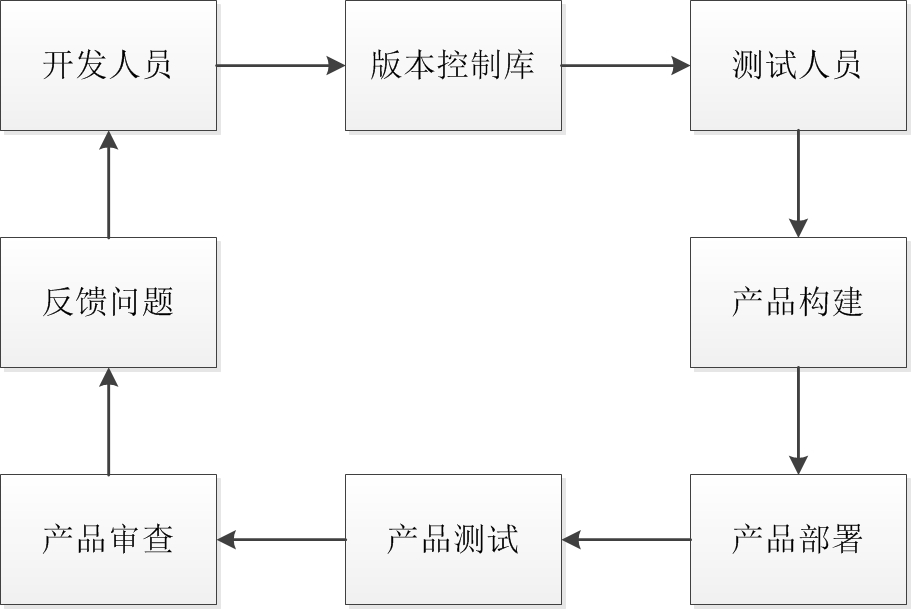
\includegraphics[height=7cm]{chart1/迭代式开发中的开发人员与测试人员的合作}
		\caption{迭代式开发过程中开发人员与测试人员之间的协作}
		\label{fig:迭代式开发中的开发人员与测试人员的合作}
	\end{figure}
  
\section{本文主要研究内容}

  \begin{itemize}
	\item 针对涉及到硬件的软件测试以及非OS下的软件测试,我们在基于EFI$\backslash$UEFI标准下,结合BIOS软件测试的实际需求,开发了一套测试工具SCT(Self-Certification Test:自我认证测试)~\cite{28, 29}用于对产品进行功能性测试,以验证产品中各种功能是否存在缺陷,对测试结果进行分析和总结以生成相应的报告。该测试工具在UEFI BIOS的Shell环境中~\cite{30, 31}运行,支持白盒、黑盒等不同类型的测试。总的来说,SCT具有以下几个特点:
	  \begin{itemize}
		\item 能够自动化的执行用例,对UEFI BIOS进行测试和验证,及时发现其中可能存在的问题和缺陷,以便于提高软件的质量。
		\item 能够执行多种测试类型,例如白盒、黑盒等不同类型测试。
		\item 能够分析每一个用例的执行结果,并且对全部用例的测试结果进行总结,生成相应的测试报告。
		\item 当工具运行发生意外中断时,能够记录中断的位置,在工具再次执行时从该位置继续执行之后的用例,而不需要对已执行的用例进行重复的测试。
		\item 具备良好的GUI,能够方便QA便捷的利用测试工具对测试用例进行管理和设置,控制需要执行的用例。
	  \end{itemize}
	\item 为了在有限的资源下,提高测试工作的效率、节省测试工作的成本、保证测试工作的进度和质量。我们搭建了一套可以无人值守的持续集成测试系统用于UEFI BIOS开发过程中每日的迭代性集成测试。该系统基于持续集成的思想,能够自动化的实现从产品构建、产品部署、利用SCT对其进行功能性测试、解析测试结果生成测试报告并且向开发人员反馈该系统测试出的产品缺陷这一系列复杂的测试流程,是持续集成理论的又一次成功实践。该系统总的来说具有以下几个特点:
	  \begin{itemize}
		\item 系统中的任一环节都是自动完成的,有利于减少测试任务中的重复过程所耗费的时间和人力成本。
		\item 系统能够尽早、及时的发现软件不能够构建或者存在产品缺陷的问题,使随时(快速、可靠、低风险)发布功能正常的软件成为了可能。
		\item 系统尽早、尽快进行集成,有助于尽早发现产品中存在的缺陷,避免最终产品集成中出现Bug(缺陷)大量涌现的情况,这样容易及时定位和修正Bug,提高产品开发的质量与效率。
		\item 保证了敏捷开发过程中软件项目的进度和质量。
	  \end{itemize}
  \end{itemize}

\section{论文的组织}
	
	第一章引言,介绍了课题的研究背景和现状,说明了选题依据和来源,简要的介绍了本文的工作,给出了本文的主要研究点和组织。
	
	第二章主要介绍了集成测试与持续集成测试的思想,针对现有CI引擎工具不满足UEFI BIOS的需求这一问题,提出了设计需求,为UEFI BIOS自动化测试系统的设计和实现做好了理论铺垫。
	
	第三章主要分析对比了现有的各种测试工具,针对其不适合非OS下的UEFI BIOS测试任务这一问题,设计并且实现了一款新的测试工具SCT专门用于UEFI BIOS的功能性测试,而产品测试的工作能够利用该工具在无人值守的情况下自动化的完成,正是持续集成测试系统中重要的组成部分。
	
	第四章主要介绍X-64架构(特定的CPU架构)的Denlow平台持续集成测试系统的设计与实现,并且展示了已经成功应用到Denlow-X64的实际开发项目中的系统实验结果。
	
	第五章主要介绍IA-32架构(特定的CPU架构)的Nt32平台持续集成测试系统的设计与实现,并且展示了已经成功应用到Nt32-IA32的实际开发项目中的系统实验结果。
	
	第六章对本文的工作的优缺点进行了归纳,并且提出了进一步的研究目标。
	
\section{本章小结}
  
    本章第一小节主要介绍了BIOS、UEFI、软件测试与UEFI BIOS软件测试的特点等这些课题的背景情况。
	
	本章第二小节主要介绍了测试工具和持续集成的研究情况。
	
	本章第三小节主要说明了本文的选题依据和来源,阐明了本文所具有的理论价值和实际应用价值。
	
	本章的第四小节说明了本文的主要研究内容。
	
	本章的第五小结说明了本文的组织情况。

	
\chapter{集成测试与持续集成测试}
\label{cha:intro}

本章首先对集成测试的理论和发展进行了概述,最后介绍了当前处于快速发展时期的敏捷开发所对应的持续集成测试,为后续UEFI BIOS自动化测试系统的设计与实现铺垫好了理论。

\section{集成测试}

\subsection{集成测试的概念}

  集成测试是一种旨在暴露模块单元接口之间、组件和系统间交互或者协同工作时所存在的缺陷的测试,重在接口的测试。它通过一定的方法,将已研发并且单独测试好的模块或者单元,通过设计好的产品规则集成为所需要的产品,并且测试该产品以保证产品能够正常的工作并且符合设计的目的,这一过程被称为集成测试。在进行集成时要注意下列几个注意点:
  
  \begin{itemize}
    \item 在将每个已经测试好的组成模块集成起来之后,经过模块输入输出接口的数据是不是会丢失。
	\item 某个正常执行的模块是不是会影响其他模块的正常工作。
	\item 每个各自正常工作功能的模块按照一定的需求和规则一起组合运行时,是不是能够完成设计所期待的效果。
	\item 全局的数据结构是否存在缺陷。
	\item 每一个模块可能都会存在误差,当他们积累到一起的时候,与期待结果的相差值会不会被放大,并且超过了设计时所不能接受的范围。
  \end{itemize}
  
  不同情况下不同层次的集成测试主要分为:

  \begin{itemize}
    \item 软件单元与软件单元的集成测试。
	\item 软件每个系统之间的集成测试。
	\item 软件系统和第三方系统的集成测试。
	\item 软件系统和硬件的集成测试。
  \end{itemize}
  
\subsection{软件开发模型与集成方法的对比研究}

  从集成方式看,瀑布模型对应的大棒集成、统一软件开发过程对应的渐增式集成以及敏捷软件开发中的持续集成,是最具有里程碑意义的三个阶段。如图~\ref{fig:从Big-Bang到持续集成的发展过程}所示:

  	\begin{figure}[H] % use float package if you want it here
		\centering
		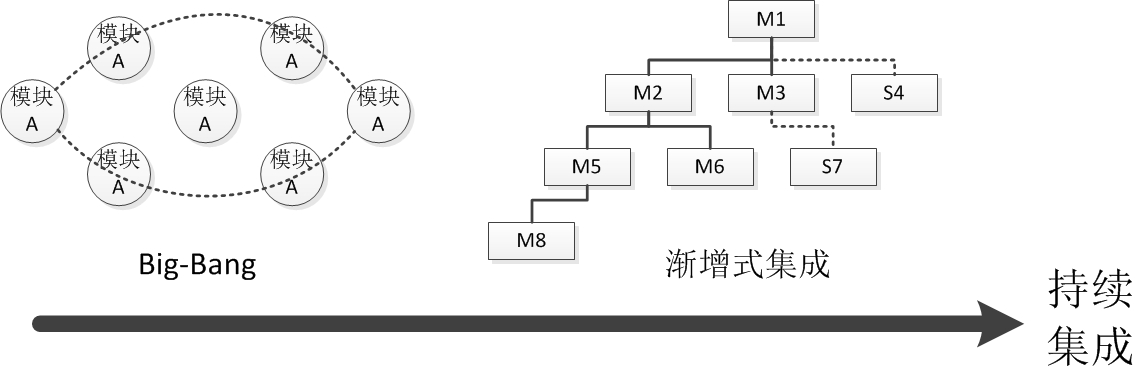
\includegraphics[height=4.8cm]{chart2/从Big-Bang到持续集成的发展过程}
		\caption{从Big-Bang到持续集成的发展过程}
		\label{fig:从Big-Bang到持续集成的发展过程}
	\end{figure}
  
  \begin{itemize}
	\item 瀑布模型与大棒集成模式
	
	Winston Royce~\cite{34}提出了瀑布模型~\cite{35},它认为软件产品研发的阶段应该分为五个,如图~\ref{fig:瀑布模型}所示:
	
	\begin{figure}[H] % use float package if you want it here
		\centering
		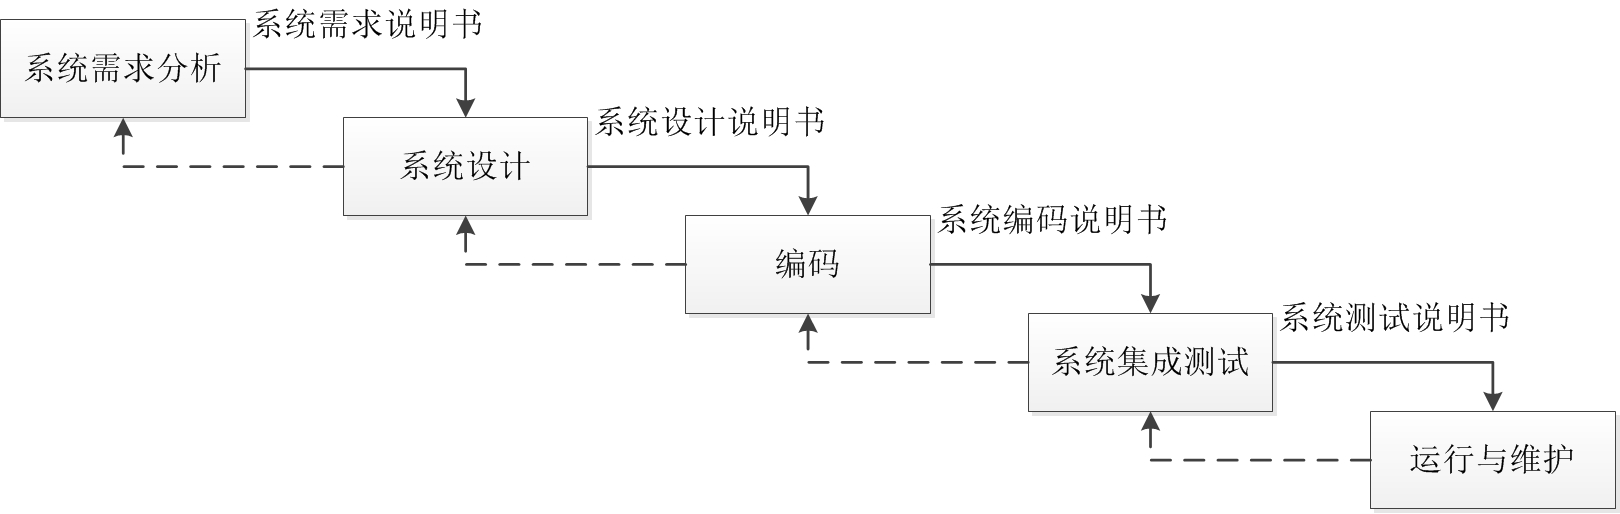
\includegraphics[height=4.5cm]{chart2/瀑布模型}
		\caption{瀑布模型}
		\label{fig:瀑布模型}
	\end{figure}
	
	当系统集成测试时各模块首次被结合起来之后,会有许多之前没有的问题涌现出来,其中一个模块出现问题之后,需要调试系统所有的部分才能定位缺陷的位置。通常把这种集成方式称之为大棒集成~\cite{36}。
	
	\item 统一软件开发过程与渐增式集成模式
			
	软件统一开发过程~\cite{37}认为,项目的开发应该通过数次迭代将其划分为若干个小的阶段,每一个迭代周期都应该包含各自对应的产品需求分析、系统设计、产品编码和软件测试等过程,每个周期结束后,应该对其结果按照各阶段的标准进行评判,若达到标准则制定下一周期的目标并且进入一轮新的迭代。如图~\ref{fig:迭代递增过程模型}所示:

	\begin{figure}[H] % use float package if you want it here
		\centering
		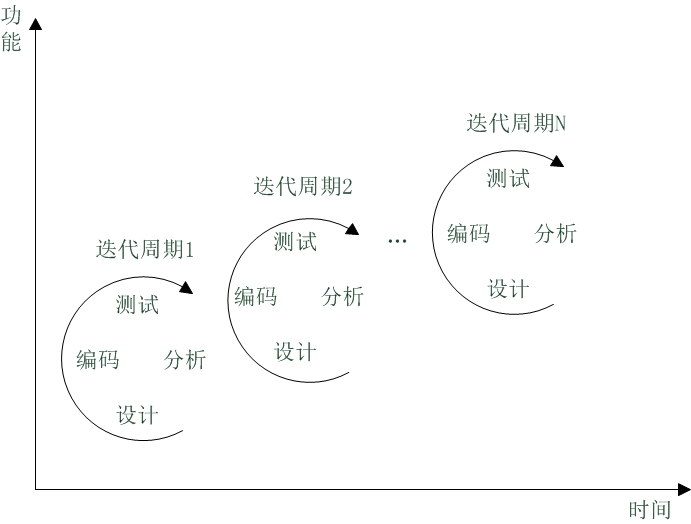
\includegraphics[height=7.5cm]{chart2/迭代递增过程模型}
		\caption{统一软件开发过程模型}
		\label{fig:迭代递增过程模型}
	\end{figure}
	
	\item 敏捷软件开发与持续集成
	
	敏捷开发方法~\cite{41}(Agile Methodologies,以下简称敏捷方法)针对现代商业软件业务复杂、需求频繁变化、开发周期短等问题,其通过以下几点来在整个软件开发的进程中大大缩减项目的成本:

	  \begin{itemize}
		\item 在产品开发开始后的第一到第三周尽快发布第一个版本,以便于能够尽快的得到反馈,并且在其基础上进一步开发。		
		\item 解决方案尽量不要太复杂,以便于在之后对其进行修改。
		\item 不断改进设计,提高设计的质量。
		\item 在每一个迭代的周期一直对产品测试和验证,从而在开发后期降低产品测试和缺陷改正的成本。
	  \end{itemize}
	
	敏捷软件开发方法认为,在对产品源文件做出一定修改后,就应当尽快集成和测试整个产品,反馈得到其结果,以验证之前的操作是否合理,这便是持续集成。
	
  \end{itemize}
  
  
\section{持续集成测试}

\subsection{持续集成的概念}

	作为持续集成的指导思想,软件开发者们认为,应该频繁的对整个软件产品项目的源代码库进行集成,甚至于任何一个对其的修改动作在提交到项目所对应的版本控制库之后,系统都应该触发一次针对该版本的集成工作,这对于整个软件项目工程的好处是非常大的,有助于产品缺陷及时暴露。而敏捷思想的重要体现之一,正是如何将软件的集成工作变为自动化的持续以及寻找最合适的极致点。~\cite{13}
	
	2006年,Martin Fowler阐述并且实现了持续集成这一重要思想:
	
	\begin{itemize}
		\item 软件产品项目的工程通常有大量的源文件,在产品的编译构建过程中需要包含数量庞大的文件,为了方便管理整个项目,应该创建单个产品的源码库,利用其保留所有这些文件的修改记录,并且这些修改记录是可以被追溯历史的,这一点非常重要。
		\item 在软件项目开发的过程中,开发者们会对产品的源代码进行频繁的重构和修改,在每次修改动作完成时,其都应该将本地修改的代码与源码库中的主干进行合并,频率上至少应该保证每天提交一次。这样有助于其他的软件开发人员清晰的了解源文件的变更情况,而少量的、及时的将修改提交到源码库,可以尽早的验证该操作的正确性,从而避免在产品后期集成时产品缺陷的集中涌现,大大减少代码回滚的成本以及修复产品缺陷的成本。
		\item 为了将产品的源码编译构建成为可正确执行的程序,软件开发人员通常需要从源码库中获取相应版本的产品源文件,并且利用相应的工具对产品的源码进行构建,将这些机械固定的操作利用相关的技术自动化的完成,有助于减少他们的时间成本,因此产品的构建过程需要能够自动化的完成。
		\item 为了保证开发人员对代码的每次修改操作的正确性,应该将其对应版本源码库中的源码进行集成构建。若构建失败则该操作错误,需要退回到修改之前的版本并且重新进行修改;若构建成功,则需要对产品进行环境部署并且加以相应的测试,已验证产品的正确性,如果存在产品的缺陷则应该及时的修复。
		\item 编译构建成功后的产品,应该部署到其相应的真实环境中去,并且利用相关的技术对产品进行测试,而这一系列的操作需要能够自动化的完成,而不需要人为机械的去手动操作。测试完成后,为了方便软件开发人员清晰的了解到最新版本产品的集成和测试结果,判断其对应的开发操作是否正确,持续集成系统应该能够自动的生成其对应的测试报告,并且将其按时反馈给每一个开发人员。
	\end{itemize}
	
	\begin{figure}[H] % use float package if you want it here
		\centering
		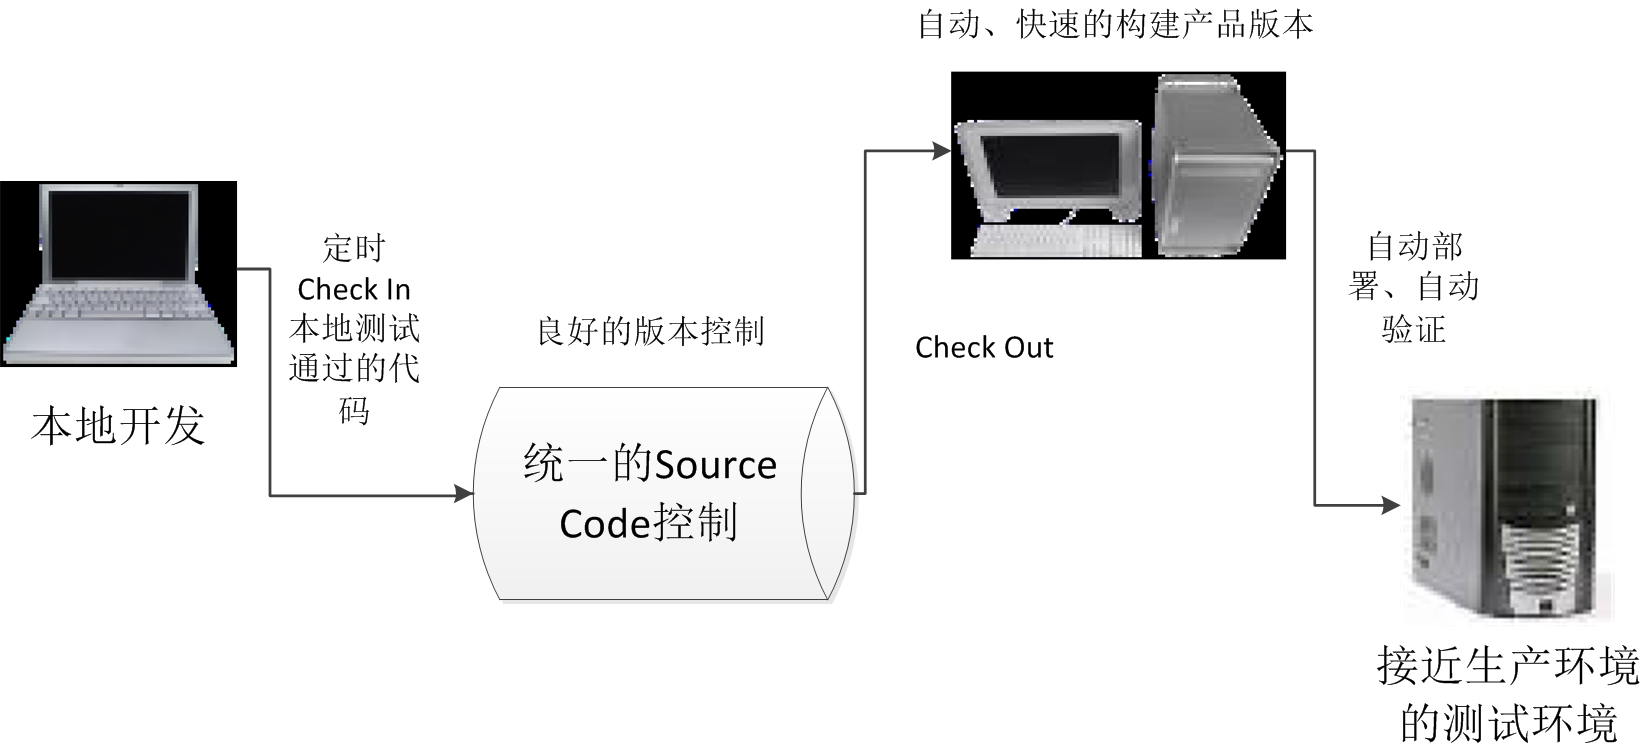
\includegraphics[height=6.5cm]{chart2/简化版持续集成}
		\caption{简化版持续集成}
		\label{fig:简化版持续集成}
	\end{figure}
	
\subsection{持续集成的价值}

	\begin{itemize}
		\item 系统中的任一环节都是自动完成的,有利于减少测试任务中的重复过程所耗费的时间和人力成本。
		\item 系统能够尽早、及时的发现软件不能够构建或者存在产品缺陷的问题,使随时(快速、可靠、低风险)发布功能正常的软件成为了可能。
		\item 系统尽早、尽快进行集成,有助于尽早发现产品中存在的缺陷,避免最终产品集成中出现Bug大量涌现的情况,这样容易及时定位和修正Bug,提高产品开发的质量与效率。
		\item 保证了敏捷开发过程中软件项目的进度和产品的质量。
	\end{itemize}
	
	\begin{figure}[H] % use float package if you want it here
		\centering
		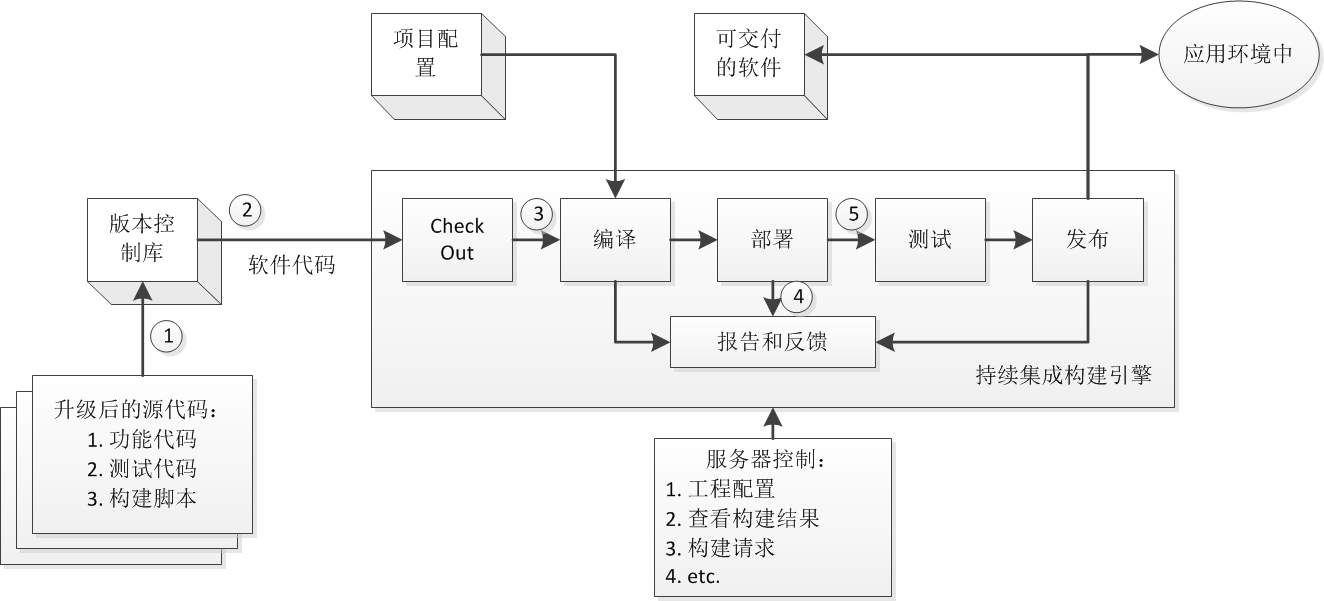
\includegraphics[height=7cm]{chart2/典型的持续集成开发场景}
		\caption{典型的持续集成开发场景}
		\label{fig:典型的持续集成开发场景}
	\end{figure}
	
\section{持续集成的组成}

	为了针对产品的特点,设计和开发的持续集成测试系统,其中所用到的每一个模块,以及其所组成的系统,都需要利用相应的自动化技术以及相应的工具。按照系统的需求,选择合适的技术与工具,寻求相应的方法与规则将它们结合到一起加以利用,才能够根据产品和测试操作的需求目的,实现其对应的系统,完成自动化的持续集成操作。这些工具和自动化技术如图~\ref{fig:与持续集成应用相关的软件工具和自动化技术}所示:
	
	\begin{figure}[H] % use float package if you want it here
		\centering
		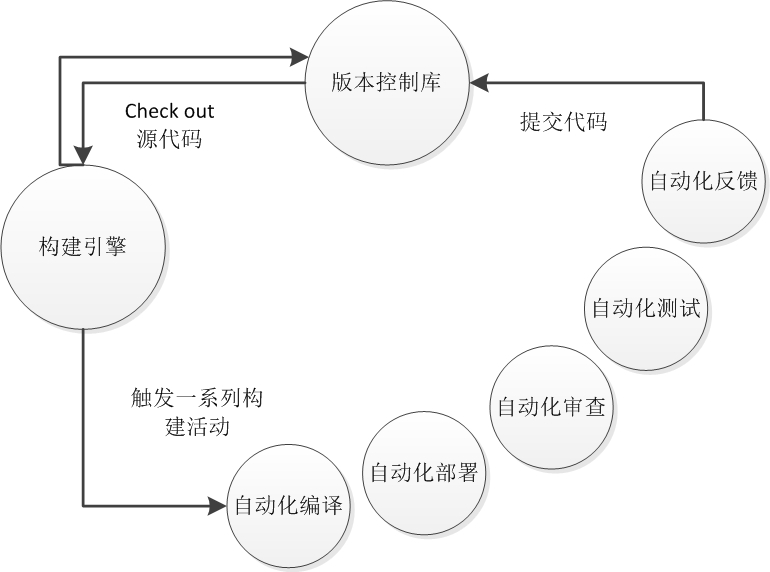
\includegraphics[height=7cm]{chart2/与持续集成应用相关的软件工具和自动化技术}
		\caption{与持续集成应用相关的软件工具和自动化技术}
		\label{fig:与持续集成应用相关的软件工具和自动化技术}
	\end{figure}
	
	这些自动化技术和相应的工具主要由产品的自动化构建技术、版本控制库、持续集成的构建引擎、版本控制系统所创建的版本控制库所组成。其中自动化构建与测试操作是CI持续集成测试系统的核心部分,由自动化编译构建、自动化产品测试、自动化审查、自动化环境部署、自动化报告反馈等技术组成。
	
	\subsection{持续集成的环境}
	
	持续集成的环境主要由图~\ref{fig:持续集成环境基本框架的体系结构图}中的各要素组成:
	
	\begin{figure}[H] % use float package if you want it here
		\centering
		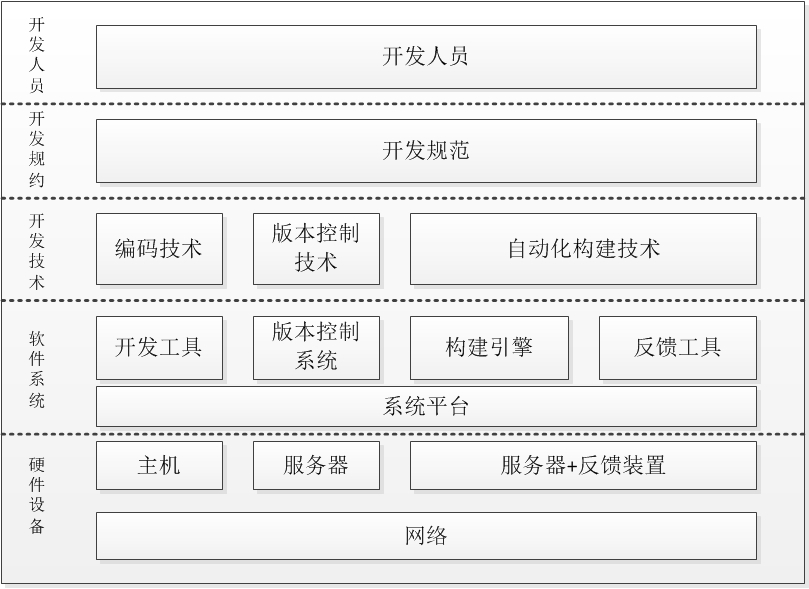
\includegraphics[height=8cm]{chart2/持续集成环境基本框架的体系结构图}
		\caption{CI环境基本框架的体系结构图}
		\label{fig:持续集成环境基本框架的体系结构图}
	\end{figure}
	
	\subsection{版本控制}

	软件产品工程的项目通常需要利用一个能够存放源代码的仓库来管理其对应的源文件,通常利用现有的版本控制系统来创建其对应的源代码仓库,利用其管理整个项目的源文件。版本控制系统能够进行有效的管理产品的源代码,开发人员在修改源码并对其提交后,版本控制系统都能够对其操作进行记录,并且在源码的修改出现问题时,利用其代码的可追溯性,根据代码的提交时间点,把源代码恢复到某个之前的版本。除此之外,利用其使得不同国家和地区的人们可以通过网络实现产品的协同开发。
	
	版本控制系统大致分为以下两种:
	
	\begin{itemize}
		\item 集中式版本控制系统
		
			集中式版本控制系统的原理,是利用一台服务器来保存所有修改版本的源文件,项目中共同协作的软件开发人员通过自己的客户端连接到这台服务器,服务器对其进行集中式的管理操作,开发人员可以利用各自的客户端从服务器中获取最新版本的源文件,并且能够将在本地修改的源文件作为新的版本提交更新到服务器中,为他人所获取。现如今常用的集中式版本控制系统主要有Subversion(SVN)、Concurrent Versions System(CVS)以及 Perforce 等。
			
			\begin{figure}[H] % use float package if you want it here
				\centering
				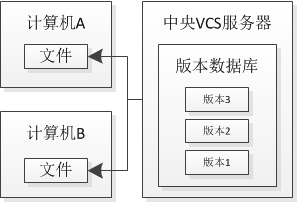
\includegraphics[height=5cm]{chart2/集中式版本控制系统}
				\caption{集中式版本控制系统}
				\label{fig:集中式版本控制系统}
			\end{figure}
		\item 分布式版本控制系统
		
			而在分布式版本控制系统中,每一个开发人员的计算机并不仅仅只是客户端,用于向版本控制库提交或者从版本控制库中提取最新一个版本的源文件,而且作为服务器把整个仓库全部作为镜像备份,每个成员可用于从中进行获取。开发人员对其的每一次克隆操作,事实上也都是完整备份所有版本的源代码仓库,所以当任何一处服务器发生故障无法正常运行时,其他的每一台服务器都有各自的一个镜像,并且可以利用对本地仓库来进行恢复。目前常用的集中式版本控制系统有Git、Mercurial、Bazaar 以及 Darcs 等,其中以Git最具有代表性和广泛使用性。
			
			\begin{figure}[H] % use float package if you want it here
				\centering
				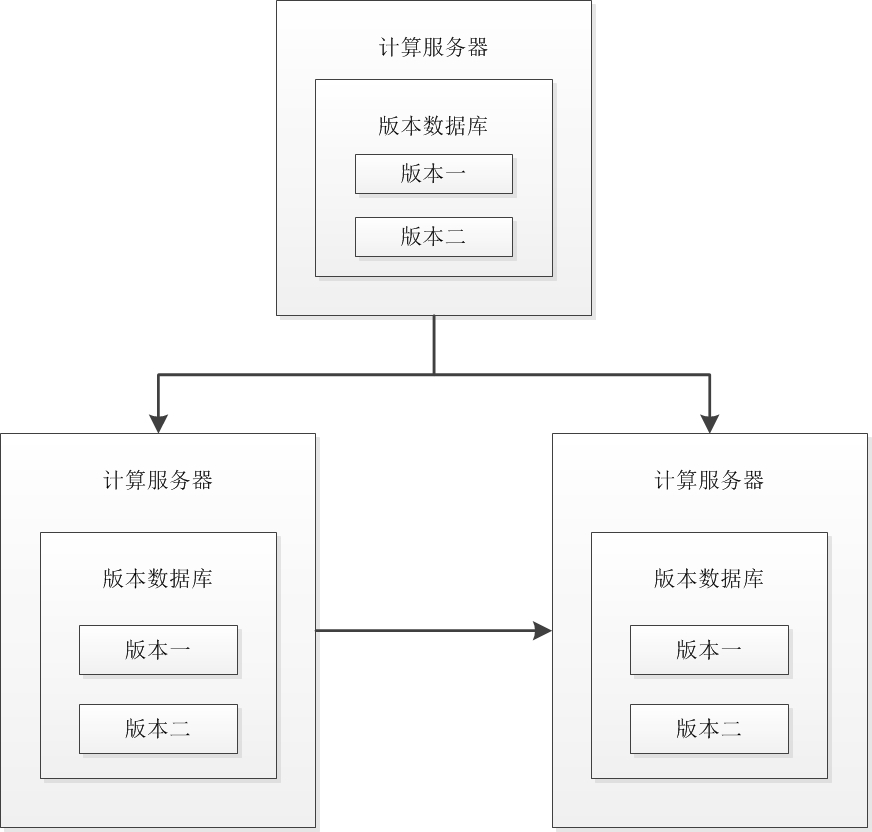
\includegraphics[height=9.5cm]{chart2/分布式版本控制系统}
				\caption{分布式版本控制系统}
				\label{fig:分布式版本控制系统}
			\end{figure}
	\end{itemize}

	\subsection{产品构建}
	
	产品构建环节,是指通过自动化编译技术将产品的源文件编译构建为可最终正常运行的可执行程序的过程。通常情况下利用现有成熟的自编译工具,即可完成产品的编译和构建,例如针对C、C++语言的Unix和Linux下的make工具、Java开发中的Jinx、Maven和Ant工具~\cite{43, 44, 45},以及.NET下的MSBuild工具。
	
	\subsection{环境部署}
	
	在产品构建完成之后系统对环境进行部署,执行如下流程:将已编译构建好的所需验证的可执行文件安装放置其相应的环境中,以便于后续对其进行相应的功能或者性能测试。实现自动化的环境部署的意义是令乏味、机械、重复的环境部署工作不需要人工去操作,从而大大节省了测试人员的成本。	
	
	\subsection{产品测试}
	
	产品测试是CI中最为关键的组成部分,用于检测出产品中存在的缺陷。CI的产品测试工作主要以单元测试~\cite{46}和功能测试为主,性能测试为辅。比较有代表性单元测试工具有:针对.NET 的nUnit、针对Python的pyUnit、针对C++的CppUnit、针对Delphi的dUnit等工具。利用这些现有的工具和技术,能够大大简化开发人员在不同平台和语言上的测试操作,节省他们的成本,提高测试的效率。
	
	\subsection{报告反馈}
	
	产品测试结束后,应该能够自动的解析测试结果生成测试报告,并且将产品的构建结果与测试结果以报告的形式通过电子邮件(Email)、Socket、FTP、HTTP、聚合内容(RSS)等形式途径,及时快速的反馈到所有项目相关的软件开发与测试人员手中,这就是测试反馈部分所需要做的工作内容。
	
\section{现有的持续集成引擎的分析与对比}
	
	为了实现持续集成的自动化,需要使用合适的技术和途径,及时发现版本控制库中源文件的修改与变更情况,若出现变更,应及时自动化的触发集成测试任务,自动化的完成从产品构建、环境部署以及产品测试的过程,并且利用自动化测试反馈的技术,解析测试结果自动生成相应的测试报告,并通过2.3.6小结所提到的形式及时迅速的将结果反馈给开发人员。而这一过程的控制主要由持续集成引擎完成,它是使集成测试做到持续的关键所在。
	
	\subsection{现有的持续集成引擎}
	
	目前专用于持续集成的引擎越来越多,其中常用到的产品有:Cruisecontrol~\cite{47}、Jenkins、QuickBuild和Anthill~\cite{48}等。以下简单介绍两款常用的产品:

	\begin{itemize}
		\item CruiseControl
		
		CruiseControl是最早出现的持续集成引擎之一,由Build Loop作为主体和部分插件所构成。其主体使用轮询机制来定时检测产品源代码的版本,当发现版本更改之后,其可以读取config.xml配置文件中的配置信息,利用其作为准则,调用例如:Ant、Maven等相应的构建工具,以对产品进行自动化的构建。利用RSS、IM、Email 等反馈策略,CruiseControl能够将产品构建的结果尽早、及时的反馈给项目组中相关的成员,以保证最新版本的源代码的有效性。
		\item Jenkins
		
		作为开源软件的代表作之一,Jenkins这款持续集成引擎工具,近些年来在市场中的占有率在不断提升,其广泛应用的程度可想而知。Jenkins具备支持插件、简单的配置安装、监控的可视化这一些特点功能,不仅如此,其具有较快的版本更新能力,通常会每周一次进行版本更新,此外不得不提的是其在GitHub上具备较强的主导能力。这一系列的特点使得这款工具成为了持续集成引擎的代表作,并且在持续集成这一领域的占有率遥遥领先。~\cite{26, 27}
	\end{itemize}
	
	\subsection{现有持续集成引擎的对比}
	
	现有几款常用的持续集成引擎的对比如表~\ref{tab:现有几款主流持续集成引擎的对比}所示:
	
	\begin{table}[H]
		\centering
		\caption{现有几款主流持续集成引擎的对比}
		\label{tab:现有几款主流持续集成引擎的对比}
		\begin{center}
		\begin{tabular}{|p{2.4cm}|p{3.8cm}|p{3.8cm}|p{3.8cm}|} 
		\hline
		{\diagbox[width=2.8cm]{属性}{种类}} & Jenkins & QuickBuild & CruiseControl \\ \hline
		运行的操作系统环境 & 所有的操作系统平台 & Windows 、Linux、Solaris等操作系统平台 & Windows、Unix、Linux以及任何能够正常运行Java虚拟机的操作系统平台 \\ \hline
		特点 & 目前应用最广的集成服务器,具备强大的可扩展插件的特点,开源 & 大型公司对其较多使用,可跨多种平台 & 较适合.NET 开发与Java开发,可跨平台使用 \\ \hline
		可扩展性 & 具备较强的可扩展性,插件库中的内容丰富,可选择程度较高 & 商业软件,不可扩展 & 可扩展,有较多现有的插件供使用 \\ \hline
		版本控制系统的可支持性 & 支持Subversion、CVS、ClearCase、Git等所有主流的集中式与非集中式版本控制系统 & 常用的版本控制系统均可支持使用,较新的版本对GitHub进行了集成 & Subversion、CVS、ClearCase等集中式版本控制系统 \\ \hline
		更新频率 & 更新频率极高 & 更新频率较高 & 版本较旧,更新频率较低 \\ \hline
		易用性 & 极为易用,便于快速部署搭建,维护起来较为简单,具备多种启动方式 & 较为易用,且可用其对大集群服务器进行部署,稳定 & 较难使用,部署和维护的成本高,配置文件过多不利于使用 \\ \hline
		\end{tabular}
		\end{center}
	\end{table}
	
\section{现有持续集成与UEFI BIOS持续集成的分析与对比}
	
	UEFI BIOS产品的开发是一个长期的项目,项目的开发采用敏捷开发的方式,在开发过程中,每一个短暂的迭代周期都会对代码进行频繁的重构和修改,每一次修改都会产生一个新版本的可执行产品,因此QA需要尽早对产品进行集成和测试,这样可以大大避免在项目后期产品进行集成时出现产品缺陷集中涌现的问题。然而随着项目开发过程的进行,QA的测试工作任务量会不断的提升和累加,如果采用手动测试机械重复的完成这些繁重的测试任务,毫无疑问是不明智也是低效的,因此为了节省测试工作的时间和人力成本、提高测试工作的执行效率、保障测试工作的顺利进行和高质量进行,搭建一个自动化持续集成测试系统用于完成从产品构建、产品部署、产品测试以及产品质量分析的UEFI BIOS集成测试工作就显得非常必要。
	
	由于现有的持续集成的各个阶段均是工作在OS(Operation System,操作系统)中的,而UEFI BIOS是工作在OS(Operation System)之下,其源代码的管理、产品的构建虽然是在OS中完成的,但是其环境的部署、产品的测试需要涉及到在非OS的情况下完成,因此现有的各种CI引擎、环境部署和自动化测试工具并不能够实际的应用到UEFI BIOS的测试工作中,需要寻求新的解决方法,甚至开发新的工具,并且利用合适的技术将持续集成的各个阶段在OS与非OS的情况整合到一起,来完成该套UEFI BIOS持续集成测试系统的开发。
	
	针对不同CPU架构以及不同的计算机硬件环境,UEFI BIOS的分类有很多种。在本论文中,我们以Denlow和Nt32两种平台为例,来说明在这两种平台下的自动化测试系统框架的搭建。最终的完成目标是:在IA-32架构(特定的CPU架构)的Nt32平台和X-64架构(特定的CPU架构)的Denlow平台上,实现对该两种不同架构的不同平台的UEFI BIOS持续集成测试系统的搭建。
	
\section{本章小结}
    本章首先对集成测试理论的发展进行了概述,最后介绍了当前处于快速发展时期的敏捷开发所对应的持续集成测试,为后续UEFI BIOS自动化持续集成测试系统的搭建奠定了理论基础。
	
	2.5小结主要将现有持续集成技术与UEFI BIOS持续集成的需求进行了对比。
\chapter{UEFI BIOS自动化测试工具SCT的设计与实现}
\label{cha:intro}
	
	UEFI BIOS作为新一代的BIOS,在其开发过程中,需要开发人员对源文件频繁地进行重构,这就需要对其的测试工作是可以自动化、简洁、高速运行的,否则代码的重构也就是不现实的。与传统的软件测试工作相比而言,UEFI BIOS的软件测试工作与之有着很多的不同点:UEFI BIOS软件的运行并不是在OS(Operating System:操作系统)环境中,而是在计算机加载操作系统之前运行,而现有的测试工具均是运行在操作系统环境之中的,因而现有的测试工具均无法正常运行在UEFI BIOS环境中,在被测机器上对其进行测试。而利用测试工具对已构建、部署好的产品进行验证和测试同样也是UEFI BIOS持续集成测试系统的基础。 因此,设计一套拥有良好性能和稳定可靠的测试工具用于UEFI BIOS的测试就成为了我们首先要解决的问题。
	
\section{自动化测试工具的设计目标}

	在基于EFI$\backslash$UEFI标准下,我们需要结合UEFI BIOS中测试的实际需求,开发一套自动化测试工具SCT用于测试UEFI BIOS中各种类库的正确性和有效性。SCT能够在UEFI BIOS的Shell环境中运行,对产品进行白盒、黑盒等不同类型的测试,自动化的执行用例以对产品进行验证,并且能够以测试报告的形式作为结果,便于QA对测试整体进行查看。
	
\section{ 自动化测试工具的需求分析}

  该测试工具需要具有以下特点:

  \begin{itemize}
    \item 能够自动化的执行用例,对UEFI BIOS进行测试和验证,及时发现其中可能存在的问题和缺陷,以便于提高软件的质量。
	\item 需要能够执行多种类型的测试任务,例如白盒、黑盒等不同类型的测试。
	\item 能够分析每一个用例的测试结果和日志,对全部用例进行总结,生成相应的测试报告。
	\item 具备完善的日志功能,便于QA查看测试工具的运行记录。
	\item 当工具运行发生意外中断时,能够记录中断的位置,在工具再次执行时从该位置继续执行之后的用例。
	\item 需要具备良好的GUI,方便QA能够便捷的对测试工具进行设置,控制需要执行的用例。
	\item 由于良好的扩展性是产品的一个特点,因此工具应该具备方便添加相应的测试库这一重要的功能属性。
  \end{itemize}

\section{自动化测试工具的系统功能组成分析}

	根据对SCT的需求进行分析和归纳,本文进一步对其系统的各个组成功能进行了设计,得出最终的UEFI BIOS测试工具SCT的系统功能组成框架如图~\ref{fig:自动化测试工具的功能组成框架图}所示:
	
	\begin{figure}[H] % use float package if you want it here
		\centering
		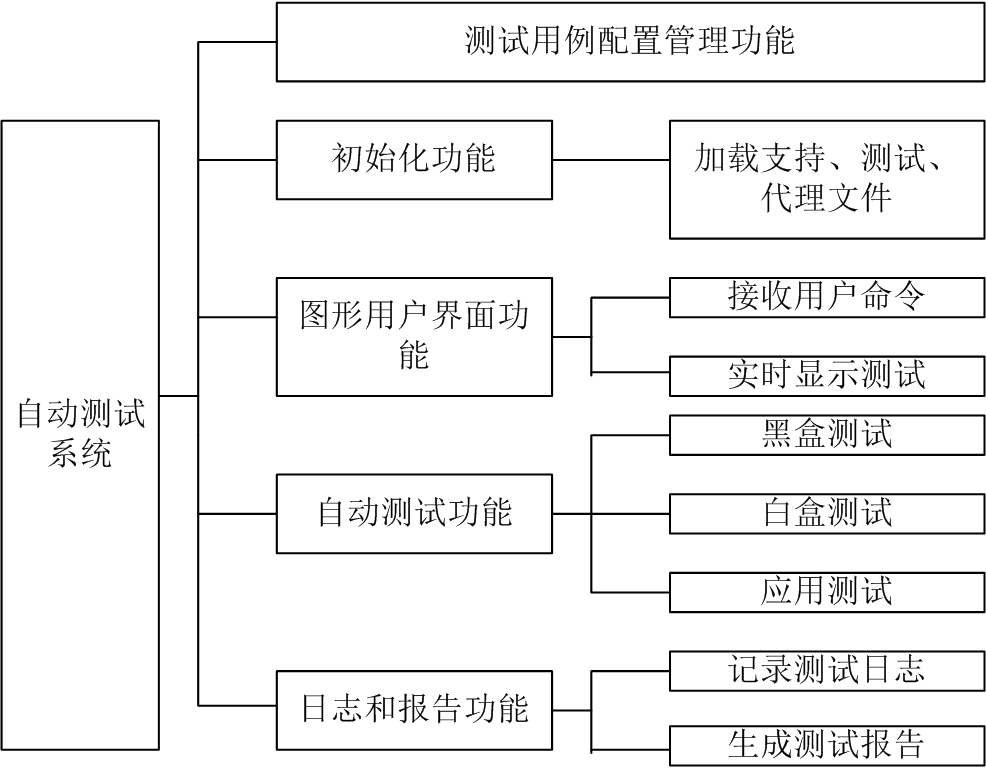
\includegraphics[height=8cm]{chart3/自动化测试工具的功能组成框架图}
		\caption{自动化测试工具的功能组成框架图}
		\label{fig:自动化测试工具的功能组成框架图}
	\end{figure}
	
	\begin{itemize}
		\item 用例配置管理的功能
		
		SCT需要在运行并对产品进行测试之前首先进行配置,主要是通过加载配置文件的方法来实现该功能。将对一切用例文件的描述信息存入到一个配置文件里,测试工具启动运行时对其进行读取并且使用。
		\item 初始化的功能
		
		在工具启动时自动加载测试、代理和支持文件,而这些文件也正是工具所必须的文件,这一功能即为初始化功能。所加载的各种文件是提前通过编译构建好的可执行文件,这些文件的后缀为.efi。测试工具SCT在运行测试任务时,每一个测试文件都有相对应的代理文件与之匹配,通过代理文件其读取所需要测试功能函数的相关信息,以便于验证该函数的正确性。
		\item 图形用户界面的功能
		
		GUI用于展示工具中的用例及策略,按照QA的思路便于QA对策略进行修改,并且能够实时的将测试的相关信息在测试前、中、后展示给QA,在测试后将每一个Case的执行情况以及执行结果通过GUI展示给相关的QA。
		\item 自动化测试的功能
		
		SCT的核心功能部分便是自动化测试功能,它按照QA的意愿对其所需执行的用例自动化的执行。工具运行对测试文件进行加载,操纵测试的进度,自动化的寻找并且执行下一个用例。当出现中断问题时,工具会对此次的中断点进行储存,工具再次运行时会首先提示QA是否在断点的基础上执行之后未完成的部分,这大大提高了测试的可持续性。
		\item 日志和生成报告的功能
		
		SCT能够将对每个Case的执行情况和结果进行记录,并且根据这些记录QA能够利用SCT自动化的生成该轮测试任务的报告,这就是日志和生成报告的功能。这一功能便于QA从整体上来观察和判断此轮测试任务的进展和结果。SCT将每一个Case的运行情况和结果自动记录到其对应的每一个日志文件当中,利用这一些日志文件,SCT能够自动化的生成CSV报告,它能够对所有的用例的执行结果进行概括。
	\end{itemize}
	
\section{自动化测试工具的系统功能流程分析}
	
	QA首先将用例和代理文件放在测试工具相应的目录下,SCT运行时首先进行初始化,通过配置文件的管理加载所需要的用例,将所需要的文件载入到测试工具中,并且提取出文件中包含的测试单元和用例,进入图形化用户操作界面。之后QA通过GUI选择、配置、执行用例,SCT就自动化的运行已选的用例,进行白盒、黑盒测试,同时生成相关的日志。任务完成后QA通过SCT提供的功能能够自动化的生成初步的报告。
	
	综上所述,可以得出UEFI BIOS测试工具SCT的系统功能流程如图~\ref{fig:自动化测试工具的功能流程图}所示:
	
	\begin{figure}[H] % use float package if you want it here
		\centering
		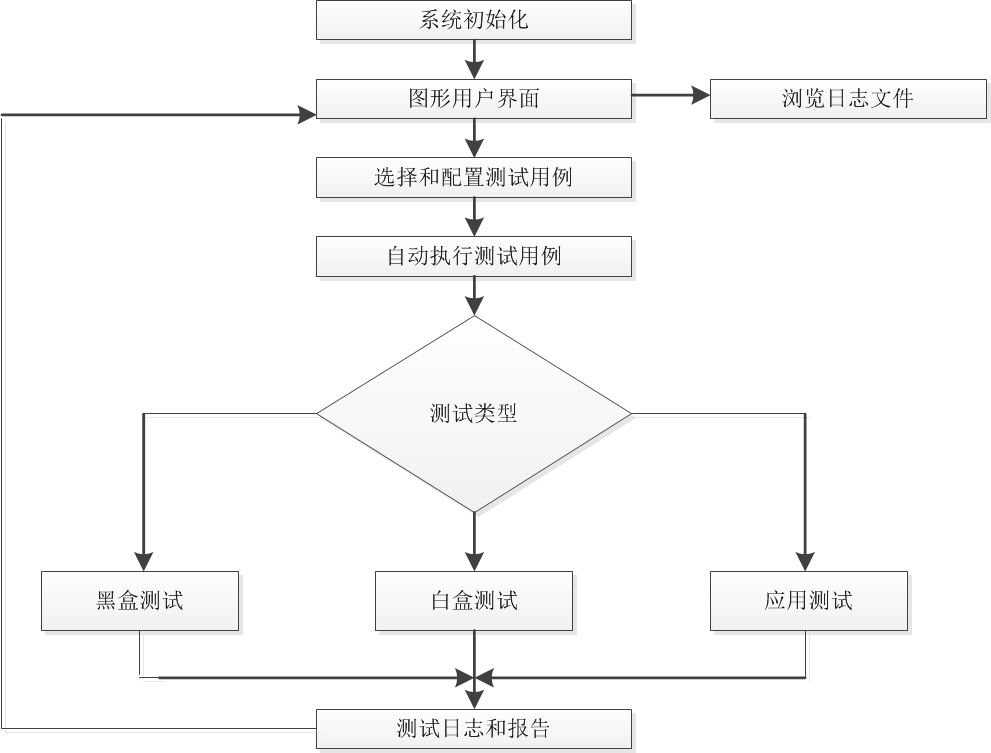
\includegraphics[height=10cm]{chart3/自动化测试工具的功能流程图}
		\caption{自动化测试工具的功能流程图}
		\label{fig:自动化测试工具的功能流程图}
	\end{figure}
	
\section{自动化测试工具的设计方案}
	
	在分析了测试工具的功能组成架构和功能流程的基础上,本小节将对该系统主要功能的设计和实现进行描述。
	
	\subsection{自动化测试工具中储存结构的设计及文件的载入}
		
		SCT储存的结构分为外部和内部两部分,外部的储存由配置文件和日志文件两部分组成,内部的储存则是文件以及Case在SCT内部结构的描述,这一小节我们主要对其进行讨论。
		
		\begin{itemize}
			\item 测试函数库以及测试用例管理配置的详细设计
				\begin{itemize}
					\item 测试库配置管理
					
					在工具启动并初始化以及在用例执行时,我们需要寻找合适的方法向用户提供一些被测试函数库的描述信息供其使用。考虑到被测试函数库的信息在项目开发的进行中是基本不会被修改的,因此我们创建一个文件夹,利用配置文件来存储所有的被测试函数库的基本信息,供测试工具加载使用。
						
					针对配置文件中的信息格式,我们设计了五个属性用于对被测试函数库进行描述,主要由Revision、CategoryGuid、InterfaceGuid、Name和Description构成。其中Revision代表被测试函数库的产品版本号,所有被测试函数库的版本号通常情况下都是0x00010000;CategoryGuid代表该被测试函数库的唯一标识;InterfaceGuid代表该被测试函数库的一个实例的GUID,其中GUID是UEFI BIOS开发中针对每个函数库以及其实例所设定的一个唯一的标识;Name代表被测试函数库的名称;Description代表被测试函数库的描述信息。以GenericTest为例它的配置信息如图~\ref{fig:测试库配置管理中配置信息的设计}所示:
						\begin{figure}[H] % use float package if you want it here
							\centering
							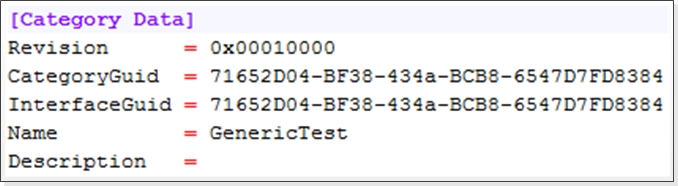
\includegraphics[height=3cm]{chart3/测试库配置管理中配置信息的设计}
							\caption{测试库配置管理中配置信息的设计}
							\label{fig:测试库配置管理中配置信息的设计}
						\end{figure}
							
					.ini文件为UEFI BIOS所规定的配置文件格式,所以设计的配置文件,其命名为Category.ini,其中包含了所有被测试函数库的相关信息,SCT在启动运行时自动加载该配置文件并且读取其中的内容,从而获取所有被测试函数的描述信息。
					
					\item 用例配置管理
					
						一个测试用例对应一个被测试函数,被测试函数库由相应的测试用例集所对应,为了存储测试用例的相关描述内容,我们创建了一个文件用于保存这些内容,这个文件叫做Seq.seq,用以在自动化测试工具中保存测试用例的信息。每一个测试用例的信息由四部分内容所组成:Revision代表测试用例的版本号,通常情况下其默认版本号为0x10000;GUID代表UEFI BIOS规定的被测试函数的唯一标识;Name代表被测试的函数,即被测试函数的名称;Order代表此用例在该轮测试的执行顺序,通常其默认值为0xFFFFFFFF,自动化测试工具会按照该配置文件中测试用例的顺序依次执行;Iterations代表该测试用例被迭代测试的次数。以GetState-Func函数为例,其对应测试用例的配置信息如图~\ref{fig:测试用例配置管理中配置信息的设计}所示:
							\begin{figure}[H] % use float package if you want it here
								\centering
								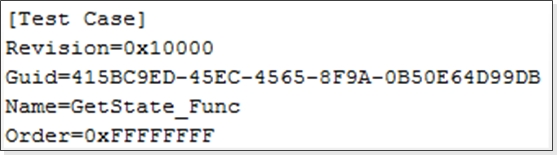
\includegraphics[height=3cm]{chart3/测试用例配置管理中配置信息的设计}
								\caption{测试用例配置管理中配置信息的设计}
								\label{fig:测试用例配置管理中配置信息的设计}
							\end{figure}
				\end{itemize}
			\item 文件结构和用例结构详细设计
			
				SCT自动化测试工具需要在启动并且运行时加载四类文件,其中包括配置文件、代理文件、支持文件以及测试文件。为了载入这四类文件,SCT在启动运行后,加载并且遍历该四类文件各自所属文件夹下的所有内容,其以整个文件目录为目标进行加载,在加载后对其进行判断,若是所需文件,则以文件为单元,载入到计算机内存中便于后续对其使用。为了支持系统例如恢复、日志和Assertion等功能,本文将这些功能通过.efi文件的形式进行实现,并且以主目录下Support文件夹的Driver文件以及Application文件等形式进行存放,SCT启动运行后便会加载这些.efi文件从而实现这一系列的功能。为了将载入工具中的剩余文件在系统中保存,我们利用结构体和链表的形式对其进行设计和实现,来保存其他的文件。
		\end{itemize}
	\subsection{自动化测试工具的各个模块设计}
		
		整个SCT由四部分功能模块共同构成:GUI图形用户操作界面、自动化测试运行、SCT初始化、日志和报告反馈这四部分模块。若干个小的功能模块构成了每一个模块部分,其整体结构组成如图~\ref{fig:自动化测试工具的纵向结构图}所示。下面是有关各个模块详细设计的讨论。
		
		\begin{figure}[H] % use float package if you want it here
			\centering
			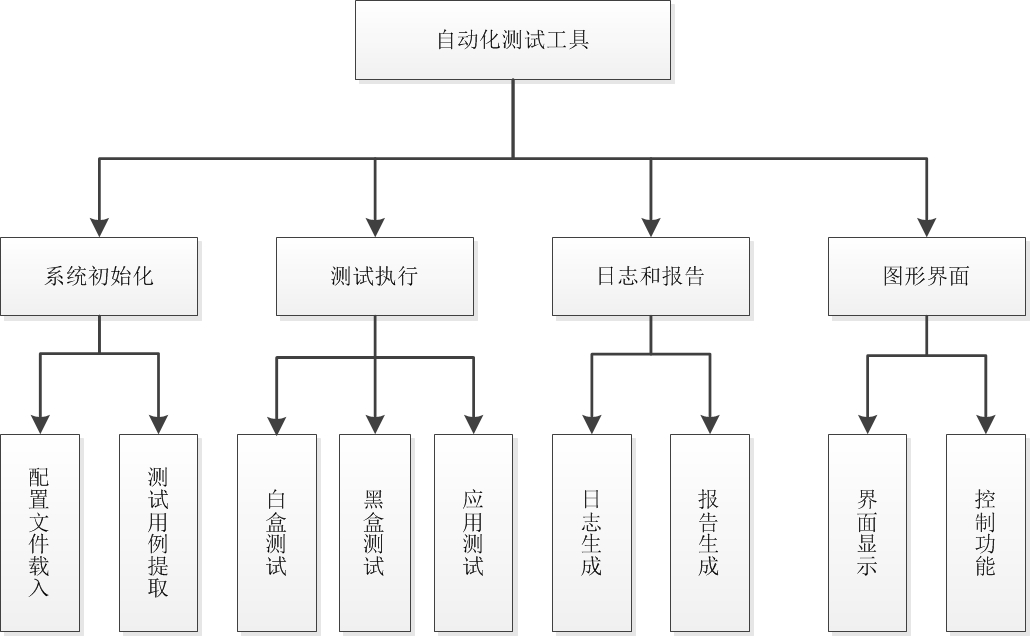
\includegraphics[height=8cm]{chart3/自动化测试工具的纵向结构图}
			\caption{自动化测试工具的纵向结构图}
			\label{fig:自动化测试工具的纵向结构图}
		\end{figure}
		
		\begin{itemize}
			\item 初始化模块详细设计
			
				该模块是对SCT启动并且初始化进行支持,它将SCT所需的文件加载,读取所有用例和初始化用例的状态。其主要分为两个部分:第一个部分为SCT载入代理、配置文件;第二个部分为SCT加载测试文件,并且从中提取Case的相关内容,从而确定该轮测试任务所要执行用例的情况,并且设定测试用例的状态。其流程如图~\ref{fig:初始化模块流程图}所示:
			
				\begin{figure}[H] % use float package if you want it here
					\centering
					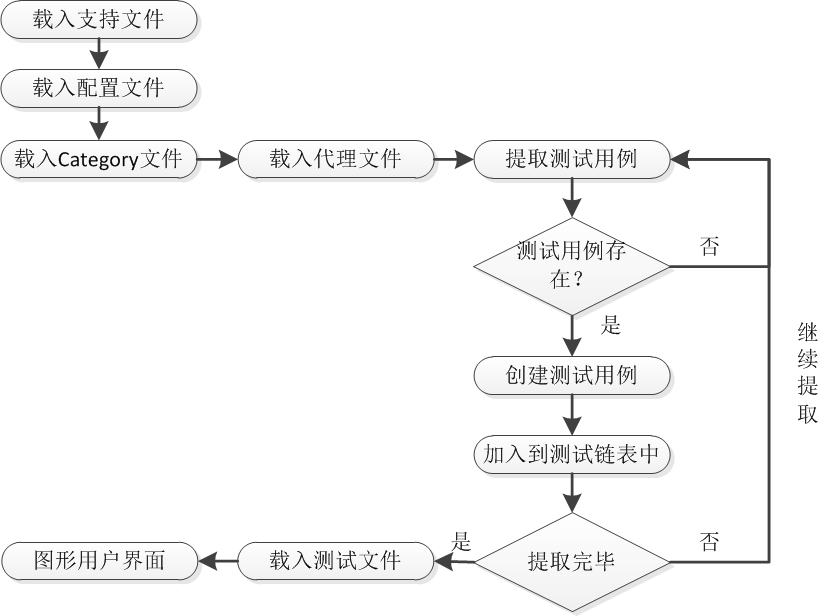
\includegraphics[height=9cm]{chart3/初始化模块流程图}
					\caption{初始化模块流程图}
					\label{fig:初始化模块流程图}
				\end{figure}
			
			\item 自动化执行模块详细设计
			
				有两种方法可以用于自动化的运行测试:第一种是通过GUI,QA利用键盘等外设选择该轮测试任务所需要执行的Case,然后选择执行,SCT便会对其自动化的执行各种类型的测试任务;第二种则是QA通过在SCT运行前修改和设置文件配置相关信息,从而通过其文件中指定的执行所需用例,这样能够通过配置文件提前将每轮测试任务所需要执行的Case提前设置好,而不需要每次通过第一种方法GUI界面操作的方法来对其进行设置。自动化执行模块的功能流程如图~\ref{fig:自动化执行模块流程图}、~\ref{fig:自动化执行模块中测试功能部分的流程设计}所示:
			
				\begin{figure}[H] % use float package if you want it here
					\centering
					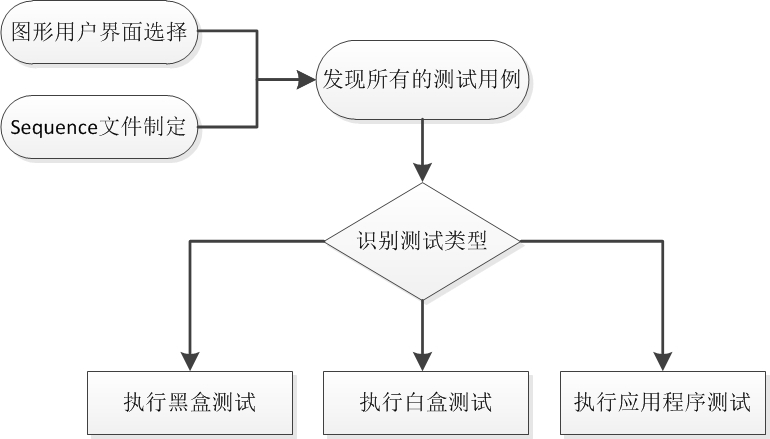
\includegraphics[height=6.5cm]{chart3/自动化执行模块流程图}
					\caption{自动化执行模块流程图}
					\label{fig:自动化执行模块流程图}
				\end{figure}
			
				\begin{figure}[H] % use float package if you want it here
					\centering
					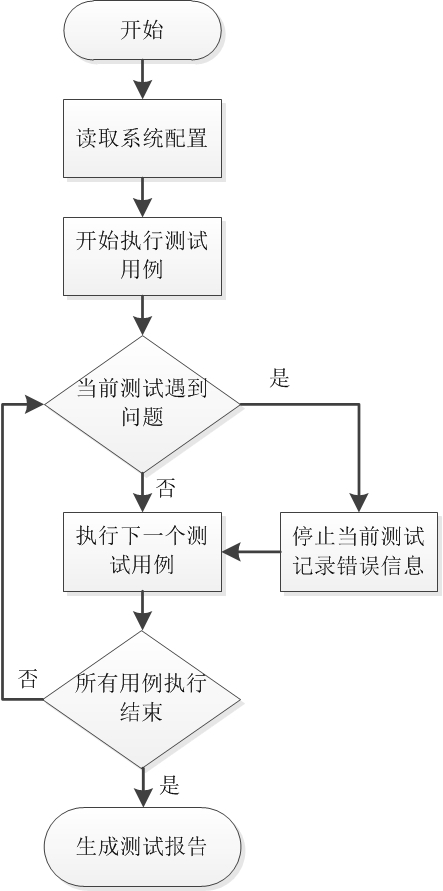
\includegraphics[height=14cm]{chart3/自动化执行模块中测试功能部分的流程设计}
					\caption{自动化执行模块中测试功能部分的流程设计}
					\label{fig:自动化执行模块中测试功能部分的流程设计}
				\end{figure}		
			
			\item 日志和报告模块详细设计
				\begin{itemize}
					\item 日志部分设计
					
						每一运行的用例由一个日志文件相对应,文件中的信息分为7个部分,如图~\ref{fig:日志文件设计图}所示:
						
						\begin{figure}[H] % use float package if you want it here
							\centering
							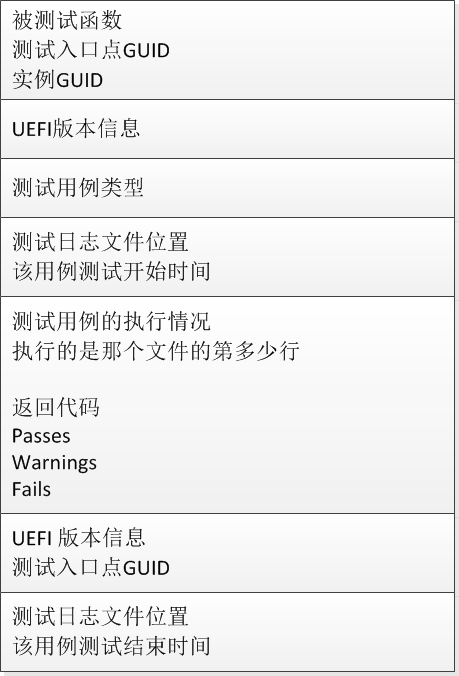
\includegraphics[height=11cm]{chart3/日志文件设计图}
							\caption{日志文件设计图}
							\label{fig:日志文件设计图}
						\end{figure}
						
						为了实现测试日志这一功能,SCT利用支持文件对其进行设计与实现。为了向SCT提供需要测试的功能,本文将测试日志部分设计成为驱动,在SCT启动并且初始化时,首先将该驱动加载到工具中。和面向对象设计中的类相似,本文将自动化测试工具中实现测试功能的部分设计为Protocol,由数据成员和相应的功能函数所构成,其名称为TLL(Test Logging Library)。TLL由构造函数TLLBeginLogging、析构函数TLLEndLogging和其他一些功能函数共同组成。TLLBeginLogging的主要功能为:加载所需被运行测试用例的相关内容,为测试日志的生成在操作系统中提前分配好所需的空间内存,创建好所需的相关结构体,并且打开日志文件对其测试执行过程中的相关信息进行记录。TLLEndLogging的主要功能为:关闭打开的日志文件,释放之前分配的内存空间。我们还设计了一个函数命名为TLLSetConfig,用于在自动化测试工具启动时对其日志模块进行设置。在设计好的日志功能中,还有一个最为重要的函数TLLWriteLogFile,他的主要功能是将测试过程中的日志信息写入到相关的日志文件中。综上所述,日志功能的设计如图~\ref{fig:日志功能的设计表}所示:
						
						\begin{figure}[H] % use float package if you want it here
							\centering
							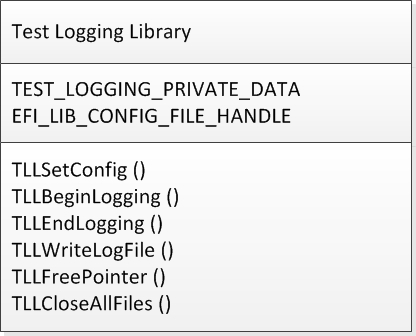
\includegraphics[height=6cm]{chart3/日志功能的设计表}
							\caption{日志功能的设计表}
							\label{fig:日志功能的设计表}
						\end{figure}	
					
					\item 报告部分设计
					
						该模块是SCT的一个重要组成功能,它以日志为基础,对此次测试验证的结果进行统计和概述,其内容主要包含用例的数量,每个用例的执行结果等相关信息,这使得QA节省了自己动手统计的时间成本。
						
						针对报告中信息的格式的设计,以测试需求为基础,将其分为两部分内容:第一部分为概述信息,说明了所测试函数的名称、用例的总个数、失败用例以及通过用例的数量;第二部分则是测试过程中的相关信息,未通过在前通过的在后。如图~\ref{fig:测试报告文件格式设计}所示:
						
						\begin{figure}[H] % use float package if you want it here
							\centering
							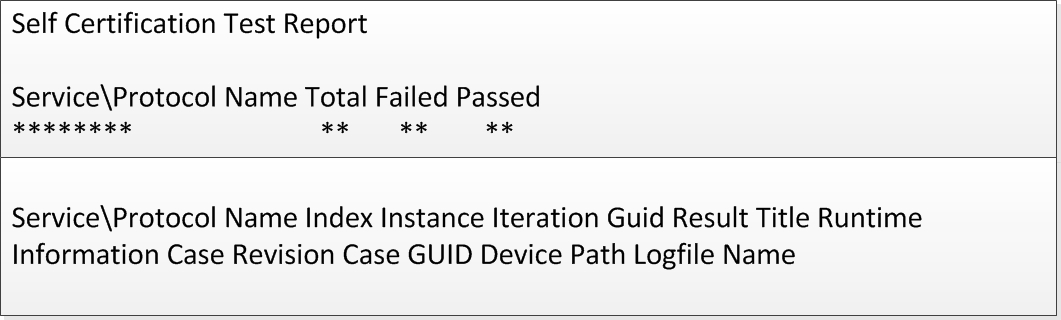
\includegraphics[height=3.7cm]{chart3/测试报告文件格式设计}
							\caption{测试报告文件格式设计}
							\label{fig:测试报告文件格式设计}
						\end{figure}	
						
						该格式的报告,不仅对本轮测试进行了概述,同时也对每一个用例进行了详细的描述,这便于QA能够对本轮测试工作每一个Case的进展进行清楚地了解。
					\item 测试报告生成流程设计
					
						测试报告的自动生成,是指SCT通过测试过程中产生的日志文件,对其中的信息进行解析和总结,从而形成测试报告文件,便于QA从整体上来把握此轮测试的结果这一重要的过程。本文设计好的该过程的流程如图~\ref{fig:测试报告生成流程图}所示:
						
						\begin{figure}[H] % use float package if you want it here
							\centering
							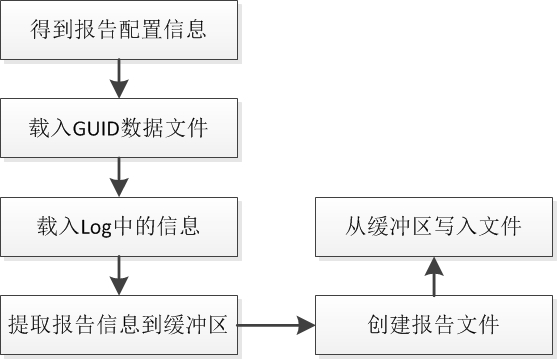
\includegraphics[height=6.5cm]{chart3/测试报告生成流程图}
							\caption{测试报告生成流程图}
							\label{fig:测试报告生成流程图}
						\end{figure}	
						
					\item 图形用户界面详细设计
					
						良好的GUI是用于QA与工具交互的接口,其是一款具有良好实用性的软件最为重要的组成之一。由于SCT运行在特定的BIOS环境之中,缺乏现有GUI库进行利用和支持,因此SCT的GUI能够尽量满足QA的需求即可。
						
						GUI主要由结构、交互和视觉设计三个部分组成:
						\begin{itemize}
							\item 结构设计
							
								SCT的GUI主要由Page、Menu、Item、Dialog四部分共同组成。相对于Web的GUI,SCT的GUI相对简便,SCT的GUI界面我们用Menu来形容,其界面上由大量的Item构成。Dialog作为对话框主要用于查看测试的文件、日志等内容。
							\item QA与SCT的交互设计
							
								该部分是通过对QA进行详尽的提示,并且利用例如键盘等外设所具备的功能对工具进行操作所组成。例如通过键盘等外设对测试工具进行操作这一功能,是通过设计和实现一个单独的.c文件,通过其来进行实现。它不仅对键盘等外设的例如上下左右空格等功能键的基本功能进行了实现,而且还设计实现了特有的快捷键功能,例如:在主界面中和用例界面点击F9,即可对所有设置好的用例运行,执行功能性测试。
							\item 视觉设计
							
								SCT的界面需要清晰明了、协调一致,能够提供撤销、恢复的功能,同样功能用同样的图形表示,色彩上应该少于等于五个色彩系列,相似的功能应该以相似的色彩来代表,少用红色以及绿色。
						\end{itemize}
				\end{itemize}
		\end{itemize}

\section{自动化测试工具的实现与使用}
	
	最终实现的UEFI BIOS自动化测试工具SCT的文件结构如图~\ref{fig:自动化测试工具SCT下的文件结构}所示:
	
	\begin{figure}[H] % use float package if you want it here
		\centering
		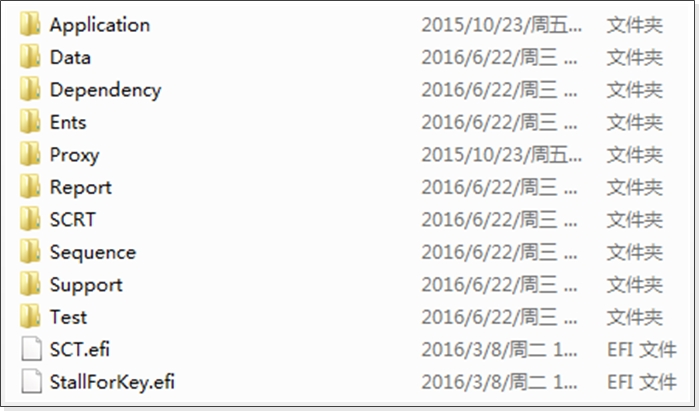
\includegraphics[height=7cm]{chart3/自动化测试工具SCT下的文件结构}
		\caption{自动化测试工具SCT下的文件结构}
		\label{fig:自动化测试工具SCT下的文件结构}
	\end{figure}
	
	\subsection{自动化测试工具的命令行控制}
	
	针对UEFI BIOS环境下对SCT的操作和控制,本文在UEFI BIOS的Shell环境下设计和实现了一个小型的命令行处理功能环境,在计算机开机但还未进入OS的情况下,用户可以通过键盘选择进入UEFI BIOS Shell命令行处理程序,在该环境下对SCT进行操作和控制。Shell是 UEFI BIOS特有的命令解析器,存在于 UEFI BIOS 中,是功能齐全的执行和调试环境用于在UEFI BIOS中进行各种设置和操作。
	
	最终实现的SCT在UEFI BIOS的Shell环境中运行。重启 PC,进入到UEFI BIOS Shell 命令行下,进入到自动化测试工具所在的目录,即可通过命令加参数运行对该工具进行操作。如图~\ref{fig:SCT-without-Parameters-Screen-Display-Using-the-Command-Line-Interface}、表~\ref{tab:自动化测试工具SCT的参数列表}所示:
	
	\begin{figure}[H] % use float package if you want it here
		\centering
		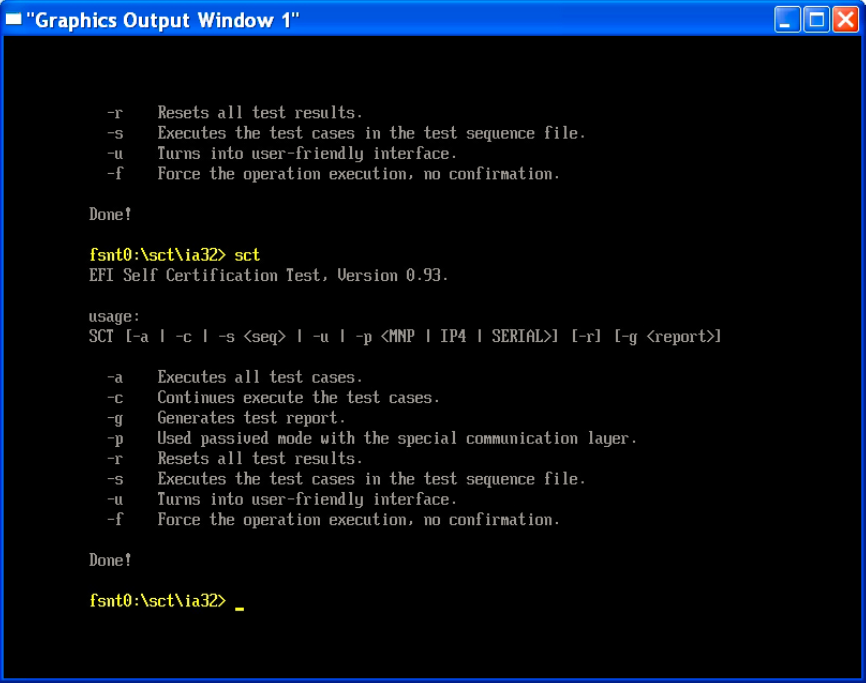
\includegraphics[height=8cm]{chart3/SCT-without-Parameters-Screen-Display-Using-the-Command-Line-Interface}
		\caption{使用命令行对SCT进行操作}
		\label{fig:SCT-without-Parameters-Screen-Display-Using-the-Command-Line-Interface}
	\end{figure}
	
	\begin{table}[H]
		\centering
		\caption{自动化测试工具SCT的参数列表}
		\label{tab:自动化测试工具SCT的参数列表}
		\begin{center}
		\begin{tabular}{|l|p{9cm}|} 
		\hline
		参数 & 描述 \\ \hline
		-a & 执行测试工具识别到的所有用例 \\ \hline
		-c & 继续执行进行中剩余未执行的用例 \\ \hline
		-g report & 生成.CSV格式的测试报告 \\ \hline
		-r & 重置测试环境以进行一轮新的测试  \\ \hline
		-s seq & 执行seq文件中指定的用例 \\ \hline
		-u & 启动测试工具进入到其主界面 \\ \hline
		-f & 不需要用户进行确认,强制执行测试操作 \\ \hline
		\end{tabular}
		\end{center}
	\end{table}
	
	\subsection{自动化测试工具的主界面}
		
		Shell环境输入命令SCT –u即可开始调用SCT的主界面,如图~\ref{fig:Main-Menu-Screen-Using-the-Menu-Driven-Interface}所示:
		
		\begin{figure}[H] % use float package if you want it here
			\centering
			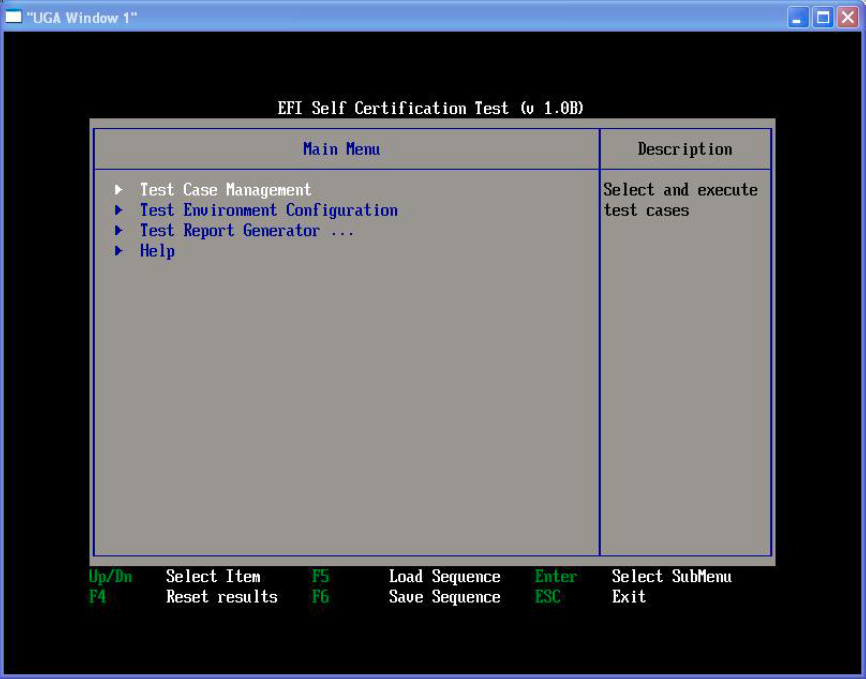
\includegraphics[height=8cm]{chart3/Main-Menu-Screen-Using-the-Menu-Driven-Interface}
			\caption{SCT的主界面菜单}
			\label{fig:Main-Menu-Screen-Using-the-Menu-Driven-Interface}
		\end{figure}
		
		主界面分为四个部分:
		
		\begin{itemize}
			\item 用例管理部分:用于在菜单中选择需要运行的用例,从而选择性的运行所需的用例。
			\item 测试环境的设置部分:通过修改测试环境的配置信息来控制其设置。
			\item 测试报告生成部分:用户利用其可以产生CSV格式的报告,并且存放到自动化测试工具主目录的Report目录中方便用户查看。
			\item 帮助信息部分。
		\end{itemize}
		
		此外在自动化测试工具的界面下可以使用快捷键方便用户操作,如表~\ref{tab:自动化测试工具SCT主界面的快捷键}所示:
		
		\begin{table}[H]
			\centering
			\caption{自动化测试工具SCT主界面的快捷键}
			\label{tab:自动化测试工具SCT主界面的快捷键}
			\begin{center}
			\begin{tabular}{|l|l|p{10cm}|} 
			\hline
			快捷键 & 功能 & 功能描述 \\ \hline
			F4 & 重置结果 & 重置所有的测试结果 \\ \hline
			F5 & 导入序列 & 从储存设备中导入测试序列文件,这一功能允许用户导入、编辑和执行现有的测试序列文件 \\ \hline
			F6 & 导出序列 & 将用户指定需要执行的用例的序列保存到一个文件 \\ \hline
			F8 & 继续执行 & 继续执行进行中剩余未执行的用例 \\ \hline
			F9 & 执行 & 执行测试工具识别到的所有用例 \\ \hline
			\end{tabular}
			\end{center}
		\end{table}
\begin{itemize}
	\item SCT的测试环境管理
		
		SCT的测试环境管理如图~\ref{fig:Test-Environment-Configuration}所示:	
		
		\begin{figure}[htbp] % use float package if you want it here
			\centering
			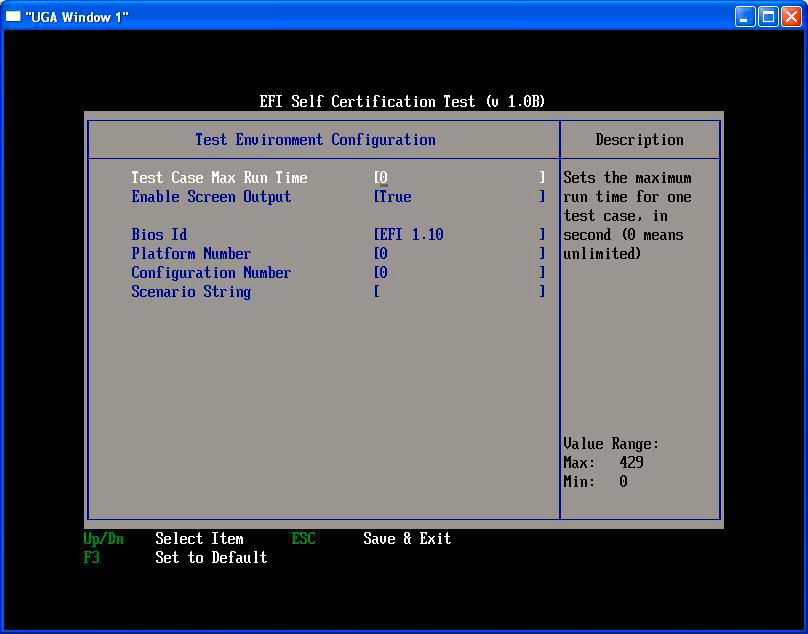
\includegraphics[height=8cm]{chart3/Test-Environment-Configuration}
			\caption{测试环境配置界面}
			\label{fig:Test-Environment-Configuration}
		\end{figure}
		
	\item SCT的用例管理
	
		SCT的用例配置管理界面主要是用来对用例进行控制和管理,如图~\ref{fig:Test-Case-Management-Screen}、~\ref{fig:Run-Time-Services-Screen}、~\ref{fig:使用seq测试序列文件来管理所需执行的测试用例}所示:
		
		\begin{figure}[H] % use float package if you want it here
			\centering
			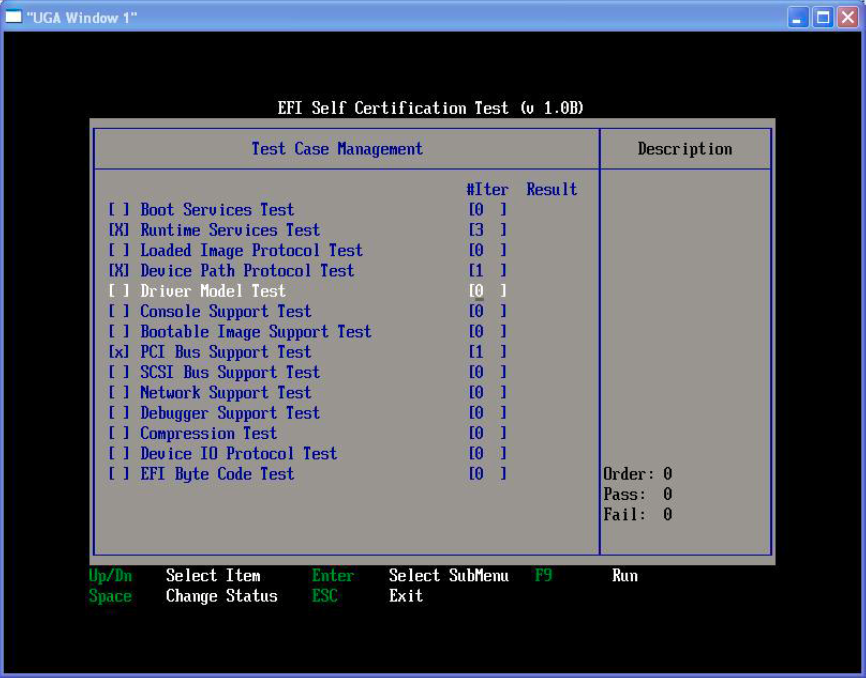
\includegraphics[height=8cm]{chart3/Test-Case-Management-Screen}
			\caption{用例管理界面}
			\label{fig:Test-Case-Management-Screen}
		\end{figure}
		
		\begin{figure}[H] % use float package if you want it here
			\centering
			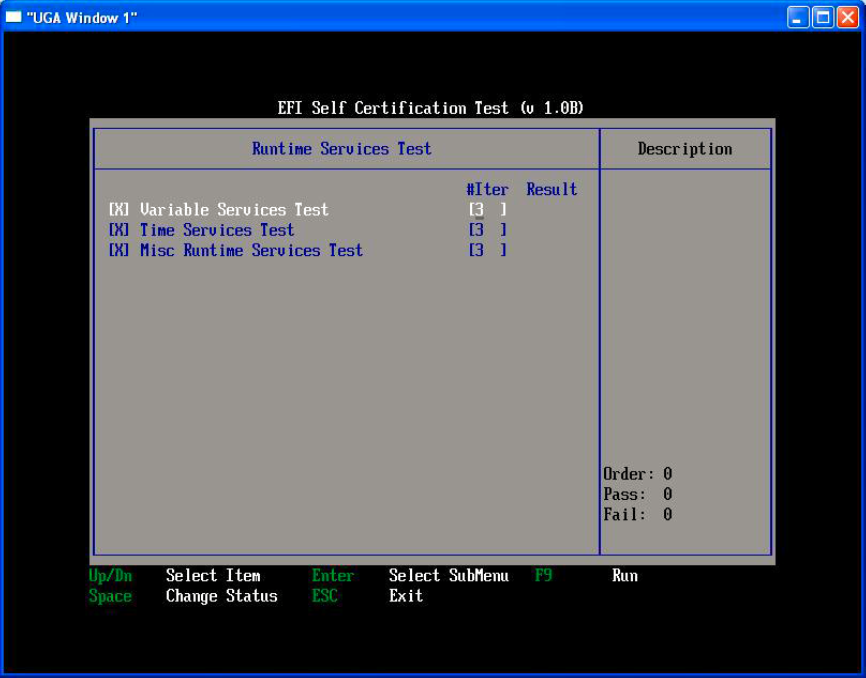
\includegraphics[height=8cm]{chart3/Run-Time-Services-Screen}
			\caption{用例执行次数管理界面}
			\label{fig:Run-Time-Services-Screen}
		\end{figure}
		
		\begin{figure}[H] % use float package if you want it here
			\centering
			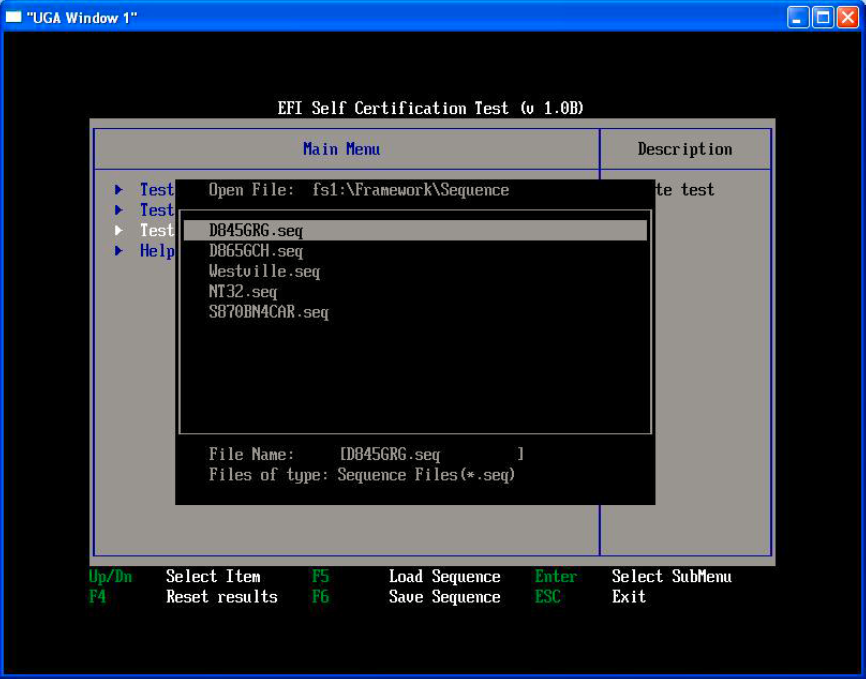
\includegraphics[height=8cm]{chart3/使用seq测试序列文件来管理所需执行的测试用例}
			\caption{使用seq测试序列文件来管理所需执行的测试用例}
			\label{fig:使用seq测试序列文件来管理所需执行的测试用例}
		\end{figure}
	
	\item SCT的测试报告生成器
	
		SCT的测试报告生成器主要用于对已执行完的日志和结果进行分析和总结,生成相应的测试报告。如图~\ref{fig:生成csv格式的测试报告}所示:
	
		\begin{figure}[H] % use float package if you want it here
			\centering
			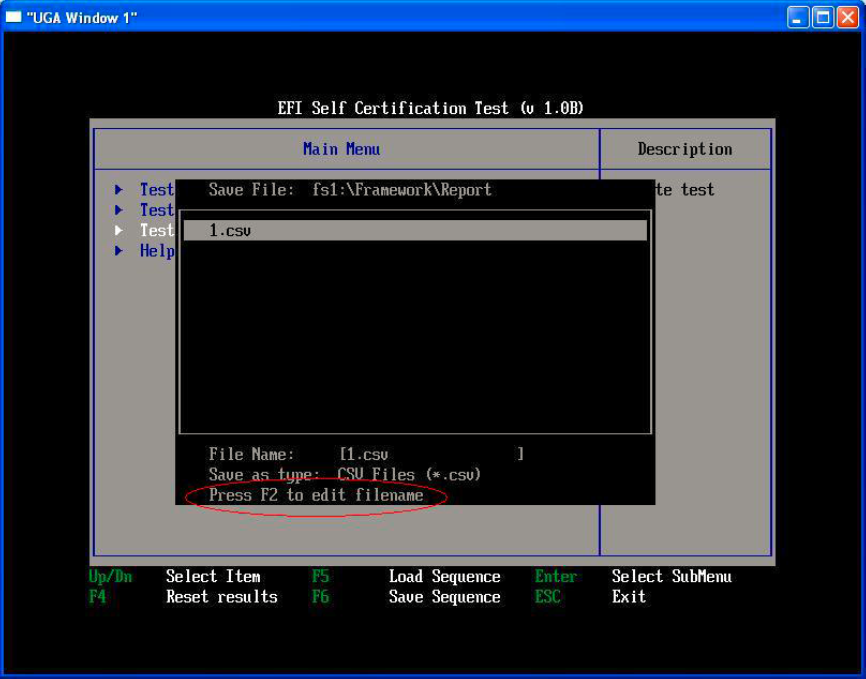
\includegraphics[height=8cm]{chart3/生成csv格式的测试报告}
			\caption{生成csv格式的测试报告}
			\label{fig:生成csv格式的测试报告}
		\end{figure}
		
\end{itemize}	
		
	\subsection{自动化测试工具的测试日志与报告}
	
		每一个用例在执行时,会自动将测试的进展情况写入到相应的日志文件中并且储存到测试工具主目录下对应的子目录中。每一个测试点都会相应对测试的结果进行记录,即Pass或者Failure。日志文件分为.log和.ekl两种不同类型的格式。.log日志文件是可读的文件,.ekl是供报告生成器分析的日志文件,两者仅在格式上有所区别。在所有的用例执行完成后,测试工具自带的报告生成器会解析其所有的.ekl文件,依据测试结果进行归类统计生成最后的CSV格式报表。CSV格式的文件在都有相应的软件可以打开,QA只需查看CSV中的信息便可了解此轮UEFI BIOS测试的结果。如图~\ref{fig:测试日志}、~\ref{fig:csv格式的测试报告可以使用Excel进行访问}所示:
		
		\begin{figure}[H] % use float package if you want it here
			\centering
			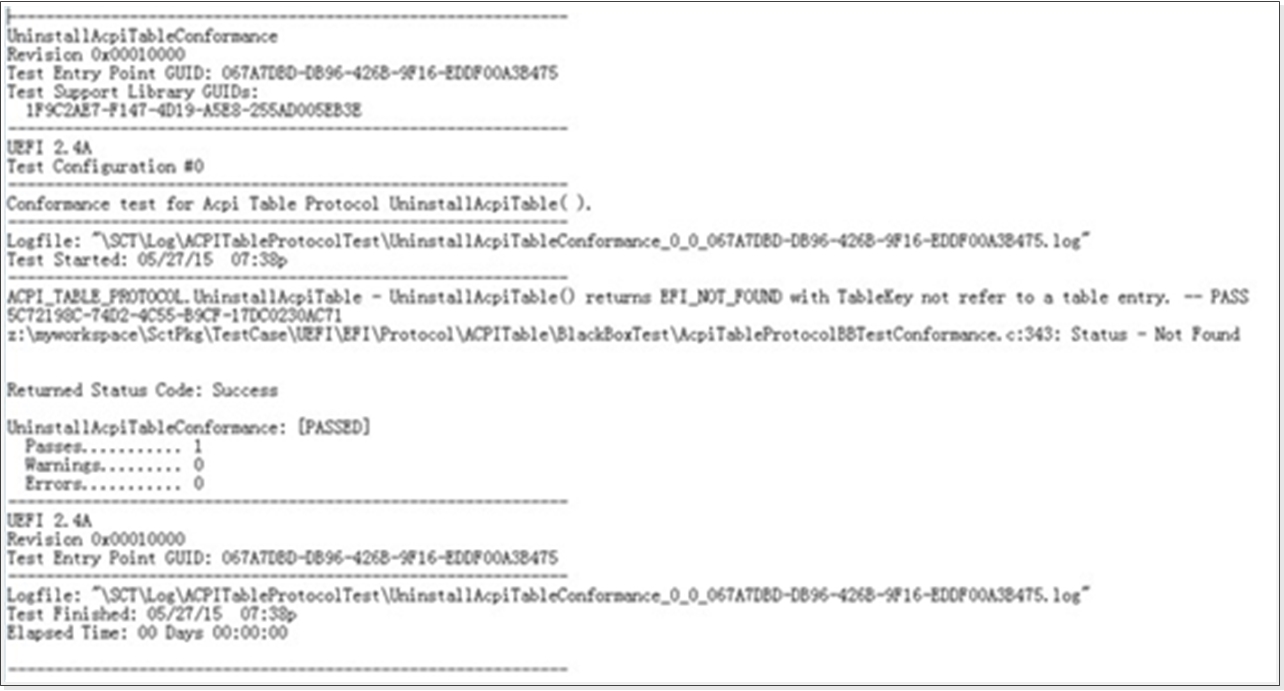
\includegraphics[height=7.5cm]{chart3/测试日志}
			\caption{测试日志}
			\label{fig:测试日志}
		\end{figure}
		
		\begin{figure}[H] % use float package if you want it here
			\centering
			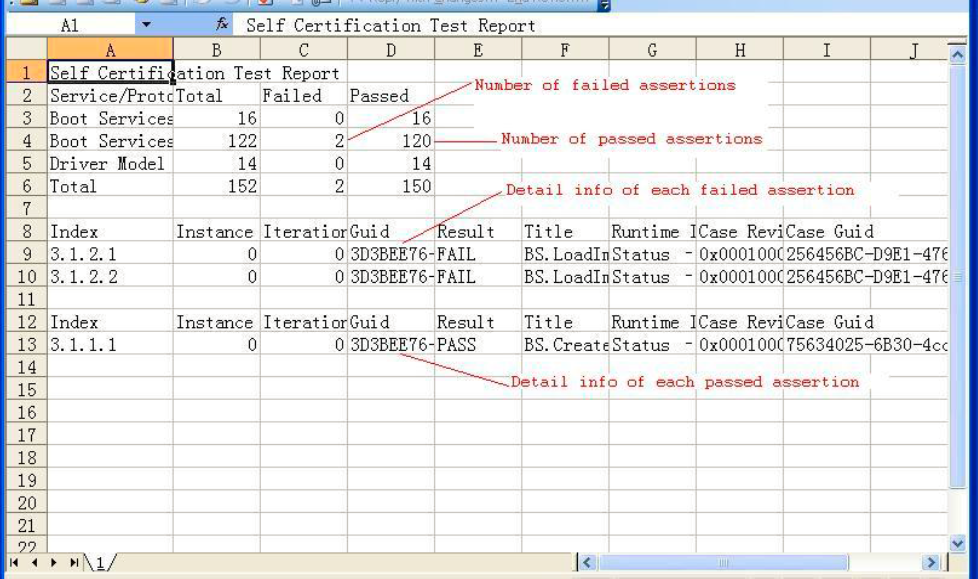
\includegraphics[height=8cm]{chart3/csv格式的测试报告可以使用Excel进行访问}
			\caption{csv格式的测试报告可以使用Excel进行访问}
			\label{fig:csv格式的测试报告可以使用Excel进行访问}
		\end{figure}
	
\section{本章小结}
   	
	本章主要分析了UEFI BIOS持续集成测试系统中所需的测试工具SCT的设计,并且对其进行了实现。通过明确SCT的设计目标、对其进行需求分析,初步得出了其系统功能组成和系统功能流程,并且进一步对其进行具体设计与实现,最后讲述该自动化测试工具的使用方法,以便于后续UEFI BIOS持续集成测试系统中对该工具的使用。
	
	目前SCT已成功实现并且通过验证,应用于UEFI BIOS的测试工作,即便是没有代码经验的QA也能方便、快捷、高质量的使用其完成对UEFI BIOS产品质量的自动化测试工作,在产品的不断迭代与更新中起到了非常重要的效果和应用价值。

	
\chapter{Denlow-X64持续集成测试系统的设计与实现}
\label{cha:intro}

\section{Denlow-X64的背景介绍}

Denlow是以VS2013提供的库为函数库进行编写的一种平台的UEFI BIOS,其编译生成的二进制文件大小为16MB,可以烧录到真实普通PC环境下主板的ROM芯片中以供计算机使用。

在本章中,我们以Denlow平台为例,说明在该种平台下的持续集成测试系统的搭建。最终的完成目标是:在X-64架构(特定的CPU架构)的Denlow平台上,实现对该种架构的UEFI BIOS平台持续集成测试系统的搭建,并且应用到Denlow-X64的实际开发项目中去。

\section{Denlow-X64持续集成测试系统的设计方案}
	\subsection{Denlow-X64持续集成测试系统的环境组成}
		
		Denlow-X64持续集成测试系统的环境组成如图~\ref{fig:Denlow-X64持续集成测试系统的环境组成}所示:
		
		\begin{figure}[H] % use float package if you want it here
			\centering
			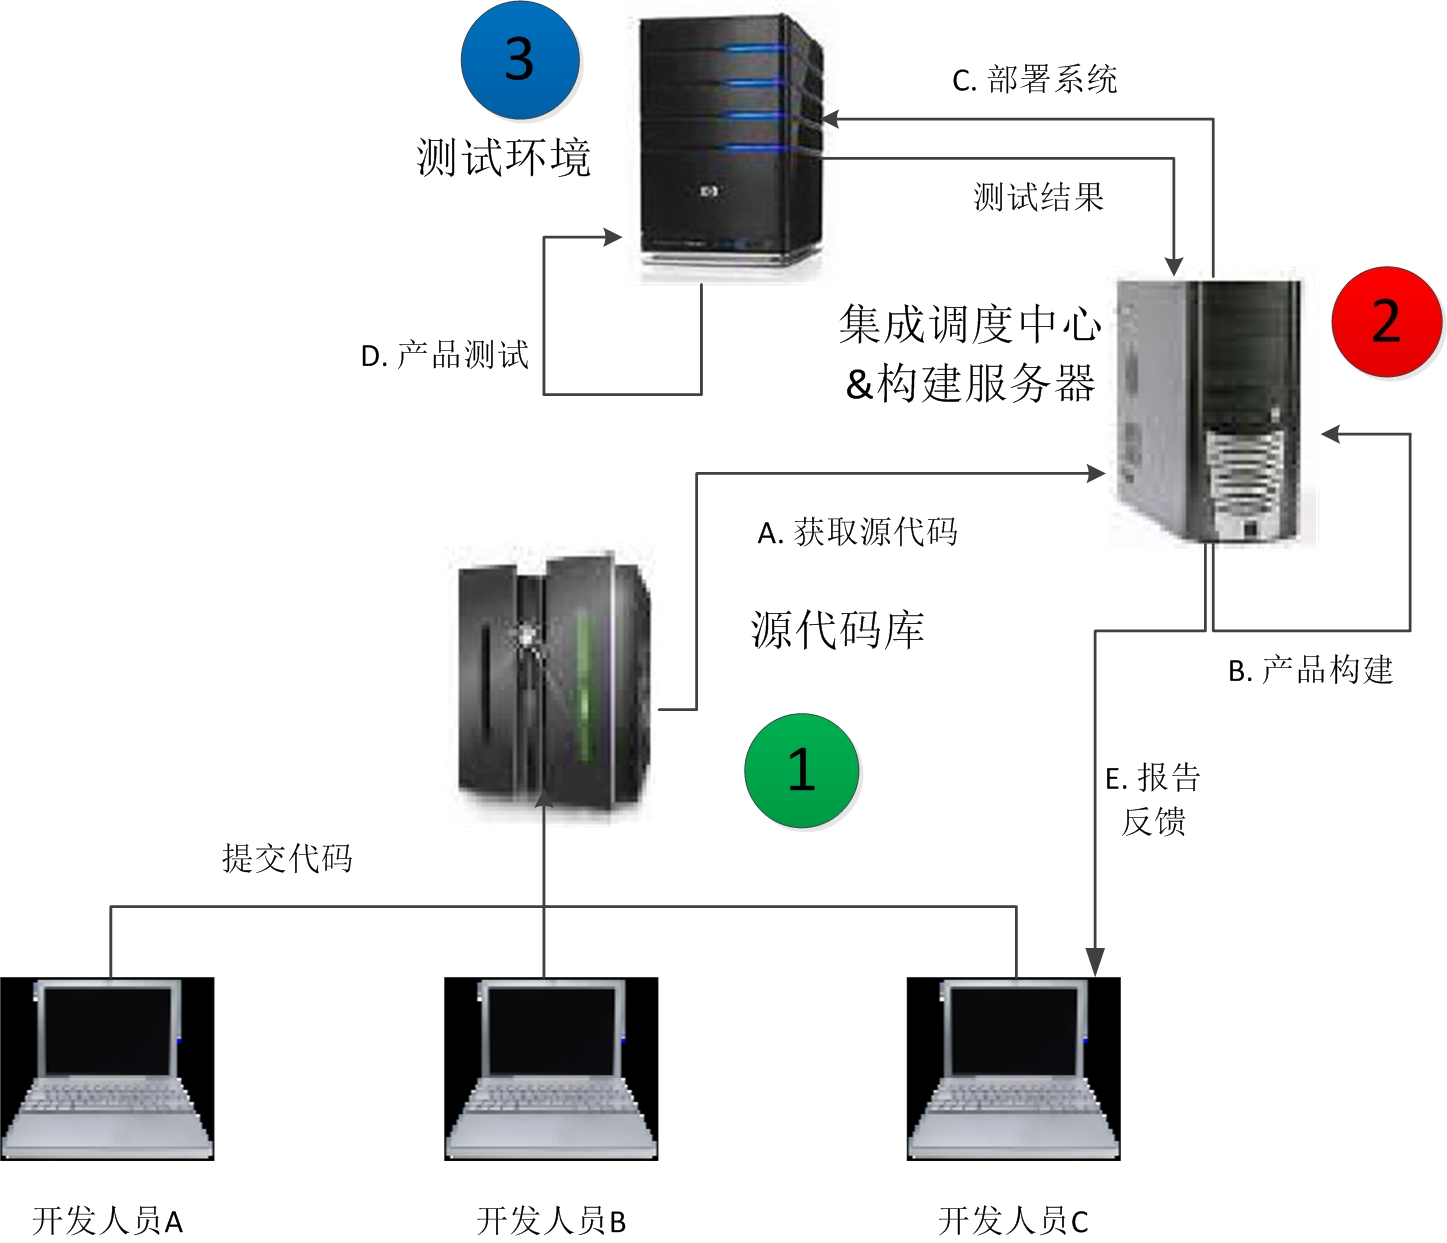
\includegraphics[height=10cm]{chart4/Denlow-X64持续集成测试系统的环境组成}
			\caption{Denlow-X64持续集成测试系统的环境组成}
			\label{fig:Denlow-X64持续集成测试系统的环境组成}
		\end{figure}
		
		其环境主要由源代码库、集成调度中心(同时也是产品构建服务器)和测试环境三部分组成。
		
		\begin{itemize}
			\item 源代码库
			
				源代码库主要负责存储管理Denlow-X64产品的源文件,以便于后续构建服务器对其进行获取和编译构建成所需要的产品进行测试工作。
			\item 集成调度中心(同时也是构建服务器)
				
				集成调度中心主要负责对该持续集成测试系统各功能部分进行调度,例如:
					\begin{itemize}
						\item 通过源代码库下载Denlow-X64的源代码。
						\item 编译构建产品。
						\item 解析测试机端的测试结果。
						\item 报告反馈。
					\end{itemize}
			\item 测试环境
				
				测试环境主要负责测试环境的部署以及对Denlow-X64利用SCT执行功能性测试。
		\end{itemize}
	
	\subsection{Denlow-X64 持续集成测试系统的功能组成}
		
		Denlow-X64持续集成测试系统功能框架组成如图~\ref{fig:Denlow-X64持续集成测试系统的功能框架组成}所示:
		
		\begin{figure}[H] % use float package if you want it here
			\centering
			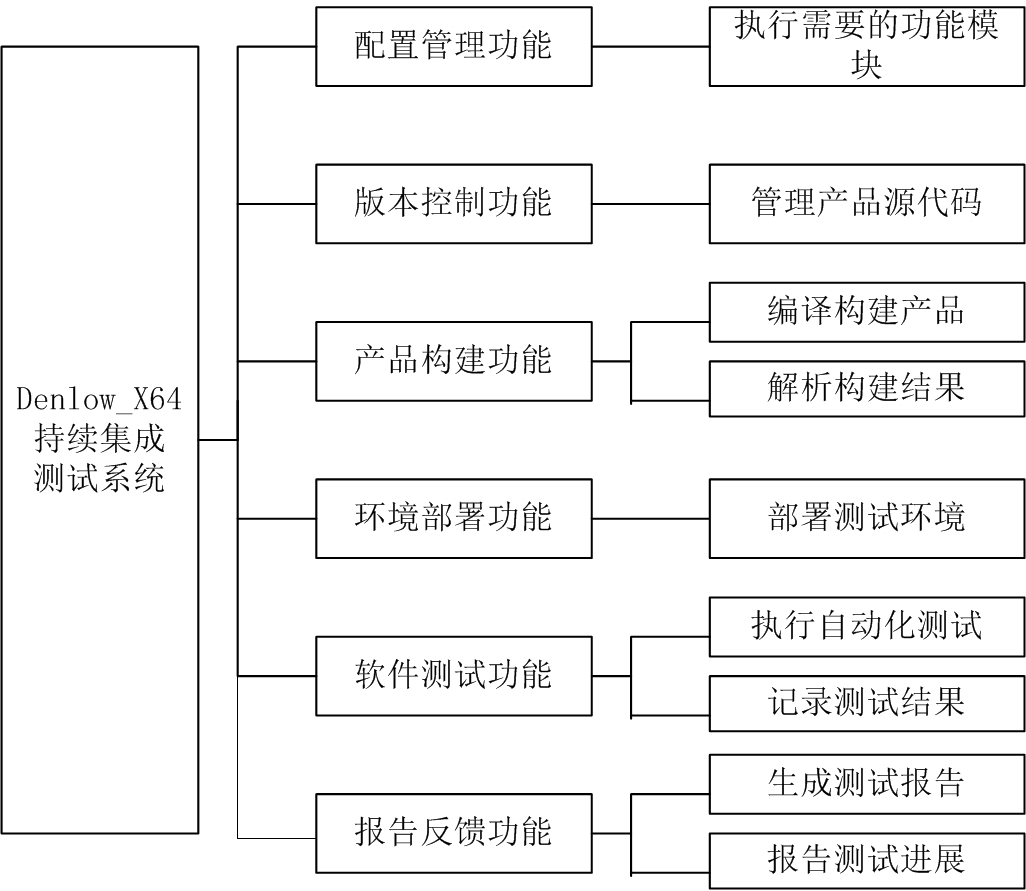
\includegraphics[height=9cm]{chart4/Denlow-X64持续集成测试系统的功能框架组成}
			\caption{Denlow-X64持续集成测试系统的功能框架组成}
			\label{fig:Denlow-X64持续集成测试系统的功能框架组成}
		\end{figure}
		
		其功能框架主要由:1)配置管理功能;2)版本控制功能;3)产品构建功能;4)环境部署功能;5)软件测试功能;6)报告反馈功能六部分模块组成。
	
	\subsection{Denlow-X64 持续集成测试系统的功能流程}
		
		Denlow-X64持续集成测试系统的功能流程如图~\ref{fig:Denlow-X64持续集成测试系统的功能流程}所示:
		
		\begin{figure}[H] % use float package if you want it here
			\centering
			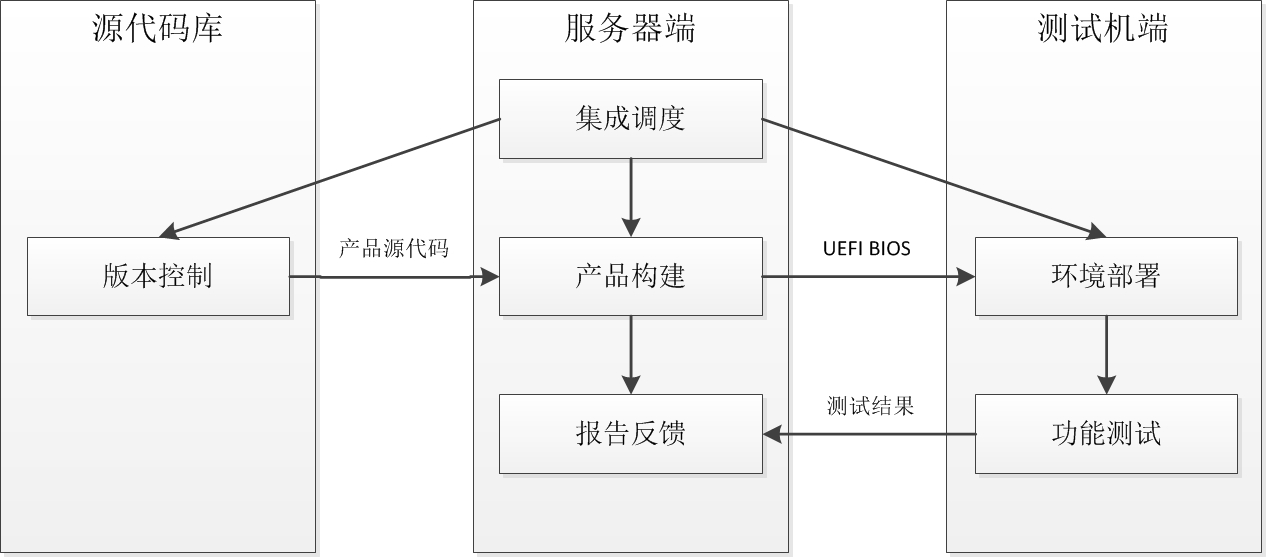
\includegraphics[height=6cm]{chart4/Denlow-X64持续集成测试系统的功能流程}
			\caption{Denlow-X64持续集成测试系统的功能流程}
			\label{fig:Denlow-X64持续集成测试系统的功能流程}
		\end{figure}
		
		服务器负责对整个持续集成测试系统的进行集成调度,其通过版本控制系统从源代码库中获取源文件进行产品构建,将其部署到测试机的环境中,之后利用SCT对产品进行功能性测试,并且将其结果报告、反馈给相关的项目组成员。 

\section{Denlow-X64持续集成测试系统各组成模块的设计与实现}
	
	Denlow-X64持续集成测试系统主要由配置管理、版本控制、产品构建、环境部署、软件测试功能和报告反馈六个模块组成。
	
	由于测试机的操作系统为Windows 2007,服务器的操作系统为Windows Server 2008,测试环境部署以及软件测试需要在测试机UEFI BIOS Shell中进行,因此我们最终选用Windows DOS$\backslash$BAT脚本与UEFI BIOS Shell脚本对该系统进行最终实现。
	
	\subsection{配置管理模块的设计与实现}
		
		为了方便管理Denlow-X64持续集成测试系统各模块是否执行,因此设计和实现本模块用于对系统进行配置和管理。配置文件中的配置信息的设计如图~\ref{fig:配置文件中配置信息的设计}所示:
		
		\begin{figure}[H] % use float package if you want it here
			\centering
			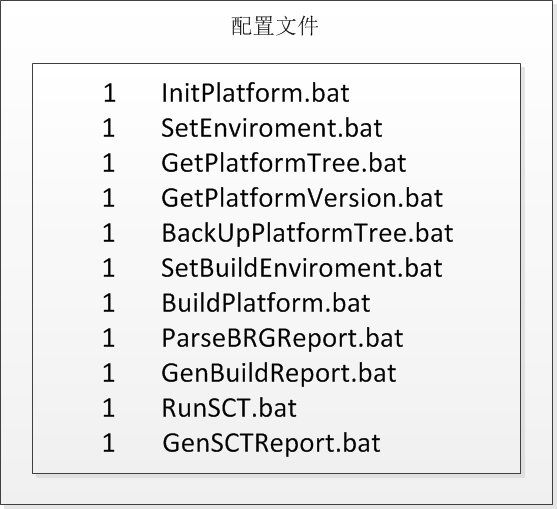
\includegraphics[height=6.5cm]{chart4/配置文件中配置信息的设计}
			\caption{配置文件中配置信息的设计}
			\label{fig:配置文件中配置信息的设计}
		\end{figure}
		
		该配置文件放置在系统主文件夹下的CallingTable.txt文件当中。系统启动之前测试人员对配置文件进行配置,通过修改该配置文件中的内容完成对其的管理:将配置文件中需要执行的模块设置为1,不需要执行的模块设置为0。系统启动时会先解析该配置文件获取相关配置信息,根据其决定所需要执行的模块。如图~\ref{fig:Denlow-X64持续集成测试系统配置管理模块的设计}所示:
		
		\begin{figure}[H] % use float package if you want it here
			\centering
			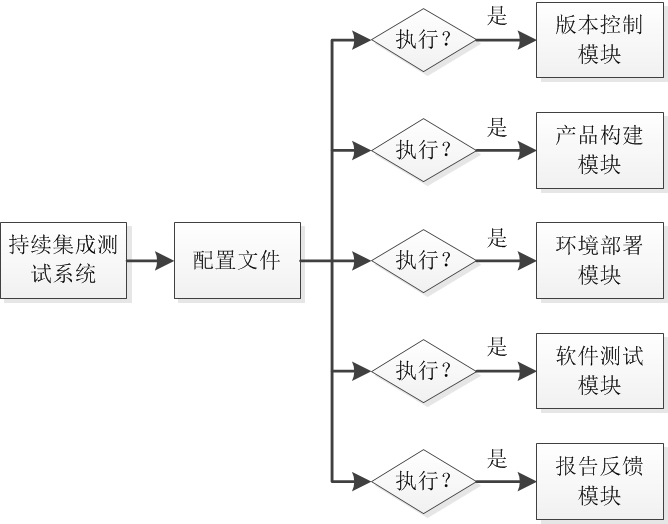
\includegraphics[height=8.5cm]{chart4/Denlow-X64持续集成测试系统配置管理模块的设计}
			\caption{Denlow-X64持续集成测试系统配置管理模块的设计}
			\label{fig:Denlow-X64持续集成测试系统配置管理模块的设计}
		\end{figure}
		
		该模块的主要由main.bat实现,持续集成测试系统启动时首先执行main.bat,进入运行界面,读取配置文件中的配置内容,依次执行配置信息设置为1的各模块脚本,从而实现配置管理模块所需要实现的功能。其中系统的运行界面如图~\ref{fig:Denlow-X64持续集成测试系统集成调度中心的运行界面}所示:
			
		\begin{figure}[H] % use float package if you want it here
			\centering
			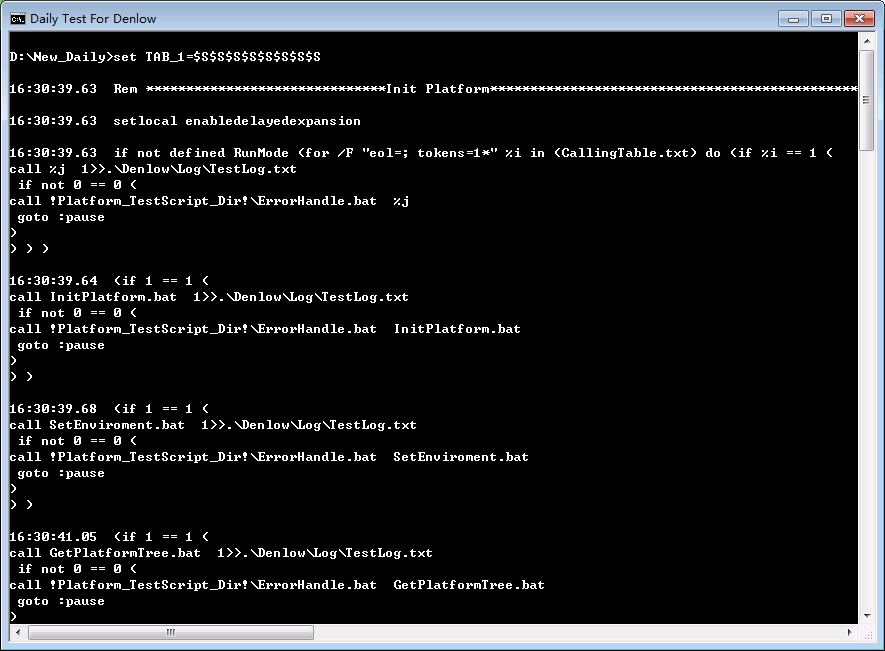
\includegraphics[height=8cm]{chart4/Denlow-X64持续集成测试系统集成调度中心的运行界面}
			\caption{Denlow-X64持续集成测试系统集成调度中心的运行界面}
			\label{fig:Denlow-X64持续集成测试系统集成调度中心的运行界面}
		\end{figure}
	
	\subsection{版本控制模块的设计与实现}
		版本控制模块主要用于管理项目源文件、获取源文件便于后续利用其进行产品构建、获取源文件版本号用于产品构建报告、备份获取到的源文件,其中所用的版本控制系统为Subversion(SVN)。其功能流程如~\ref{fig:Denlow-X64持续集成测试系统版本控制模块的设计}所示:
		
		\begin{figure}[H] % use float package if you want it here
			\centering
			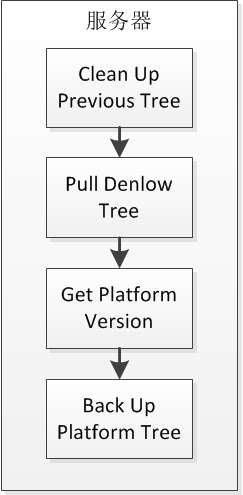
\includegraphics[height=6.5cm]{chart4/Denlow-X64持续集成测试系统版本控制模块的设计}
			\caption{Denlow-X64持续集成测试系统版本控制模块的设计}
			\label{fig:Denlow-X64持续集成测试系统版本控制模块的设计}
		\end{figure}
		
		该模块的主要由三部分脚本共同实现:
		
		\begin{itemize}
			\item GetPlatformTree.bat
			
				GetPlatformTree.bat主要用于:1. Clean Up Previous Tree。2. Pull Denlow Tree。
				\begin{itemize}
					\item Clean Up Previous Tree主要用于清除上一次系统运行时从源代码库中下载的源代码。其先判断源代码文件夹存在与否,若是则删除前一次系统运行时下载的旧版本源文件。
					\item Pull Denlow Tree主要用于利用SVN从源代码库中获取最新版本的源文件。其首先利用SVN从源代码库中尝试获取源文件,若获取成功则结束本脚本执行下一脚本;否则需要利用SVN从源代码库中获取源文件。若该部分执行60次后仍然未能正常获取到产品源文件,则系统获取源文件失败并且结束本部分功能。失败原因可能是由于网络不可用、SVN服务器宕机等非系统因素。
				\end{itemize}
			\item GetPlatformVersion.bat
			
				GetPlatformVersion.bat主要用来获取EDK2和Denlow的版本号等信息,用于后续报告反馈模块。其通过SVN获取EDK2版本号和Denlow的版本号将其赋予相应变量,以便于后续模块对其进行使用。
			\item BackUpPlatformTree.bat
			
				BackUpPlatformTree.bat用于将获取的产品源文件进行备份。
		\end{itemize}
	
	\subsection{产品构建模块的设计与实现}
		
		产品构建模块主要功能是将Denlow-X64的源文件编译构建成为当前版本的UEFI BIOS 产品Denlow.fd,并且生成相应的产品构建报告。其功能流程如图~\ref{fig:Denlow-X64持续集成测试系统产品构建模块的设计}所示:
		
		\begin{figure}[H] % use float package if you want it here
			\centering
			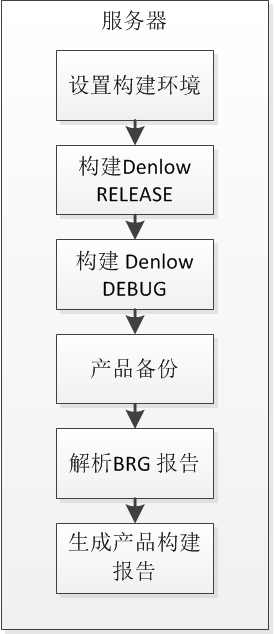
\includegraphics[height=7cm]{chart4/Denlow-X64持续集成测试系统产品构建模块的设计}
			\caption{Denlow-X64持续集成测试系统产品构建模块的设计}
			\label{fig:Denlow-X64持续集成测试系统产品构建模块的设计}
		\end{figure}
		
		该模块的主要由四部分脚本共同实现:
		
		\begin{itemize}
			\item SetBuildEnviroment.bat
				
				SetBuildEnviroment.bat用于设置构建环境以便于后续进行产品构建。SetBuildEnviroment.bat首先调用VS2013安装目录下的vcvarsx86-ia64.bat脚本以设置环境变量,之后调用Denlow源文件中的edksetup.bat脚本以设置产品默认的开发配置。
			\item BuildPlatform.bat
				
				BuildPlatform.bat主要用于编译构建产品,其需要先后构建产品X64的Release版本和Debug版本。其中Release版本的产品需要对其进行环境部署并且进行测试。Build Denlow RELEASE首先清除掉之前一次的产品构建结果与日志,之后进行产品RELEASE版本的构建。若有RELEASE版本的产品出现则判断产品RELEASE版本构建成功,将构建的产品进行备份;否则判断产品构建失败。最后将构建过程中产生的报告文件ReportFile.txt进行备份。
			
				Build Denlow DEBUG用于构建产品的DEBUG版本,判断其是否构建成功,并且对其进行备份。Build Denlow DEBUG首先进行产品DEBUG版本的构建。若有DEBUG版本的产品出现则判断产品DEBUG版本构建成功,将构建的产品进行备份;否则判断产品构建失败。最后将构建过程中产生的报告文件ReportFile.txt进行备份。
			\item ParseBRGReport.bat
				
				产品RELEASE和DEBUG版本的构建过程中会分别产生report-DenlowX64Release.txt与report-DenlowX64Debug.txt。以report-DenlowX64Release.txt为例,其文件头部如图~\ref{fig:report-DenlowX64Release}所示:
				
				\begin{figure}[H] % use float package if you want it here
					\centering
					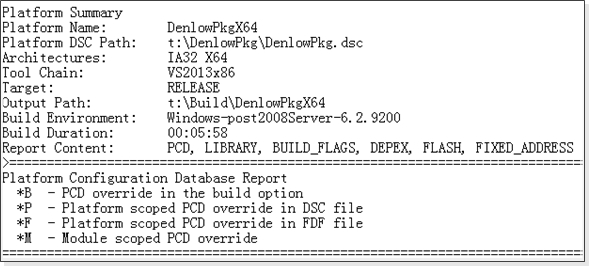
\includegraphics[height=5.5cm]{chart4/report-DenlowX64Release}
					\caption{report-DenlowX64Release}
					\label{fig:report-DenlowX64Release}
				\end{figure}
				
				文件中的Report Content对每一个BRG session进行了总结,ParseBRGReport.bat主要功能是解析该文件,根据Report Content中的session判断每一个BRG session是否正确,并且对判断结果以HTML格式的语句进行记录,如图~\ref{fig:build-results}所示:
				
				\begin{figure}[H] % use float package if you want it here
					\centering
					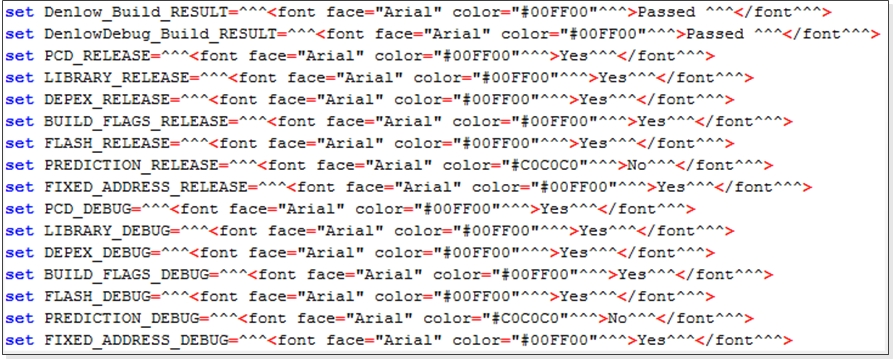
\includegraphics[height=5.5cm]{chart4/build-results}
					\caption{build-results}
					\label{fig:build-results}
				\end{figure}
				
			\item GenBuildReport.bat
				
				GenBuildReport.bat主要依据之前BuildPlatform.bat过程的构建结果判断记录以及ParseBRGReport.bat对BRG session的解析结果,生成网页格式的构建报告以方便QA查看产品构建的结果。其功能流程如图~\ref{fig:GenDenlowBuildReport的功能流程图}所示:
				
				\begin{figure}[H] % use float package if you want it here
					\centering
					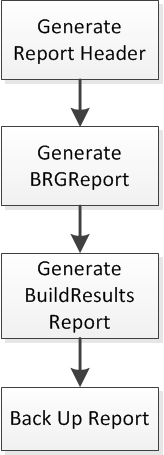
\includegraphics[height=6.5cm]{chart4/GenBuildReport的功能流程图}
					\caption{GenBuildReport的功能流程图}
					\label{fig:GenDenlowBuildReport的功能流程图}
				\end{figure}
				
				GenBuildReport.bat首先生成报告头部,之后依据BRG解析的结果生成报告中BRG报告的相应部分,之后依据之前产品构建结果生成报告中的产品构建的相应部分,最后将整个生成的报告进行备份。
		\end{itemize}
		
	\subsection{环境部署模块的设计与实现}
		
		环境部署模块的主要功能是将之前构建成功的Release版本的UEFI BIOS产品Denlow.fd烧录到测试机主板的ROM芯片中,完成测试环境的部署以便于后续系统对产品的测试。其功能流程如图~\ref{fig:Denlow-X64持续集成测试系统环境部署模块的设计}所示:
		
		\begin{figure}[H] % use float package if you want it here
			\centering
			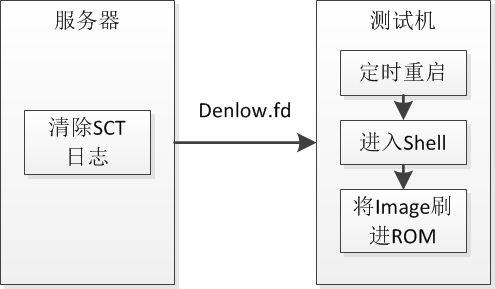
\includegraphics[height=5cm]{chart4/Denlow-X64持续集成测试系统环境部署模块的设计}
			\caption{Denlow-X64持续集成测试系统环境部署模块的设计}
			\label{fig:Denlow-X64持续集成测试系统环境部署模块的设计}
		\end{figure}
		
		该模块功能主要由服务器的脚本RunSCT.bat与测试机端脚本的Startup.nsh共同实现。
		
		\begin{itemize}
			\item Windows映射网络驱动器
				
				为了便于在同一局域网下的服务器和测试机之间传递文件,需要利用Windows映射网络驱动器技术将测试机的共享文件夹映射为服务器的一个映射盘。其设置如图~\ref{fig:利用Windows映射网络驱动器实现文件夹映射}所示:
			
				\begin{figure}[H] % use float package if you want it here
					\centering
					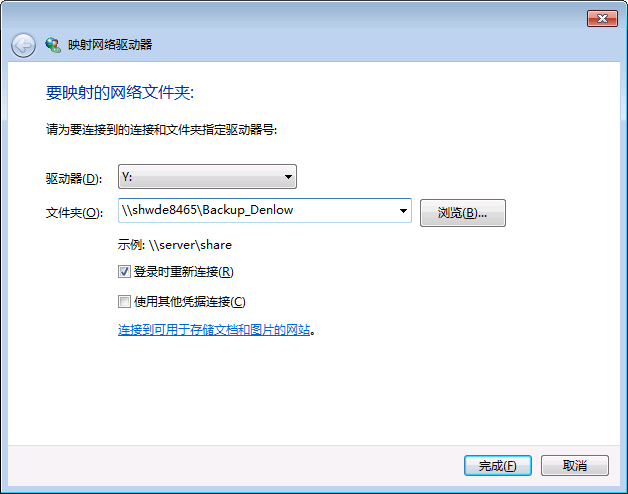
\includegraphics[height=8cm]{chart4/利用Windows映射网络驱动器实现文件夹映射}
					\caption{利用Windows映射网络驱动器实现文件夹映射}
					\label{fig:利用Windows映射网络驱动器实现文件夹映射}
				\end{figure}
			
			\item RunDenlowSCT.bat
				
				RunDenlowSCT.bat用于清除系统上一次执行时的SCT日志,并且将需要测试的产品拷贝到测试机以便于测试机对其进行部署。其功能流程如图~\ref{fig:RunDenlowSCT的功能流程图}所示:
				
				\begin{figure}[H] % use float package if you want it here
					\centering
					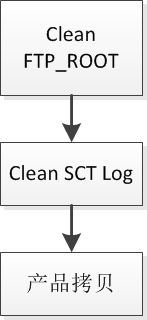
\includegraphics[height=5cm]{chart4/RunDenlowSCT的功能流程图}
					\caption{RunDenlowSCT.bat的功能流程图}
					\label{fig:RunDenlowSCT的功能流程图}
				\end{figure}
				
				Clean FTP-ROOT和Clean SCT Log主要用来清除上一次集成测试时生成的日志文件,以便于后续利用SCT对产品测试时重新生成日志。
				
				Copy Image To Test Computer主要将构建好的Release版本的产品通过设置好的映射盘拷贝到测试机的硬盘中,以便于后续测试环境部署。
			\item 测试机定时重启进入UEFI BIOS Shell环境
				
				该部分主要功能是在服务器产品构建完成并且拷贝到测试机后,测试机定时重启进入UEFI BIOS Shell环境,在Shell环境下利用FirmwareUpdate.efi工具将Image烧录到测试机主板的ROM芯片中,完成测试环境的部署,以便于后续对其进行测试。值得一提的是,UEFI BIOS Shell 有自己的特性,如果计算机开机启动到UEFI BIOS Shell下,在五秒内没有任何操作,则Shell 会自动去检测计算机硬盘中是否有 startup.nsh文件,并且读取该文件中内容执行其中的命令。
				
				为了实现测试机定时重启并且进入UEFI BIOS Shell环境,需要将UEFI BIOS Shell设为开机第一位启动,并且利用Windows 任务计划设置好测试机每天固定的重启时间。定时重启的设置如图~\ref{fig:测试机利用Windows任务计划实现定时重启(一)}、~\ref{fig:测试机利用Windows任务计划实现定时重启(二)}所示:
				
				\begin{figure}[H]
					\begin{minipage}{0.48\textwidth}
					  \centering
					  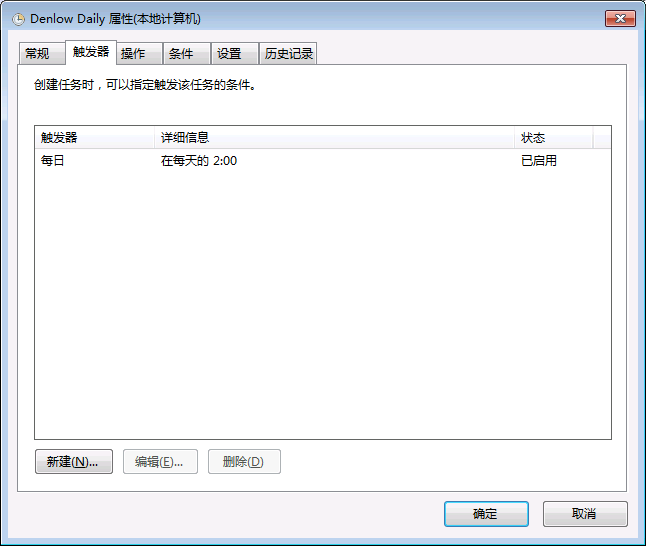
\includegraphics[height=6cm]{chart4/测试机利用Windows任务计划实现定时重启(一)}
					  \caption{测试机利用Windows任务计划实现定时重启(一)}
					  \label{fig:测试机利用Windows任务计划实现定时重启(一)}
					\end{minipage}\hfill
					\begin{minipage}{0.48\textwidth}
					  \centering
					  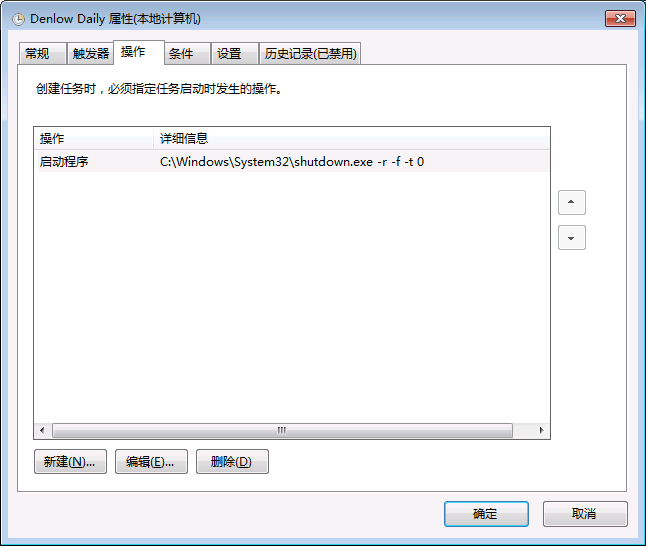
\includegraphics[height=6cm]{chart4/测试机利用Windows任务计划实现定时重启(二)}
					  \caption{测试机利用Windows任务计划实现定时重启(二)}
					  \label{fig:测试机利用Windows任务计划实现定时重启(二)}
					\end{minipage}
				\end{figure}
				
				这样测试机在每天固定时间重启,并且进入UEFI BIOS Shell环境下,读取Startup.nsh中的内容,执行其中的命令从而将Image烧录到测试机主板的ROM芯片中完成测试环境的部署。
			\item Startup.nsh
				
				Startup.nsh主要功能是利用FirmwareUpdate.efi工具将构建好的产品Denlow.fd烧录到测试机主板的ROM芯片中完成测试环境的部署。
				
				测试机首先重置自动化测试工具SCT的环境,之后利用FirmwareUpdate.efi工具将Image文件烧录到测试机主板的ROM芯片中,完成测试环境部署。
		\end{itemize}
					
	\subsection{软件测试模块的设计与实现}
		
		软件测试模块的主要功能是利用自动化测试工具SCT对已经部署好的Denlow UEFI BIOS进行测试,及时发现产品存在的缺陷。其功能流程如图~\ref{fig:Denlow-X64持续集成测试系统软件测试模块的设计}所示:
		
			\begin{figure}[H] % use float package if you want it here
				\centering
				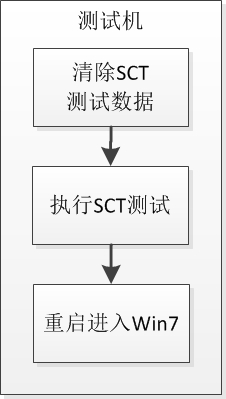
\includegraphics[height=6cm]{chart4/Denlow-X64持续集成测试系统软件测试模块的设计}
				\caption{Denlow-X64持续集成测试系统软件测试模块的设计}
				\label{fig:Denlow-X64持续集成测试系统软件测试模块的设计}
			\end{figure}
		
		自动化测试工具SCT的开发与设计已经在前面章节详细讲述,利用SCT能够实现对产品的自动化测试,并且生成相应的测试日志和初步的测试结果。系统在环境部署模块执行完毕后会重启再次进入UEFI BIOS Shell界面,读取Startup.nsh文件中的内容。因此通过将该部分的操作写入Startup.nsh文件以实现测试的自动化。
	
	\subsection{报告反馈模块的设计与实现}
		
		报告反馈模块的主要功能是在产品构建失败时及时通过邮件向测试人员反馈,以帮助测试人员及时发现问题,并且解析SCT测试的结果,生成相应的报告。其功能流程如图~\ref{fig:报告反馈模块的功能流程图}所示:
		
			\begin{figure}[H] % use float package if you want it here
				\centering
				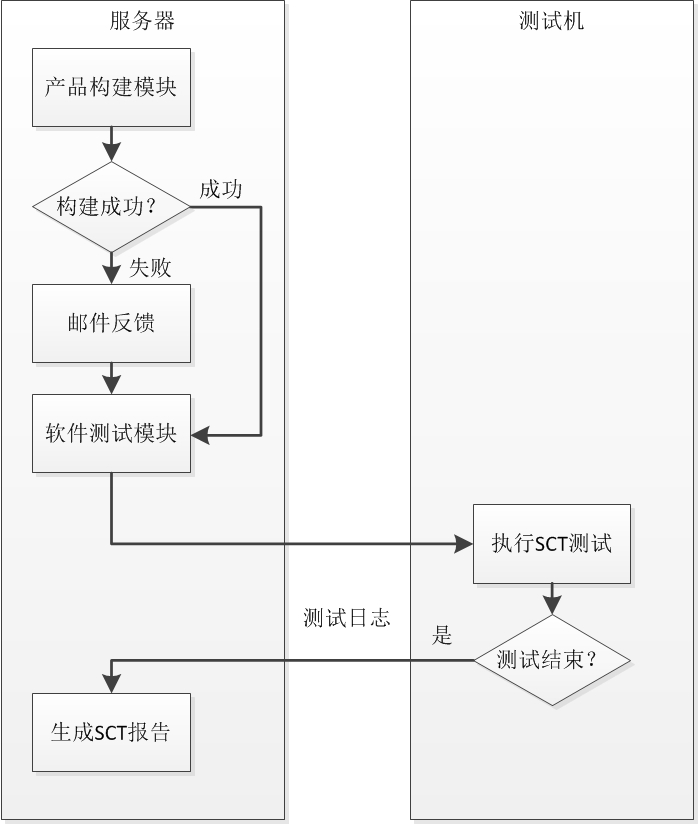
\includegraphics[height=10cm]{chart4/报告反馈模块的功能流程图}
				\caption{报告反馈模块的功能流程图}
				\label{fig:报告反馈模块的功能流程图}
			\end{figure}
		
		该部分的实现主要由MailNotify.bat与GenDenlowSCTReport.bat两部分组成。
		
		\begin{itemize}
			\item MailNotify.bat
				
				MailNotify.bat主要功能是在产品构建失败时及时反馈给测试人员。MailNotify.bat通过SendMail.bat调用已经配置好的SendEmail.exe将产品构建失败的主题和内容通过邮件及时反馈给测试人员,帮助QA快速察觉系统存在的问题,以保障测试活动的顺利开展。
			\item GenDenlowSCTReport.bat
				
				GenDenlowSCTReport.bat负责监测测试机上的SCT测试是否完成,完成后对测试结果进行总结并且生成HTML格式的测试报告,及时报告测试的结果以及产品中存在的缺陷。其功能流程如图~\ref{fig:GenDenlowSCTReport的功能流程图}所示:
				
				\begin{figure}[H] % use float package if you want it here
					\centering
					\includegraphics[height=8.5cm]{chart4/GenDenlowSCTReport的功能流程图}
					\caption{GenDenlowSCTReport的功能流程图}
					\label{fig:GenDenlowSCTReport的功能流程图}
				\end{figure}
				
				测试工具SCT完成对UEFI BIOS的测试需要几个小时的时间运行,因此需要以30分钟为单元对测试是否结束进行判断,若测试未完成则休眠30分钟;否则测试结束,利用之前介绍的文件夹映射将测试机上的测试日志拷贝到服务器中,对其进行解析,并且最终生成HTML格式的测试报告,完成系统该轮持续集成所有的任务。
		\end{itemize}
	
	\subsection{系统日志模块的设计与实现}
		
		系统日志模块的主要功能是在系统运行时对其进展进行记录,以帮助系统运行出错时测试人员能够尽快找到原因解决问题。其设计如图~\ref{fig:Denlow-X64持续集成测试系统日志模块的设计}所示:
		
			\begin{figure}[H] % use float package if you want it here
				\centering
				\includegraphics[height=8cm]{chart4/Denlow-X64持续集成测试系统日志模块的设计}
				\caption{Denlow-X64持续集成测试系统日志模块的设计}
				\label{fig:Denlow-X64持续集成测试系统日志模块的设计}
			\end{figure}
		
		系统日志模块产生的日志既包括整个系统运行时的日志,也包括系统每个模块运行时产生的日志。
		
		整个系统运行时的每一个操作和进度都会通过脚本的重定向功能写入到系统日志文件TestLog.txt以供测试人员查看。日志文件格式如图~\ref{fig:系统日志文件TestLog}所示:
		
			\begin{figure}[H] % use float package if you want it here
				\centering
				\includegraphics[height=10cm]{chart4/系统日志文件TestLog}
				\caption{系统日志文件TestLog}
				\label{fig:系统日志文件TestLog}
			\end{figure}
		
		系统中每一个模块运行时的操作和进度也会通过重定向写入到各自的日志文件以供测试人员查看。产品构建模块的日志文件BuildLog如图~\ref{fig:产品构建模块日志文件BuildLog}所示:
		
			\begin{figure}[H] % use float package if you want it here
				\centering
				\includegraphics[height=8cm]{chart4/产品构建模块日志文件BuildLog}
				\caption{产品构建模块日志文件BuildLog}
				\label{fig:产品构建模块日志文件BuildLog}
			\end{figure}
		
\section{Denlow-X64持续集成测试系统运行策略的设计与实现}
	\subsection{Denlow-X64持续集成测试系统运行策略的设计}
		
		然而通常Denlow-X64的系统集成完成从源文件的下载、产品的构建到环境的部署,再到软件的测试和报告的反馈这一复杂的过程,需要耗费几个小时的时间,因此时间上并不允许集成的频率过高。为了解决这一矛盾,我们采取的策略便是采用持续集成测试中最低的标准:每日构建。开发人员在白天对产品进行开发和调试,并且将修改的源文件合并提交到源代码库中,而在夜晚,Denlow-X64 持续集成测试系统在无人值守的情况下自动化的运行,对该版本的产品进行构建、部署和测试,并且将测试结果提交报告给相应的人员,这样便能够大大提高整个项目开发的效率。其过程如图~\ref{fig:每日构建(Daily-Build)}所示:
		
		\begin{figure}[H] % use float package if you want it here
			\centering
			\includegraphics[height=7.5cm]{chart4/每日构建(Daily-Build)}
			\caption{每日构建(Daily Build)}
			\label{fig:每日构建(Daily-Build)}
		\end{figure}
		
	\subsection{Denlow-X64持续集成测试系统运行策略的实现}
		
		为了实现这一需求,利用前文中提到的Windows 任务计划能够有效的做到系统的持续性。系统在当日开发结束提交新版本后,定时启动并且运行,完成持续集成测试的全部任务流程,并且将结果反馈给相关人员。Windows 任务计划对系统的设置如图~\ref{fig:服务器利用Windows任务计划实现持续集成测试系统定时运行(一)}、~\ref{fig:服务器利用Windows任务计划实现持续集成测试系统定时运行(二)}所示:
		
		\begin{figure}[H]
			\begin{minipage}{0.48\textwidth}
			  \centering
			  \includegraphics[height=6cm]{chart4/服务器利用Windows任务计划实现持续集成测试系统定时运行(一)}
			  \caption{服务器利用Windows任务计划实现持续集成测试系统定时运行(一)}
			  \label{fig:服务器利用Windows任务计划实现持续集成测试系统定时运行(一)}
			\end{minipage}\hfill
			\begin{minipage}{0.48\textwidth}
			  \centering
			  \includegraphics[height=6cm]{chart4/服务器利用Windows任务计划实现持续集成测试系统定时运行(二)}
			  \caption{服务器利用Windows任务计划实现持续集成测试系统定时运行(二)}
			  \label{fig:服务器利用Windows任务计划实现持续集成测试系统定时运行(二)}
			\end{minipage}
		\end{figure}
		
		main.bat是系统的入口点,利用Windows任务计划定时运行main.bat并且传入参数Denlow,即可启动该系统,自动化的完成该轮持续集成测试的任务。
			
\section{Denlow-X64持续集成测试系统的实验结果}
	\subsection{Denlow-X64持续集成测试系统的测试报告}
		
		Denlow-X64持续集成测试系统的报告主要由产品构建报告和产品测试报告两部分组成。
		
		\begin{itemize}
			\item 产品构建报告
				
				产品构建报告负责报告产品构建的情况。以R20406版本的Edk2与R105962版本的Denlow为例,其产品构建报告的结果如图~\ref{fig:R9Prime-Denlow-Build-X64-Report-Edk2-R20406-R9-R105962}所示:
					
				\begin{figure}[H] % use float package if you want it here
					\centering
					\includegraphics[height=7cm]{chart4/R9Prime-Denlow-Build-X64-Report-Edk2-R20406-R9-R105962}
					\caption{R9Prime-Denlow-Build-X64-Report-Edk2-R20406-R9-R105962}
					\label{fig:R9Prime-Denlow-Build-X64-Report-Edk2-R20406-R9-R105962}
				\end{figure}
					
			\item 产品测试报告
				
				产品测试报告主要负责对SCT执行的结果进行分析与总结。以R20311版本的Edk2与R105253版本的Denlow为例,其产品测试报告的结果如图~\ref{fig:R9Prime-Protocol-Test-for-Denlow-Edk2-R20311-R9-R105253}所示:
				
				\begin{figure}[H] % use float package if you want it here
					\centering
					\includegraphics[height=7cm]{chart4/R9Prime-Protocol-Test-for-Denlow-Edk2-R20311-R9-R105253}
					\caption{R9Prime-Protocol-Test-for-Denlow-Edk2-R20311-R9-R105253}
					\label{fig:R9Prime-Protocol-Test-for-Denlow-Edk2-R20311-R9-R105253}
				\end{figure}
				
		\end{itemize}
	\subsection{实验结果分析与小结}
		\begin{itemize}
			\item 系统运行时间
				
				系统运行时间主要用于衡量系统运行的效率,短时间和高效率的系统运行是保障系统能够做到持续的基础。以R20406版本的Edk2、R105962版本的Denlow为例,依据其测试日志文件中的相关信息,该版本下持续集成测试系统的运行时间如表~\ref{tab:Edk2-R20406-Denlow-R105962版本的持续集成测试的运行时间}所示:
				
				\begin{longtable}[c]{c*{3}{r}}
					\caption{Edk2-R20406-Denlow-R105962版本的持续集成测试的运行时间}
					\label{tab:Edk2-R20406-Denlow-R105962版本的持续集成测试的运行时间}\\
					\toprule[1.5pt]
					 测试类型 & \multicolumn{1}{c}{起始时间} & \multicolumn{1}{c}{结束时间} & \multicolumn{1}{c}{耗时} \\\midrule[1pt]
					\endfirsthead
					\multicolumn{4}{c}{续表~\thetable\hskip1em 实验数据}\\
					\toprule[1.5pt]
					 测试类型 & \multicolumn{1}{c}{起始时间} & \multicolumn{1}{c}{结束时间} & \multicolumn{1}{c}{耗时} \\\midrule[1pt]
					\endhead
					\hline
					\multicolumn{4}{r}{续下页}
					\endfoot
					\endlastfoot
					Denlow-Build-X64 & 18:22:01.25 & 19:51:50.86 & 01:29:49.61 \\
					Protocol-Test-for-Denlow & 19:51:50.90 & 00:15:30.19 & 04:23:39.29 \\
					总计 & 18:22:01.25 & 00:15:30.19 & 05:53:28.90 \\
					\bottomrule[1.5pt]
				\end{longtable}
				
				从表中可以看出,Denlow-X64持续集成测试系统的运行耗时大概在六小时左右。由于其较为费时,因此采用每日集成策略,在无人值守的夜晚,自动化运行该系统,以对当前版本的产品进行测试,这样能够大大提高测试的效率,保障项目的高效进行。
			\item 系统运行成功率
				
				系统运行成功率主要用于衡量系统的稳定性和可靠性,高成功率是保障系统稳定性和可靠性的基础,也只有高成功率的系统才能更高程度的节省测试人员的测试时间,提高他们的测试效率。以该系统应用到项目开发后,其在一月份、二月份的执行统计为基础,其成功率如表~\ref{tab:Denlow-X64持续集成测试系统的运行成功率}所示:
				
				\begin{longtable}[c]{c*{3}{r}}
					\caption{Denlow-X64持续集成测试系统的运行成功率}
					\label{tab:Denlow-X64持续集成测试系统的运行成功率}\\
					\toprule[1.5pt]
					 月份 & \multicolumn{1}{c}{成功次数} & \multicolumn{1}{c}{失败次数} & \multicolumn{1}{c}{成功率} \\\midrule[1pt]
					\endfirsthead
					\multicolumn{4}{c}{续表~\thetable\hskip1em 实验数据}\\
					\toprule[1.5pt]
					 月份 & \multicolumn{1}{c}{成功次数} & \multicolumn{1}{c}{失败次数} & \multicolumn{1}{c}{成功率} \\\midrule[1pt]
					\endhead
					\hline
					\multicolumn{4}{r}{续下页}
					\endfoot
					\endlastfoot
					1月 & 28 & 3 & 90.3\% \\
					2月 & 27 & 2 & 93.1\% \\
					总计 & 55 & 5 & 91.7\% \\
					\bottomrule[1.5pt]
				\end{longtable}
				
				从表中可以看出,Denlow-X64持续集成测试系统的运行成功率能够保证在九成以上,这样绝大多数情况下系统均能够正常运行,测试人员只需要在第二天白天对系统测试的结果进行分析和报告即可,能够大大提高测试人员的效率;但是不可避免的仍然有少数情况系统未能够正常运行,其失败原因如表~\ref{tab:一、二月份Denlow-X64持续集成测试系统运行失败原因分析}所示:
				
				\begin{longtable}[c]{c*{3}{r}}
					\caption{一、二月份Denlow-X64持续集成测试系统运行失败原因分析}
					\label{tab:一、二月份Denlow-X64持续集成测试系统运行失败原因分析}\\
					\toprule[1.5pt]
					 系统运行失败原因 & \multicolumn{1}{c}{失败次数} & \multicolumn{1}{c}{失败原因类型} \\\midrule[1pt]
					\endfirsthead
					\multicolumn{4}{c}{续表~\thetable\hskip1em 实验数据}\\
					\toprule[1.5pt]
					 系统运行失败原因 & \multicolumn{1}{c}{失败次数} & \multicolumn{1}{c}{失败原因类型} \\\midrule[1pt]
					\endhead
					\hline
					\multicolumn{4}{r}{续下页}
					\endfoot
					\endlastfoot
					网络问题 & 2 & 系统外部因素  \\
					SVN服务器宕机 & 1 & 系统外部因素  \\
					产品源代码问题 & 2 & 产品质量因素  \\
					\bottomrule[1.5pt]
				\end{longtable}
				
				通过表中对失败原因进行的分析可以看出,系统失败的因素全部为系统外部因素所致。除了网络问题、源代码服务器问题以外,存在着开发过程中对源文件的修改不正确导致产品构建失败的因素,这也正是CI系统能够在第一时间的发现产品集成的问题这一重要意义的体现。
		\end{itemize}

\section{本章小结}
    这一章主要讲述了Denlow-X64持续集成测试系统的设计与实现,并且对实验结果进行了分析和总结。目前该套系统已经成功通过验证,并且部署应用到Denlow-X64的开发项目中,用于在其敏捷开发的过程中完成每日集成和测试产品的任务,从而尽早、及时的发现Denlow-X64中可能存在的缺陷,提高整个项目的开发效率。
	

\chapter{Nt32-IA32持续集成测试系统的设计与实现}
\label{cha:intro}

\section{Nt32-IA32的背景介绍}
	
	Nt32是以VS2013提供的函数库为基础开发的一种平台的UEFI BIOS,其编译生成的Nt32模拟器可以用于仿真模拟UEFI BIOS环境。因此可以利用该平台模拟出整个对UEFI BIOS分析测试的过程。
	
	在本章中,我们以Nt32平台为例,说明在该种平台下的持续集成测试系统的搭建。最终的完成目标是:在IA-32架构的(特定的CPU架构)Nt32平台上,实现对该种架构的UEFI BIOS平台持续集成测试系统的搭建,并且应用到Nt32-IA32的实际开发项目中去。

\section{Nt32-IA32持续集成测试系统的设计方案}
	\subsection{Nt32-IA32持续集成测试系统的环境组成}
		
		Nt32-IA32持续集成测试系统的环境组成如图~\ref{fig:Nt32-IA32持续集成测试系统的环境组成}所示:
		
		\begin{figure}[H] % use float package if you want it here
			\centering
			\includegraphics[height=10cm]{chart5/Nt32-IA32持续集成测试系统的环境组成}
			\caption{Nt32-IA32持续集成测试系统的环境组成}
			\label{fig:Nt32-IA32持续集成测试系统的环境组成}
		\end{figure}
		
		其环境主要由源代码库和集成调度中心(同时也是产品构建服务器和测试环境)两部分组成。
		
		\begin{itemize}
			\item 源代码库
			
				源代码库主要负责存储管理Nt32-IA32产品的源文件,以便于后续构建服务器对其进行获取和编译构建成所需要的产品进行测试工作。
			\item 集成调度中心(同时也是产品构建服务器和测试环境)
			
				集成调度中心主要负责对该持续集成测试系统各功能部分进行调度,例如:
					\begin{itemize}
						\item 通过源代码库下载Nt32-IA32的源代码。
						\item 编译构建产品。
						\item 利用构建出的Nt32模拟器模拟UEFI BIOS环境并且使用自动化测试工具执行功能性测试。
						\item 解析测试结果。
						\item 报告反馈。
					\end{itemize}
		\end{itemize}
		
		与Denlow-X64持续集成测试系统的环境组成不同的是,由于Nt32-IA32编译生成的是一个完全仿真模拟的UEFI BIOS环境,任何装载了VS2013软件的PC都可以模拟仿真UEFI BIOS环境,因此Nt32-IA32持续集成测试系统不需要测试机并且对测试环境进行部署,而是直接利用运行在服务器上的UEFI BIOS模拟器进行测试。
	
	\subsection{Nt32-IA32持续集成测试系统的功能组成}
		
		Nt32-IA32持续集成测试系统功能框架组成如图~\ref{fig:Nt32-IA32持续集成测试系统的功能框架组成}所示:
		
		\begin{figure}[H] % use float package if you want it here
			\centering
			\includegraphics[height=8cm]{chart5/Nt32-IA32持续集成测试系统的功能框架组成}
			\caption{Nt32-IA32持续集成测试系统的功能框架组成}
			\label{fig:Nt32-IA32持续集成测试系统的功能框架组成}
		\end{figure}
		
		其功能框架主要由:1)配置管理功能;2)版本控制功能;3)产品构建功能;4)软件测试功能;5)报告反馈功能五部分模块组成。
	
	\subsection{Nt32-IA32持续集成测试系统的功能流程}
		Nt32-IA32持续集成测试系统的功能流程如图~\ref{fig:Nt32-IA32持续集成测试系统的功能流程}所示:
		
		\begin{figure}[H] % use float package if you want it here
			\centering
			\includegraphics[height=8cm]{chart5/Nt32-IA32持续集成测试系统的功能流程}
			\caption{Nt32-IA32持续集成测试系统的功能流程}
			\label{fig:Nt32-IA32持续集成测试系统的功能流程}
		\end{figure}
		
		服务器负责对整个持续集成测试系统的进行集成调度,其通过版本控制系统从源代码库中获取源文件进行产品构建,在构建好的Nt32模拟器中利用SCT对产品进行功能性测试,并且向相关人员发送产品测试报告。 

\section{Nt32-IA32持续集成测试系统各组成模块的设计与实现}
	
	Nt32-IA32持续集成测试系统主要由配置管理、版本控制、产品构建、软件测试功能和报告反馈五个模块组成。
	
	由于服务器的操作系统为Windows Server 2008,软件测试需要在模拟仿真的UEFI BIOS Shell环境中进行,因此我们最终选用Windows DOS/BAT脚本与UEFI BIOS Shell脚本对该系统进行最终实现。
		
	\subsection{配置管理模块的设计与实现}
		
		为了方便管理Nt32-IA32持续集成测试系统各模块是否执行,因此设计和实现本模块用于对系统进行配置和管理。配置信息对各模块的管理如图~\ref{fig:Nt32-IA32持续集成测试系统配置管理模块的设计与实现}所示:
	
		\begin{figure}[H] % use float package if you want it here
			\centering
			\includegraphics[height=7.5cm]{chart5/Nt32-IA32持续集成测试系统配置管理模块的设计与实现}
			\caption{Nt32-IA32持续集成测试系统配置管理模块的设计与实现}
			\label{fig:Nt32-IA32持续集成测试系统配置管理模块的设计与实现}
		\end{figure}
	
	\subsection{版本控制模块的设计与实现}
		
		版本控制模块的功能流程如图~\ref{fig:Nt32-IA32持续集成测试系统版本控制模块的设计与实现}所示:
		
		\begin{figure}[H] % use float package if you want it here
			\centering
			\includegraphics[height=7cm]{chart5/Nt32-IA32持续集成测试系统版本控制模块的设计与实现}
			\caption{Nt32-IA32持续集成测试系统版本控制模块的设计与实现}
			\label{fig:Nt32-IA32持续集成测试系统版本控制模块的设计与实现}
		\end{figure}

		其功能流程与Denlow-X64相同,因此此处不再赘述。
	
	\subsection{产品构建模块的设计与实现}
		
		Nt32-IA32产品构建模块的功能流程如图~\ref{fig:Nt32-IA32持续集成测试系统产品构建模块的设计与实现}所示:
		
		\begin{figure}[H] % use float package if you want it here
			\centering
			\includegraphics[height=7cm]{chart5/Nt32-IA32持续集成测试系统产品构建模块的设计与实现}
			\caption{Nt32-IA32持续集成测试系统产品构建模块的设计与实现}
			\label{fig:Nt32-IA32持续集成测试系统产品构建模块的设计与实现}
		\end{figure}
		
		其功能流程的设计实现与Denlow-X64大体相同,不同之处大概有以下几点:
		\begin{itemize}
			\item BuildPlatform.bat
			
				BuildPlatform.bat主要用于编译构建产品Nt32-IA32。Build Nt32首先清除掉之前一次的产品构建结果与日志,之后进行产品IA32版本的构建。若有产品出现则判断产品构建成功,将构建的产品进行备份;否则判断产品构建失败。最后将构建过程中产生的报告文件ReportFile.txt进行备份。
			\item GenBuildReport.bat
			
				GenBuildReport.bat主要生成产品构建测试报告。其功能流程如图~\ref{fig:GenNt32BuildReport的功能流程图}所示:
				
				\begin{figure}[H] % use float package if you want it here
					\centering
					\includegraphics[height=7.5cm]{chart5/GenBuildReport的功能流程图}
					\caption{GenBuildReport的功能流程图}
					\label{fig:GenNt32BuildReport的功能流程图}
				\end{figure}
				
				与Denlow-X64不同的是,Nt32-IA32的产品构建报告不仅包括BRG和产品构建结果,也包括对Shell命令:reconnect -r的测试结果。
		\end{itemize}
	
	\subsection{软件测试模块的设计与实现}
		
		软件测试模块的功能流程如图~\ref{fig:Nt32-IA32持续集成测试系统软件测试模块的设计与实现}所示:
		
		\begin{figure}[H] % use float package if you want it here
			\centering
			\includegraphics[height=5.5cm]{chart5/Nt32-IA32持续集成测试系统软件测试模块的设计与实现}
			\caption{Nt32-IA32持续集成测试系统软件测试模块的设计与实现}
			\label{fig:Nt32-IA32持续集成测试系统软件测试模块的设计与实现}
		\end{figure}
		
		Prepare Nt32 SCT主要用于部署好用于仿真模拟UEFI BIOS环境的产品,并且将负责控制SCT测试操作的Startup.nsh文件放在产品所在目录。
		
		Add Boot Option主要用于启动构建好的UEFI BIOS模拟器secmain.exe,并且对其进行操作以执行SCT测试。
		
		Wait SCT Finish主要用于监测仿真模拟UEFI BIOS环境下的SCT测试是否完成,测试完成后将测试日志进行备份。
		
	\subsection{报告反馈模块的设计与实现}
		
		报告反馈模块的功能流程如图~\ref{fig:Nt32-IA32持续集成测试系统报告反馈模块的功能流程图}所示:
		
		\begin{figure}[H] % use float package if you want it here
			\centering
			\includegraphics[height=11cm]{chart5/Nt32-IA32持续集成测试系统报告反馈模块的功能流程图}
			\caption{Nt32-IA32持续集成测试系统报告反馈模块的功能流程图}
			\label{fig:Nt32-IA32持续集成测试系统报告反馈模块的功能流程图}
		\end{figure}
		
		其实现方法与Denlow-X64相同,因此不再赘述。
	
	\subsection{系统日志模块的设计与实现}
		
		系统日志模块的设计与Denlow相同,因此不再赘述。如图~\ref{fig:Nt32-IA32持续集成测试系统日志模块的设计与实现}所示:
		
		\begin{figure}[H] % use float package if you want it here
			\centering
			\includegraphics[height=8cm]{chart5/Nt32-IA32持续集成测试系统日志模块的设计与实现}
			\caption{Nt32-IA32持续集成测试系统日志模块的设计与实现}
			\label{fig:Nt32-IA32持续集成测试系统日志模块的设计与实现}
		\end{figure}
		
\section{Nt32-IA32持续集成测试系统运行策略的设计与实现}
	\subsection{Nt32-IA32持续集成测试系统运行策略的设计}
		
		Nt32-IA32持续集成测试系统运行策略的设计与Denlow-X64相同,因此不再赘述。

	\subsection{Nt32-IA32持续集成测试系统运行策略的实现}
		
		与Denlow-X64相似,为了实现这一需求,利用Windows 任务计划能够有效的做到系统的持续性。
		
		main.bat是系统的入口点,利用Windows任务计划定时运行main.bat并且传入参数Nt32,即可启动该系统,自动化的完成该轮持续集成测试的任务。	

\section{Nt32-IA32持续集成测试系统的实验结果}
	\subsection{Nt32-IA32持续集成测试系统的测试报告}
		
		Nt32-IA32持续集成测试系统的报告主要由产品构建报告和产品测试报告两部分组成。
		
		\begin{itemize}
			\item 产品构建报告
			
				产品构建报告负责报告产品构建的情况。以R20406版本的Edk2为例,其产品构建报告的结果如图~\ref{fig:R9Prime-Nt32-Build-Report-Edk2-R20406}所示:
				
				\begin{figure}[H] % use float package if you want it here
					\centering
					\includegraphics[height=6.8cm]{chart5/R9Prime-Nt32-Build-Report-Edk2-R20406}
					\caption{R9Prime-Nt32-Build-Report-Edk2-R20406}
					\label{fig:R9Prime-Nt32-Build-Report-Edk2-R20406}
				\end{figure}
		
			\item 产品测试报告
			
				产品测试报告主要负责对SCT软件测试的测试结果进行归纳和总结。以R20406版本的Edk2为例,其产品测试报告的结果如图~\ref{fig:R9Prime-Protocol-Test-for-Nt32-Edk2-R20406}所示:
				
				\begin{figure}[H] % use float package if you want it here
					\centering
					\includegraphics[height=6.8cm]{chart5/R9Prime-Protocol-Test-for-Nt32-Edk2-R20406}
					\caption{R9Prime-Protocol-Test-for-Nt32-Edk2-R20406}
					\label{fig:R9Prime-Protocol-Test-for-Nt32-Edk2-R20406}
				\end{figure}
				
		\end{itemize}
	\subsection{实验结果分析与小结}
		\begin{itemize}
			\item 系统运行时间
			
				以R20406版本的Edk2为例,依据其测试日志文件中的相关信息,该版本下持续集成测试系统的运行时间如表~\ref{tab:Edk2-R20406-Nt32-R20406版本的持续集成测试的运行时间}所示:
				
				\begin{longtable}[c]{c*{3}{r}}
					\caption{Edk2-R20406-Nt32-R20406版本的持续集成测试的运行时间}
					\label{tab:Edk2-R20406-Nt32-R20406版本的持续集成测试的运行时间}\\
					\toprule[1.5pt]
					 测试类型 & \multicolumn{1}{c}{起始时间} & \multicolumn{1}{c}{结束时间} & \multicolumn{1}{c}{耗时} \\\midrule[1pt]
					\endfirsthead
					\multicolumn{4}{c}{续表~\thetable\hskip1em 实验数据}\\
					\toprule[1.5pt]
					 测试类型 & \multicolumn{1}{c}{起始时间} & \multicolumn{1}{c}{结束时间} & \multicolumn{1}{c}{耗时} \\\midrule[1pt]
					\endhead
					\hline
					\multicolumn{4}{r}{续下页}
					\endfoot
					\endlastfoot
					NT32-Build-IA32 & 03:30:01.50 & 03:49:20.47 & 00:19:18.97 \\
					Protocol-Test-for-NT32 & 03:49:20.47 & 05:57:40.60 & 02:08:20.13 \\
					总计 & 03:30:01.50 & 05:57:40.60 & 02:27:39.10 \\
					\bottomrule[1.5pt]
				\end{longtable}
				
				从表中可以看出,Nt32-IA32持续集成测试系统的运行耗时大概在两个半小时左右。由于其较为费时,因此采用每日集成策略,在无人值守的夜晚,自动化运行该系统,以对当前版本的产品进行测试,这样能够大大提高测试的效率,保障项目的高效进行。
			\item 系统运行成功率
			
				以该系统应用到项目开发后,其在一月份、二月份的执行统计为基础,其成功率如表~\ref{tab:Nt32-IA32持续集成测试系统的运行成功率}所示:
				
				\begin{longtable}[c]{c*{3}{r}}
					\caption{Nt32-IA32持续集成测试系统的运行成功率}
					\label{tab:Nt32-IA32持续集成测试系统的运行成功率}\\
					\toprule[1.5pt]
					 月份 & \multicolumn{1}{c}{成功次数} & \multicolumn{1}{c}{失败次数} & \multicolumn{1}{c}{成功率} \\\midrule[1pt]
					\endfirsthead
					\multicolumn{4}{c}{续表~\thetable\hskip1em 实验数据}\\
					\toprule[1.5pt]
					 月份 & \multicolumn{1}{c}{成功次数} & \multicolumn{1}{c}{失败次数} & \multicolumn{1}{c}{成功率} \\\midrule[1pt]
					\endhead
					\hline
					\multicolumn{4}{r}{续下页}
					\endfoot
					\endlastfoot
					1月 & 28 & 2 & 93.3\% \\
					2月 & 27 & 3 & 90.0\% \\
					总计 & 55 & 5 & 91.7\% \\
					\bottomrule[1.5pt]
				\end{longtable}
				
				从表中可以看出,Nt32-IA32持续集成测试系统的运行成功率能够保证在九成以上,这样绝大多数情况下系统均能够正常运行,测试人员只需要在第二天白天对系统测试的结果进行分析和报告即可,能够大大提高测试人员的效率。但是不可避免的仍然有少数情况系统未能够正常运行,其失败原因如表~\ref{tab:一、二月份Nt32-IA32持续集成测试系统运行失败原因分析}所示:
				
				\begin{longtable}[c]{c*{3}{r}}
					\caption{一、二月份Nt32-IA32持续集成测试系统运行失败原因分析}
					\label{tab:一、二月份Nt32-IA32持续集成测试系统运行失败原因分析}\\
					\toprule[1.5pt]
					 系统运行失败原因 & \multicolumn{1}{c}{失败次数} & \multicolumn{1}{c}{失败原因类型} \\\midrule[1pt]
					\endfirsthead
					\multicolumn{4}{c}{续表~\thetable\hskip1em 实验数据}\\
					\toprule[1.5pt]
					 系统运行失败原因 & \multicolumn{1}{c}{失败次数} & \multicolumn{1}{c}{失败原因类型} \\\midrule[1pt]
					\endhead
					\hline
					\multicolumn{4}{r}{续下页}
					\endfoot
					\endlastfoot
					网络问题 &  3  & 系统外部因素  \\
					SVN服务器宕机 &  1  & 系统外部因素  \\
					产品源代码问题 &  1  & 产品质量因素  \\
					\bottomrule[1.5pt]
				\end{longtable}
				
				通过表中对失败原因进行的分析可以看出,系统失败的因素全部为系统外部因素所致。除了网络问题、源代码服务器问题以外,存在着开发过程中对源文件的修改不正确导致产品构建失败的因素,这也正是CI系统能够在第一时间的发现产品集成的问题这一重要意义的体现。
		
		\end{itemize}

\section{本章小结}
    本章主要介绍了Nt32-IA32 持续集成测试系统的设计与实现,并且展示了最终的实验结果并且对其进行了分析和总结。目前该套系统已经成功通过验证,并且部署应用到Nt32-IA32的开发项目中,用于在其敏捷开发的过程中完成每日集成和测试产品的任务。
\chapter{总结与展望}
\label{cha:intro}

\section{总结}

	针对UEFI BIOS的开发特点与敏捷开发的要求,为了提高软件测试的效率、节省测试的成本、保证测试的进度和质量,本文基于持续集成的思想设计和实现了一套UEFI BIOS自动化测试系统。该套系统能够在每晚对白天修改和扩展过的产品源文件进行集成和测试,完成从产品构建、产品部署、产品测试到产品质量分析的集成测试任务,其中的任何一个环节都是在无人值守的情况下自动完成的。
	
	论文的第一章主要介绍了本文的研究背景、现状、发展动态、选题依据与来源。
	
	论文的第二章主要对集成测试与持续集成测试的概念和发展进行了简介,并且对比和分析了现有的持续集成测试工具。
	
	论文的第三章主要介绍了UEFI BIOS测试工具SCT的设计、实现与使用方法。由于现有的大多数测试工具并不适用于OS之下的UEFI BIOS测试,因此我们需要根据UEFI BIOS的需求,自行研发一款专门用于其测试工作的工具。而SCT也正是UEFI BIOS持续集成测试系统中最为重要的组成之一。
	
	论文的第四章和第五章分别介绍了在X-64架构的Denlow平台和IA-32架构的Nt32平台上,对该两种不同架构、不同平台的UEFI BIOS持续集成测试系统的设计、实现与实验结果。 
	
	目前本文基于持续集成设计和实现的UEFI BIOS自动化测试系统已经成功通过验证,其良好的平台可移植性保证了该系统能够被移植和应用到不同平台开发过程中的持续集成测试任务,例如:Denlow-X64 、 Denlow-IA32、Nt32-IA32、Romley-X64。并且将来还可能移植应用到其他平台,例如:TunnelMountain-X64等。此外该系统具有良好的可扩展性,不仅能够执行产品的构建测试与产品的功能测试,并且能够将其他类型测试加入到该系统中,例如Denlow平台下的LUV测试。
	
	综上所述,本文实现的UEFI BIOS持续集成测试系统具有以下一些优点:
	
	\begin{itemize}
		\item 系统中的任一环节都是自动完成的,有利于减少测试任务中的重复过程所耗费的时间和人力成本。
		\item 系统能够尽早、及时的发现软件不能够构建或者存在产品缺陷的问题,使随时(快速、可靠、低风险)发布功能正常的软件成为了可能。
		\item 系统尽早、尽快进行集成,有助于尽早发现产品中存在的缺陷,避免最终产品集成中出现Bug大量涌现的情况,这样容易及时定位和修正Bug,提高产品开发的质量与效率。
		\item 保证了敏捷开发过程中项目的进度和质量。
	\end{itemize}

\section{展望}

	虽然本文中所设计实现的UEFI BIOS持续集成测试系统有上述优点并且已经实际应用到产品项目的开发中,但是必须承认的是其仍有以下不足之处:
	
	\begin{itemize}
		\item UEFI BIOS持续集成测试系统中使用的SCT对于UEFI BIOS的测试,只能测试出产品的缺陷、定位产品的缺陷,却不能对测试结果进行分析,判断产品缺陷出现的原因,仍然需要开发人员通过测试日志对其进行分析和判断。
		\item UEFI BIOS持续集成测试系统中,后续的一些针对产品的性能、兼容性等测试仍然需要QA去手动完成。
		\item UEFI BIOS持续集成测试系统的鲁棒性仍然有待提高。系统在某些外界异常干扰下运行失败之后,并不能在外界恢复正常后正常运行,而是需要测试人员判断原因重新启动。
		\item UEFI BIOS持续集成测试系统的持续频率有待进一步提升。这需要进一步探索合适的集成频率并且对测试工具进行优化,以减少测试工具在产品测试中耗费的时间成本。
	\end{itemize}
	
	综上所述,以上几个不足之处也正是UEFI BIOS持续集成测试系统进一步工作的需求。

%%% 其它部分
\backmatter

%% 本科生要这几个索引,研究生不要。选择性留下。
% 插图索引
%\listoffigures
% 表格索引
%\listoftables
% 公式索引
%\listofequations


%% 参考文献
% 注意:至少需要引用一篇参考文献,否则下面两行可能引起编译错误。
% 如果不需要参考文献,请将下面两行删除或注释掉。
\bibliographystyle{thuthesis}
\clearpage %目录中显示的页码正确
\phantomsection %目录中的链接能正确跳转
\addcontentsline{toc}{chapter}{参考文献} %目录中以章的名义添加条目
\bibliography{ref/refs}


%% 附录
%\begin{appendix}
%\chapter{外文资料原文}
\label{cha:engorg}

\title{The title of the English paper}

\textbf{Abstract:} As one of the most widely used techniques in operations
research, \emph{ mathematical programming} is defined as a means of maximizing a
quantity known as \emph{bjective function}, subject to a set of constraints
represented by equations and inequalities. Some known subtopics of mathematical
programming are linear programming, nonlinear programming, multiobjective
programming, goal programming, dynamic programming, and multilevel
programming$^{[1]}$.

It is impossible to cover in a single chapter every concept of mathematical
programming. This chapter introduces only the basic concepts and techniques of
mathematical programming such that readers gain an understanding of them
throughout the book$^{[2,3]}$.


\section{Single-Objective Programming}
The general form of single-objective programming (SOP) is written
as follows,
\begin{equation}\tag*{(123)} % 如果附录中的公式不想让它出现在公式索引中,那就请
                             % 用 \tag*{xxxx}
\left\{\begin{array}{l}
\max \,\,f(x)\\[0.1 cm]
\mbox{subject to:} \\ [0.1 cm]
\qquad g_j(x)\le 0,\quad j=1,2,\cdots,p
\end{array}\right.
\end{equation}
which maximizes a real-valued function $f$ of
$x=(x_1,x_2,\cdots,x_n)$ subject to a set of constraints.

\newtheorem{mpdef}{Definition}[chapter]
\begin{mpdef}
In SOP, we call $x$ a decision vector, and
$x_1,x_2,\cdots,x_n$ decision variables. The function
$f$ is called the objective function. The set
\begin{equation}\tag*{(456)} % 这里同理,其它不再一一指定。
S=\left\{x\in\Re^n\bigm|g_j(x)\le 0,\,j=1,2,\cdots,p\right\}
\end{equation}
is called the feasible set. An element $x$ in $S$ is called a
feasible solution.
\end{mpdef}

\newtheorem{mpdefop}[mpdef]{Definition}
\begin{mpdefop}
A feasible solution $x^*$ is called the optimal
solution of SOP if and only if
\begin{equation}
f(x^*)\ge f(x)
\end{equation}
for any feasible solution $x$.
\end{mpdefop}

One of the outstanding contributions to mathematical programming was known as
the Kuhn-Tucker conditions\ref{eq:ktc}. In order to introduce them, let us give
some definitions. An inequality constraint $g_j(x)\le 0$ is said to be active at
a point $x^*$ if $g_j(x^*)=0$. A point $x^*$ satisfying $g_j(x^*)\le 0$ is said
to be regular if the gradient vectors $\nabla g_j(x)$ of all active constraints
are linearly independent.

Let $x^*$ be a regular point of the constraints of SOP and assume that all the
functions $f(x)$ and $g_j(x),j=1,2,\cdots,p$ are differentiable. If $x^*$ is a
local optimal solution, then there exist Lagrange multipliers
$\lambda_j,j=1,2,\cdots,p$ such that the following Kuhn-Tucker conditions hold,
\begin{equation}
\label{eq:ktc}
\left\{\begin{array}{l}
    \nabla f(x^*)-\sum\limits_{j=1}^p\lambda_j\nabla g_j(x^*)=0\\[0.3cm]
    \lambda_jg_j(x^*)=0,\quad j=1,2,\cdots,p\\[0.2cm]
    \lambda_j\ge 0,\quad j=1,2,\cdots,p.
\end{array}\right.
\end{equation}
If all the functions $f(x)$ and $g_j(x),j=1,2,\cdots,p$ are convex and
differentiable, and the point $x^*$ satisfies the Kuhn-Tucker conditions
(\ref{eq:ktc}), then it has been proved that the point $x^*$ is a global optimal
solution of SOP.

\subsection{Linear Programming}
\label{sec:lp}

If the functions $f(x),g_j(x),j=1,2,\cdots,p$ are all linear, then SOP is called
a {\em linear programming}.

The feasible set of linear is always convex. A point $x$ is called an extreme
point of convex set $S$ if $x\in S$ and $x$ cannot be expressed as a convex
combination of two points in $S$. It has been shown that the optimal solution to
linear programming corresponds to an extreme point of its feasible set provided
that the feasible set $S$ is bounded. This fact is the basis of the {\em simplex
  algorithm} which was developed by Dantzig as a very efficient method for
solving linear programming.
\begin{table}[ht]
\centering
  \centering
  \caption*{Table~1\hskip1em This is an example for manually numbered table, which
    would not appear in the list of tables}
  \label{tab:badtabular2}
  \begin{tabular}[c]{|m{1.5cm}|c|c|c|c|c|c|}\hline
    \multicolumn{2}{|c|}{Network Topology} & \# of nodes &
    \multicolumn{3}{c|}{\# of clients} & Server \\\hline
    GT-ITM & Waxman Transit-Stub & 600 &
    \multirow{2}{2em}{2\%}&
    \multirow{2}{2em}{10\%}&
    \multirow{2}{2em}{50\%}&
    \multirow{2}{1.2in}{Max. Connectivity}\\\cline{1-3}
    \multicolumn{2}{|c|}{Inet-2.1} & 6000 & & & &\\\hline
    \multirow{2}{1.5cm}{Xue} & Rui  & Ni &\multicolumn{4}{c|}{\multirow{2}*{\thuthesis}}\\\cline{2-3}
    & \multicolumn{2}{c|}{ABCDEF} &\multicolumn{4}{c|}{} \\\hline
\end{tabular}
\end{table}

Roughly speaking, the simplex algorithm examines only the extreme points of the
feasible set, rather than all feasible points. At first, the simplex algorithm
selects an extreme point as the initial point. The successive extreme point is
selected so as to improve the objective function value. The procedure is
repeated until no improvement in objective function value can be made. The last
extreme point is the optimal solution.

\subsection{Nonlinear Programming}

If at least one of the functions $f(x),g_j(x),j=1,2,\cdots,p$ is nonlinear, then
SOP is called a {\em nonlinear programming}.

A large number of classical optimization methods have been developed to treat
special-structural nonlinear programming based on the mathematical theory
concerned with analyzing the structure of problems.
\begin{figure}[h]
  \centering
  \includegraphics{thu-lib-logo}
  \caption*{Figure~1\quad This is an example for manually numbered figure,
    which would not appear in the list of figures}
  \label{tab:badfigure2}
\end{figure}

Now we consider a nonlinear programming which is confronted solely with
maximizing a real-valued function with domain $\Re^n$.  Whether derivatives are
available or not, the usual strategy is first to select a point in $\Re^n$ which
is thought to be the most likely place where the maximum exists. If there is no
information available on which to base such a selection, a point is chosen at
random. From this first point an attempt is made to construct a sequence of
points, each of which yields an improved objective function value over its
predecessor. The next point to be added to the sequence is chosen by analyzing
the behavior of the function at the previous points. This construction continues
until some termination criterion is met. Methods based upon this strategy are
called {\em ascent methods}, which can be classified as {\em direct methods},
{\em gradient methods}, and {\em Hessian methods} according to the information
about the behavior of objective function $f$. Direct methods require only that
the function can be evaluated at each point. Gradient methods require the
evaluation of first derivatives of $f$. Hessian methods require the evaluation
of second derivatives. In fact, there is no superior method for all
problems. The efficiency of a method is very much dependent upon the objective
function.

\subsection{Integer Programming}

{\em Integer programming} is a special mathematical programming in which all of
the variables are assumed to be only integer values. When there are not only
integer variables but also conventional continuous variables, we call it {\em
  mixed integer programming}. If all the variables are assumed either 0 or 1,
then the problem is termed a {\em zero-one programming}. Although integer
programming can be solved by an {\em exhaustive enumeration} theoretically, it
is impractical to solve realistically sized integer programming problems. The
most successful algorithm so far found to solve integer programming is called
the {\em branch-and-bound enumeration} developed by Balas (1965) and Dakin
(1965). The other technique to integer programming is the {\em cutting plane
  method} developed by Gomory (1959).

\hfill\textit{Uncertain Programming\/}\quad(\textsl{BaoDing Liu, 2006.2})

\section*{References}
\noindent{\itshape NOTE: These references are only for demonstration. They are
  not real citations in the original text.}

\begin{translationbib}
\item Donald E. Knuth. The \TeX book. Addison-Wesley, 1984. ISBN: 0-201-13448-9
\item Paul W. Abrahams, Karl Berry and Kathryn A. Hargreaves. \TeX\ for the
  Impatient. Addison-Wesley, 1990. ISBN: 0-201-51375-7
\item David Salomon. The advanced \TeX book.  New York : Springer, 1995. ISBN:0-387-94556-3
\end{translationbib}

\chapter{外文资料的调研阅读报告或书面翻译}

\title{英文资料的中文标题}

{\heiti 摘要:} 本章为外文资料翻译内容。如果有摘要可以直接写上来,这部分好像没有
明确的规定。

\section{单目标规划}
北冥有鱼,其名为鲲。鲲之大,不知其几千里也。化而为鸟,其名为鹏。鹏之背,不知其几
千里也。怒而飞,其翼若垂天之云。是鸟也,海运则将徙于南冥。南冥者,天池也。
\begin{equation}\tag*{(123)}
 p(y|\mathbf{x}) = \frac{p(\mathbf{x},y)}{p(\mathbf{x})}=
\frac{p(\mathbf{x}|y)p(y)}{p(\mathbf{x})}
\end{equation}

吾生也有涯,而知也无涯。以有涯随无涯,殆已!已而为知者,殆而已矣!为善无近名,为
恶无近刑,缘督以为经,可以保身,可以全生,可以养亲,可以尽年。

\subsection{线性规划}
庖丁为文惠君解牛,手之所触,肩之所倚,足之所履,膝之所倚,砉然响然,奏刀騞然,莫
不中音,合于桑林之舞,乃中经首之会。
\begin{table}[ht]
\centering
  \centering
  \caption*{表~1\hskip1em 这是手动编号但不出现在索引中的一个表格例子}
  \label{tab:badtabular3}
  \begin{tabular}[c]{|m{1.5cm}|c|c|c|c|c|c|}\hline
    \multicolumn{2}{|c|}{Network Topology} & \# of nodes &
    \multicolumn{3}{c|}{\# of clients} & Server \\\hline
    GT-ITM & Waxman Transit-Stub & 600 &
    \multirow{2}{2em}{2\%}&
    \multirow{2}{2em}{10\%}&
    \multirow{2}{2em}{50\%}&
    \multirow{2}{1.2in}{Max. Connectivity}\\\cline{1-3}
    \multicolumn{2}{|c|}{Inet-2.1} & 6000 & & & &\\\hline
    \multirow{2}{1.5cm}{Xue} & Rui  & Ni &\multicolumn{4}{c|}{\multirow{2}*{\thuthesis}}\\\cline{2-3}
    & \multicolumn{2}{c|}{ABCDEF} &\multicolumn{4}{c|}{} \\\hline
\end{tabular}
\end{table}

文惠君曰:“嘻,善哉!技盖至此乎?”庖丁释刀对曰:“臣之所好者道也,进乎技矣。始臣之
解牛之时,所见无非全牛者;三年之后,未尝见全牛也;方今之时,臣以神遇而不以目视,
官知止而神欲行。依乎天理,批大郤,导大窾,因其固然。技经肯綮之未尝,而况大坬乎!
良庖岁更刀,割也;族庖月更刀,折也;今臣之刀十九年矣,所解数千牛矣,而刀刃若新发
于硎。彼节者有间而刀刃者无厚,以无厚入有间,恢恢乎其于游刃必有余地矣。是以十九年
而刀刃若新发于硎。虽然,每至于族,吾见其难为,怵然为戒,视为止,行为迟,动刀甚微,
謋然已解,如土委地。提刀而立,为之而四顾,为之踌躇满志,善刀而藏之。”

文惠君曰:“善哉!吾闻庖丁之言,得养生焉。”


\subsection{非线性规划}
孔子与柳下季为友,柳下季之弟名曰盗跖。盗跖从卒九千人,横行天下,侵暴诸侯。穴室枢
户,驱人牛马,取人妇女。贪得忘亲,不顾父母兄弟,不祭先祖。所过之邑,大国守城,小
国入保,万民苦之。孔子谓柳下季曰:“夫为人父者,必能诏其子;为人兄者,必能教其弟。
若父不能诏其子,兄不能教其弟,则无贵父子兄弟之亲矣。今先生,世之才士也,弟为盗
跖,为天下害,而弗能教也,丘窃为先生羞之。丘请为先生往说之。”
\begin{figure}[h]
  \centering
  \includegraphics{thu-whole-logo}
  \caption*{图~1\hskip1em 这是手动编号但不出现索引中的图片的例子}
  \label{tab:badfigure3}
\end{figure}

柳下季曰:“先生言为人父者必能诏其子,为人兄者必能教其弟,若子不听父之诏,弟不受
兄之教,虽今先生之辩,将奈之何哉?且跖之为人也,心如涌泉,意如飘风,强足以距敌,
辩足以饰非。顺其心则喜,逆其心则怒,易辱人以言。先生必无往。”

孔子不听,颜回为驭,子贡为右,往见盗跖。

\subsection{整数规划}
盗跖乃方休卒徒大山之阳,脍人肝而餔之。孔子下车而前,见谒者曰:“鲁人孔丘,闻将军
高义,敬再拜谒者。”谒者入通。盗跖闻之大怒,目如明星,发上指冠,曰:“此夫鲁国之
巧伪人孔丘非邪?为我告之:尔作言造语,妄称文、武,冠枝木之冠,带死牛之胁,多辞缪
说,不耕而食,不织而衣,摇唇鼓舌,擅生是非,以迷天下之主,使天下学士不反其本,妄
作孝弟,而侥幸于封侯富贵者也。子之罪大极重,疾走归!不然,我将以子肝益昼餔之膳。”


\chapter{其它附录}
前面两个附录主要是给本科生做例子。其它附录的内容可以放到这里,当然如果你愿意,可
以把这部分也放到独立的文件中,然后将其 \cs{input} 到主文件中。

%\end{appendix}

%% 致谢
% 如果使用声明扫描页,将可选参数指定为扫描后的 PDF 文件名,例如:
% \begin{acknowledgement}[scan-statement.pdf]
\begin{acknowledgement}

  六月,总是阳光灿烂。六月,总要曲终人散。六月,我们拒绝伤感。花儿谢了芬芳,迎来硕果飘香。毕业带来离别,我们走向辉煌。在论文完稿之际,谨对在本论文的撰写过程中,给予过我帮助的导师、同事、同学和家人们,表示诚挚的感谢!
  
  首先,我要特别感谢我的导师郑海永副教授。无论是为人、治学、科研还是生活,他都是我学习的榜样,值得信赖的良师益友。导师的严谨细致、一丝不苟的作风一直是我在工作和学习中的榜样,他循循善诱的教导和不拘一格的思路给予了我无尽的启发。感谢我的师母冯丽颖在生活中对我的帮助、支持与教导,是她对我的鼓励让我今后在上海的生活有了更强的信心与动力。
  
  其次,我要感谢姬光荣教授在科研和生活中给予我的帮助和支持,在此致以诚挚的感谢和崇高的敬意。感谢我在研究生期间所有的授课老师们,感谢他们在专业知识上对我的传授与教导。
   
  再次,我要感谢我的同学,在实验室和我相处了多年的师兄、师姐和同届战友们,是他们的陪伴才让我一直坚持到现在。感谢:吴庚坤博士、程孝龙博士、刘闯硕士、王龙硕士、赵红苗硕士、孙雪硕士、任红霞硕士、战敏硕士、宋莹硕士、孙晓庆硕士、朱亚菲硕士、邱欣欣硕士、荆纬硕士等众多师兄师姐们;感谢:武斌硕士、戴嘉伦硕士、王如晨硕士、魏腾达硕士、赵珊珊硕士等同届战友们;感谢:崔禄吉硕士、王文宗硕士、于文浩硕士、张林强硕士等同学们。
  
  最后,我要感谢我的家人。感谢我的父母和我的女友石颖莹,是他们在我求学路上的陪伴、关爱、支持与鼓励才让我能够克服一个又一个困难走到现在,我会用我的一生去陪伴、回报他们。
  
  感谢所有关心、陪伴、帮助和鼓励过我的人们,衷心的祝福你们幸福安康!

\end{acknowledgement}


%% 个人简历
\begin{resume}

  \resumeitem{个人简历}
  
  1991年4月9日出生于山东省青岛市。
  
  2009年9月考入中国海洋大学信息科学与工程学院电子信息工程专业,2014年6月本科毕业并获得工学学士学位。
  
  2014年9月考入中国海洋大学电子系攻读硕士学位至今。

\end{resume}


%% 本科生进行格式审查是需要下面这个表格,答辩可能不需要。选择性留下。
% 综合论文训练记录表
%\includepdf[pages=-]{scan-record.pdf}
\end{document}
